\documentclass[12pt,a4paper]{report}

% ─── Encodage & Langue ─────────────────────────────────────────────
\usepackage[utf8]{inputenc}
\usepackage[T1]{fontenc}
\usepackage[french,provide=*]{babel}
\usepackage{lmodern}

% ─── Mathématiques ─────────────────────────────────────────────────
\usepackage{amsmath, amssymb, amsthm}

% ─── Mise en page ──────────────────────────────────────────────────
\usepackage{geometry}
\geometry{
  top=2.1cm,
  bottom=2.1cm,
  left=2.4cm,
  right=2.1cm,
  headheight=15pt
}
\usepackage{setspace}
\setstretch{1.5}

% ─── Couleurs ──────────────────────────────────────────────────────
\usepackage[table]{xcolor}
\definecolor{ChapterColor}{RGB}{0,70,140}
\definecolor{SectionColor}{RGB}{0,76,153}
\definecolor{SubsectionColor}{RGB}{0,90,170}
\definecolor{SubsubsectionColor}{RGB}{30,110,200}
\definecolor{RuleColor}{RGB}{0,70,140}

% ─── Titres de sections ────────────────────────────────────────────
\usepackage{titlesec}

% ── Chapter title: full blank page, vertically & horizontally centered ──
\newcommand{\chapterbreak}{\clearpage}

\titleformat{\chapter}[display]
  {\normalfont\bfseries\centering\color{ChapterColor}}
  {\rule{\textwidth}{1.5pt}\\[0.5cm]
   \fontsize{14}{16}\selectfont\MakeUppercase{\chaptername}\ \thechapter
   \\[0.3cm]\rule{\textwidth}{1.5pt}}
  {0.8cm}
  {\fontsize{18}{22}\selectfont\MakeUppercase}
  [\vspace{0.5cm}\rule{\textwidth}{0.5pt}\clearpage]

\titlespacing*{\chapter}{0pt}{8cm}{0pt}

\titleformat{\section}
  {\color{SectionColor}\normalfont\large\bfseries}
  {\color{SectionColor}\thesection}{1em}{}
\titlespacing*{\section}{0pt}{14pt}{6pt}

\titleformat{\subsection}
  {\color{SubsectionColor}\normalfont\normalsize\bfseries}
  {\thesubsection}{1em}{}
\titlespacing*{\subsection}{0pt}{10pt}{4pt}

\titleformat{\subsubsection}
  {\color{SubsubsectionColor}\normalfont\normalsize\bfseries\itshape}
  {\thesubsubsection}{1em}{}
\titlespacing*{\subsubsection}{0pt}{8pt}{3pt}

% ─── Table des matières ────────────────────────────────────────────
\usepackage{titletoc}
\usepackage{tocloft}

\renewcommand{\cfttoctitlefont}{\hfill\Large\bfseries\color{ChapterColor}}
\renewcommand{\cftaftertoctitle}{\hfill\vspace{4pt}\par\noindent\textcolor{RuleColor}{\rule{\textwidth}{1pt}}\vspace{8pt}}

\renewcommand{\cftloftitlefont}{\hfill\Large\bfseries\color{ChapterColor}}
\renewcommand{\cftafterloftitle}{\hfill\vspace{4pt}\par\noindent\textcolor{RuleColor}{\rule{\textwidth}{1pt}}\vspace{8pt}}

\renewcommand{\cftlottitlefont}{\hfill\Large\bfseries\color{ChapterColor}}
\renewcommand{\cftafterlottitle}{\hfill\vspace{4pt}\par\noindent\textcolor{RuleColor}{\rule{\textwidth}{1pt}}\vspace{8pt}}

% Chapter entries in TOC
\renewcommand{\cftchapfont}{\bfseries\color{ChapterColor}}
\renewcommand{\cftchappagefont}{\bfseries\color{ChapterColor}}
\renewcommand{\cftchapdotsep}{\cftnodots}
\setlength{\cftbeforechapskip}{6pt}

% Section entries
\renewcommand{\cftsecfont}{\small}
\renewcommand{\cftsecpagefont}{\small}
\setlength{\cftbeforesecskip}{2pt}

\setlength{\cftsubsecindent}{1.5em}
\renewcommand{\cftsubsecfont}{\small}

% ─── Tableaux & Figures ────────────────────────────────────────────
\usepackage{array}
\usepackage{booktabs}
\usepackage{float}
\usepackage{etoolbox}
\usepackage[labelfont={bf,color=SectionColor}, textfont=it, margin=10pt]{caption}
\renewcommand{\figurename}{Figure}
\renewcommand{\tablename}{Tableau}
\setlength{\heavyrulewidth}{0.35pt}
\setlength{\lightrulewidth}{0.18pt}
\setlength{\cmidrulewidth}{0.18pt}
\setlength{\arrayrulewidth}{0.35pt}
\AtBeginEnvironment{table}{%
  \arrayrulecolor{SectionColor!35}%
  \rowcolors{2}{gray!5}{white}%
}
\AtEndEnvironment{table}{%
  \rowcolors{2}{}{}%
  \arrayrulecolor{black}%
}

% ─── Listes ────────────────────────────────────────────────────────
\usepackage{enumitem}
\setlist[itemize,1]{
  leftmargin=1.2cm,
  label={\color{SectionColor}\textbullet},
  labelsep=0.7em,
  itemsep=0.3em,
  topsep=0.4em,
  parsep=0pt
}
\setlist[itemize,2]{
  leftmargin=1cm,
  label={\color{SubsectionColor}--},
  itemsep=0.2em,
  topsep=0.2em
}

% ─── Boîtes & Cadres ───────────────────────────────────────────────
\usepackage{tcolorbox}
\tcbuselibrary{skins}
\usepackage{tikz}

% ─── Graphiques & Hyperliens ───────────────────────────────────────
\usepackage{graphicx}
\let\OriginalIncludeGraphics\includegraphics
\renewcommand{\includegraphics}[2][]{%
  \tcbox[
    enhanced,
    boxrule=0pt,
    boxsep=0pt,
    left=0pt,
    right=0pt,
    top=0pt,
    bottom=0pt,
    colback=white,
    frame hidden,
    sharp corners,
    fuzzy halo=0.35mm with black!10
  ]{\OriginalIncludeGraphics[#1]{#2}}%
}
\usepackage{hyperref}
\hypersetup{
  colorlinks  = true,
  linkcolor   = ChapterColor,
  urlcolor    = ChapterColor,
  citecolor   = ChapterColor,
  pdfborder   = {0 0 0},
  pdftitle    = {PFE -- Virtual FabLab},
  pdfauthor   = {ESSAID ABDELKHALEK},
  pdfsubject  = {Master D3SI},
}

% ─── Code Source ───────────────────────────────────────────────────
\usepackage{listings}
\usepackage{listingsutf8}
\usepackage{upquote}

\lstdefinestyle{pythonAcademique}{
  language        = Python,
  inputencoding   = utf8,
  backgroundcolor = \color{gray!5},
  basicstyle      = \ttfamily\footnotesize,
  keywordstyle    = \color{blue!70!black}\bfseries,
  stringstyle     = \color{orange!80!black},
  commentstyle    = \color{green!40!black}\itshape,
  numberstyle     = \tiny\color{gray},
  numbers         = left,
  stepnumber      = 1,
  numbersep       = 8pt,
  frame           = single,
  rulecolor       = \color{gray!50},
  breaklines      = true,
  tabsize         = 4,
  showstringspaces= false,
  captionpos      = b,
  columns         = fullflexible,
  upquote         = true
}

% ─── Abréviations ──────────────────────────────────────────────────
\usepackage[nohyperlinks]{acronym}
\renewcommand{\acsfont}[1]{\textbf{#1}}

% ─── En-têtes / Pieds de page ──────────────────────────────────────
\usepackage{fancyhdr}
\pagestyle{fancy}
\fancyhf{}

% Left header: current chapter title (dynamic via \leftmark)
\fancyhead[L]{%
  \small\color{SectionColor}\nouppercase{\leftmark}%
}
% Right header: programme name
\fancyhead[R]{%
  \small\color{gray!70!black}\textit{Master D3SI -- 2025/2026}%
}
% Footer: page number centred, with decorative rules
\fancyfoot[C]{%
  \color{gray!60}\rule{2cm}{0.4pt}\quad
  \small\thepage
  \quad\rule{2cm}{0.4pt}%
}
\renewcommand{\headrulewidth}{0.5pt}
\renewcommand{\headrule}{{\color{RuleColor}\hrule width\headwidth height 0.5pt}}
\renewcommand{\footrulewidth}{0pt}

% Plain style (chapter opening pages): only page number, no header
\fancypagestyle{plain}{%
  \fancyhf{}%
  \fancyfoot[C]{%
    \color{gray!60}\rule{2cm}{0.4pt}\quad
    \small\thepage
    \quad\rule{2cm}{0.4pt}%
  }%
  \renewcommand{\headrulewidth}{0pt}%
}

% Chapter mark: "Chapitre X : Title"
\renewcommand{\chaptermark}[1]{%
  \markboth{Chapitre \thechapter{} : #1}{}%
}

% ─── Macro : chapitre étoilé avec marqueur et TOC ─────────────────
% Unnumbered chapters that still update the header and TOC
\newcommand{\chapterstar}[1]{%
  \chapter*{#1}%
  \markboth{#1}{#1}%
  \addcontentsline{toc}{chapter}{#1}%
}

% ═══════════════════════════════════════════════════════════════════
\begin{document}

% ─── Page de garde ─────────────────────────────────────────────────
\newgeometry{hmargin=1.8cm, top=1.35cm, bottom=1.25cm}
\begin{titlepage}
\thispagestyle{empty}
\begin{tikzpicture}[remember picture,overlay]
  \draw[ChapterColor, line width=1.6pt]
    ([xshift=1.05cm,yshift=-1.05cm]current page.north west)
    rectangle
    ([xshift=-1.05cm,yshift=1.05cm]current page.south east);
  \draw[ChapterColor, line width=0.55pt]
    ([xshift=1.28cm,yshift=-1.28cm]current page.north west)
    rectangle
    ([xshift=-1.28cm,yshift=1.28cm]current page.south east);
  \draw[ChapterColor, line width=0.75pt]
    ([xshift=1.52cm,yshift=-1.05cm]current page.north west) -- ([xshift=2.65cm,yshift=-1.05cm]current page.north west)
    ([xshift=1.05cm,yshift=-1.52cm]current page.north west) -- ([xshift=1.05cm,yshift=-2.65cm]current page.north west)
    ([xshift=-1.52cm,yshift=-1.05cm]current page.north east) -- ([xshift=-2.65cm,yshift=-1.05cm]current page.north east)
    ([xshift=-1.05cm,yshift=-1.52cm]current page.north east) -- ([xshift=-1.05cm,yshift=-2.65cm]current page.north east)
    ([xshift=1.52cm,yshift=1.05cm]current page.south west) -- ([xshift=2.65cm,yshift=1.05cm]current page.south west)
    ([xshift=1.05cm,yshift=1.52cm]current page.south west) -- ([xshift=1.05cm,yshift=2.65cm]current page.south west)
    ([xshift=-1.52cm,yshift=1.05cm]current page.south east) -- ([xshift=-2.65cm,yshift=1.05cm]current page.south east)
    ([xshift=-1.05cm,yshift=1.52cm]current page.south east) -- ([xshift=-1.05cm,yshift=2.65cm]current page.south east);
\end{tikzpicture}
\begin{center}

\vspace*{0.2cm}

\begin{tabular}{@{}m{0.22\textwidth} m{0.50\textwidth} m{0.22\textwidth}@{}}
  \centering
\includegraphics[height=2.35cm]{images/univertisé.png} &
  \centering
  \begin{minipage}{\linewidth}
    \centering
    {\normalsize\bfseries Université Sultan Moulay Slimane}\\[3pt]
    {\small Faculté Polydisciplinaire de Béni Mellal}\\[3pt]
    {\small Département des technologies nouvelles}
  \end{minipage} &
  \centering
\includegraphics[height=2.35cm]{images/Faculté.jpg}
\end{tabular}

\vspace{0.35cm}
\textcolor{RuleColor}{\rule{0.86\linewidth}{0.7pt}}
\vspace{0.6cm}

{\Large\bfseries\color{ChapterColor}\MakeUppercase{Projet de Fin d'Études}}\\[0.28cm]
{\normalsize Présenté pour l'obtention du diplôme de}\\[0.18cm]
{\large\bfseries Master en Data Science et Sécurité des Systèmes d'Information}\\[0.72cm]

\begin{tcolorbox}[
  enhanced,
  width=0.88\textwidth,
  colframe=ChapterColor,
  colback=ChapterColor!4,
  arc=0pt,
  boxrule=1.1pt,
  left=8mm,
  right=8mm,
  top=5mm,
  bottom=5mm,
  center
]
  \centering\Large\bfseries\color{ChapterColor}
  Conception et développement d'une plateforme de FabLab virtuel intelligent intégrant la simulation 3D et le Machine Learning
\end{tcolorbox}

\vspace{0.62cm}

\begin{minipage}[t]{0.42\textwidth}
  \raggedright
  \textbf{Présenté par :}\\[4pt]
  M. \textbf{ESSAID ABDELKHALEK}
\end{minipage}
\hfill
\begin{minipage}[t]{0.42\textwidth}
  \raggedleft
  \textbf{Sous la direction de :}\\[4pt]
  Pr. \textbf{Mohamed Gouskir}
\end{minipage}

\vspace{0.62cm}

\begin{tcolorbox}[
  enhanced,
  width=0.88\textwidth,
  colback=white,
  colframe=ChapterColor!45,
  arc=0pt,
  boxrule=0.45pt,
  left=6mm,
  right=6mm,
  top=3mm,
  bottom=3mm,
  center
]
  \begin{minipage}[c]{0.95\textwidth}
    \raggedright
    \small\textbf{Organisme d'accueil :} École Nationale des Sciences Appliquées de Béni Mellal\\[4pt]
    \textit{Cadre : Projet de Fin d'Études -- Virtual FabLab}
  \end{minipage}
\end{tcolorbox}

\vspace{0.45cm}

\begin{minipage}{0.88\textwidth}
  \raggedright
  \textbf{Soutenu le :} \textit{À compléter}\\[4pt]
  \textbf{Devant le Jury :}\\[0.2cm]
  \begin{tabular}{l}
    Pr. \textbf{Nom Prénom} --- FP Béni Mellal \\[2pt]
    Pr. \textbf{Nom Prénom} --- FP Béni Mellal \\[2pt]
    Pr. \textbf{Nom Prénom} --- FP Béni Mellal \\
  \end{tabular}
\end{minipage}

\vfill

\textcolor{RuleColor}{\rule{0.22\linewidth}{0.45pt}}\hspace{0.45cm}
{\small\bfseries\color{ChapterColor}2025 -- 2026}
\hspace{0.45cm}\textcolor{RuleColor}{\rule{0.22\linewidth}{0.45pt}}

\vspace*{0.1cm}

\end{center}
\end{titlepage}
\restoregeometry

% ─── Pages préliminaires ───────────────────────────────────────────
\clearpage
\pagenumbering{arabic}
\setcounter{page}{1}

% ── Dédicace ───────────────────────────────────────────────────────
\chapterstar{Dédicace}

Je dédie ce travail à mes parents, pour leur soutien constant, leurs sacrifices et leurs encouragements tout au long de mon parcours.

À ma famille, pour sa présence, sa compréhension et l'appui qu'elle m'a toujours apporté.

À mes enseignants, pour les connaissances transmises, l'encadrement assuré et la confiance accordée durant ma formation.

À toutes les personnes qui m'ont soutenu, conseillé ou encouragé au cours de mon parcours académique.

Que cette réalisation soit le témoignage de ma reconnaissance envers tous ceux qui ont contribué, de près ou de loin, à mon évolution personnelle et universitaire.

% ── Remerciements ──────────────────────────────────────────────────
\chapterstar{Remerciements}

Je tiens tout d'abord à exprimer ma profonde reconnaissance à mon encadrant pédagogique pour son orientation, ses conseils avisés, sa disponibilité et son soutien continu tout au long de la réalisation de ce projet de fin d'études. Son accompagnement m'a permis de mieux structurer mon travail, d'approfondir ma réflexion et d'avancer avec rigueur dans les différentes étapes de ce projet.

J'adresse également mes sincères remerciements à l'ensemble du corps professoral et administratif de la Faculté Polydisciplinaire de Béni Mellal (FPBM), pour la qualité de la formation dispensée, l'encadrement assuré et les conditions favorables offertes durant mon parcours académique. Je remercie de même le personnel enseignant et administratif de l'École Nationale des Sciences Appliquées de Béni Mellal (ENSA BM), pour l'accueil, l'accompagnement et les moyens mis à disposition dans le cadre de mon stage et de la réalisation de ce travail.

Mes remerciements s'adressent aussi à l'Université Sultan Moulay Slimane, institution au sein de laquelle s'inscrit cette formation, pour son rôle dans le développement des compétences scientifiques et professionnelles des étudiants. Je tiens également à remercier toutes les personnes ayant contribué, de près ou de loin, au bon déroulement de mon stage et à la réussite de ce projet, par leurs échanges, leurs remarques ou leur soutien.

Enfin, j'exprime toute ma gratitude à ma famille pour son soutien constant, sa patience et ses encouragements tout au long de mon parcours. Que toutes les personnes qui ont contribué directement ou indirectement à l'aboutissement de ce travail trouvent ici l'expression de mes sincères remerciements.

% ── Résumé ────────────────────────────────────────────────────────
\chapterstar{Résumé}

Ce projet de fin d'études porte sur la conception et le développement d'une plateforme virtuelle de type FabLab intégrant la simulation 3D, l'Internet des Objets et un module Data Science et Intelligence Artificielle. La solution proposée permet de visualiser et de superviser des machines telles qu'une imprimante 3D et une machine CNC dans un environnement interactif.

La plateforme repose sur une architecture moderne combinant une interface web, un backend applicatif, une simulation 3D, une télémétrie simulée via MQTT et un module d'analyse de données. Ce module réalise une détection d'anomalies avec Isolation Forest, une estimation du risque de maintenance avec Random Forest, une classification supervisée des intentions administrateur par TF-IDF et Logistic Regression, ainsi qu'un Copilote IA de maintenance réservé à l'administrateur. Les données de télémétrie utilisées dans cette version sont simulées ; les résultats obtenus doivent donc être interprétés comme une validation de prototype et non comme une validation industrielle.

\textbf{Mots-clés :} FabLab, Industrie 4.0, Simulation 3D, IoT, MQTT, Data Science, Isolation Forest, Random Forest, NLP, Copilote IA, CNC, Imprimante 3D.

% ── Abstract ──────────────────────────────────────────────────────
\chapterstar{Abstract}

This final year project focuses on the design and development of a virtual FabLab platform integrating 3D simulation, Internet of Things technologies, Data Science and Artificial Intelligence. The proposed solution enables the visualization and supervision of machines such as a 3D printer and a CNC machine within an interactive environment.

The platform is based on a modern architecture combining a web interface, an application backend, a 3D simulation module, MQTT-simulated telemetry and a data analysis component. This component performs anomaly detection using Isolation Forest, maintenance-risk evaluation using Random Forest, supervised administrator-intent classification using TF-IDF and Logistic Regression, and an admin-only AI Maintenance Copilot. In this version, telemetry data is simulated to validate the architecture, MQTT flows, monitoring and analytics module; the results therefore do not constitute industrial validation.

\textbf{Keywords:} FabLab, Industry 4.0, 3D Simulation, IoT, MQTT, Data Science, Isolation Forest, Random Forest, NLP, AI Copilot, CNC, 3D Printer.

% ── Table des matières ────────────────────────────────────────────
\clearpage
\markboth{Table des matières}{Table des matières}
\tableofcontents

% ── Liste des figures ─────────────────────────────────────────────
\clearpage
\markboth{Liste des figures}{Liste des figures}
\addcontentsline{toc}{chapter}{Liste des figures}
\listoffigures

% ── Liste des tableaux ────────────────────────────────────────────
\clearpage
\markboth{Liste des tableaux}{Liste des tableaux}
\addcontentsline{toc}{chapter}{Liste des tableaux}
\listoftables

% ── Liste des abréviations ────────────────────────────────────────
\clearpage
\chapterstar{Liste des abréviations}
\begin{acronym}[D3SI]
  \acro{PFE}{Projet de Fin d'Études}
  \acro{D3SI}{Data Science et Sécurité des Systèmes d'Information}
  \acro{ENSA}{École Nationale des Sciences Appliquées}
  \acro{FPBM}{Faculté Polydisciplinaire de Béni Mellal}
  \acro{IoT}{Internet des Objets}
  \acro{MQTT}{Message Queuing Telemetry Transport}
  \acro{CNC}{Commande Numérique par Calculateur}
  \acro{IA}{Intelligence Artificielle}
  \acro{API}{Application Programming Interface}
  \acro{JWT}{JSON Web Token}
  \acro{JSON}{JavaScript Object Notation}
  \acro{REST}{Representational State Transfer}
  \acro{NLP}{Natural Language Processing}
  \acro{TF-IDF}{Term Frequency--Inverse Document Frequency}
  \acro{LLM}{Large Language Model}
  \acro{UI}{User Interface}
  \acro{UX}{User Experience}
\end{acronym}

% ─── Introduction générale ─────────────────────────────────────────
\clearpage
\chapterstar{Introduction générale}

Les avancées technologiques liées à l'Industrie 4.0 transforment progressivement les environnements de fabrication, d'apprentissage et de prototypage. Les FabLabs représentent aujourd'hui des espaces essentiels pour l'innovation, car ils permettent aux étudiants, chercheurs et porteurs de projets d'accéder à des machines de fabrication numérique telles que les imprimantes 3D et les machines CNC.

Cependant, l'utilisation classique d'un FabLab reste généralement limitée par la présence physique, la disponibilité des machines et l'absence d'outils numériques avancés pour la supervision et l'analyse des données. Dans ce contexte, la mise en place d'une plateforme virtuelle devient une solution pertinente pour améliorer l'accessibilité, la visualisation, la gestion et l'exploitation intelligente des équipements.

Le présent projet vise à concevoir et développer une plateforme virtuelle FabLab intégrant une interface web moderne, une simulation 3D interactive, une communication IoT simulée via MQTT et un module Data Science et Intelligence Artificielle destiné à l'analyse des données machines et à l'aide à la maintenance. Ce module combine la détection d'anomalies, l'estimation du risque, la classification supervisée d'intentions et un copilote d'aide à la décision réservé à l'administrateur. Les données utilisées dans cette version sont simulées afin de valider l'architecture, les flux MQTT, le monitoring et le module d'analyse. La plateforme reste conçue pour être connectée ultérieurement à des capteurs réels.

Ce rapport est organisé comme suit. Le premier chapitre présente l'organisme d'accueil ainsi que le cadre général du projet, la problématique et les objectifs visés. Le deuxième chapitre est consacré à l'analyse des besoins, à la conception du système et aux technologies utilisées. Le troisième chapitre détaille la réalisation et l'implémentation effective de la plateforme. Le quatrième chapitre présente le module Data Science et Intelligence Artificielle. Enfin, le cinquième chapitre présente la validation fonctionnelle, les résultats obtenus, les limites actuelles et les perspectives d'évolution de la solution.

% ─── Corps du document ─────────────────────────────────────────────
\chapter[Présentation de l’organisme]{Présentation de l’organisme d’accueil et cadre général du projet}

\section{Introduction}

Le Projet de Fin d’Études constitue une étape importante dans le parcours du Master en Data Science et Sécurité des Systèmes d’Information. Il permet de mobiliser les connaissances acquises durant la formation autour d’un projet concret, combinant analyse, conception, développement logiciel et validation technique.

Le présent projet, intitulé \textbf{Virtual FabLab}, s’inscrit dans le contexte de la transformation numérique des environnements de fabrication et d’apprentissage. Il vise à proposer une plateforme web permettant de visualiser un FabLab virtuel, de gérer ses machines, de simuler des opérations de fabrication numérique et d’exploiter des données IoT simulées pour la supervision intelligente.

Ce chapitre présente l’organisme d’accueil, le cadre général du projet, la problématique traitée ainsi que les objectifs poursuivis.

\section{Présentation de l’ENSA Béni Mellal}

L’École Nationale des Sciences Appliquées de Béni Mellal, désignée dans ce rapport par ENSA BM, est un établissement public d’enseignement supérieur relevant de l’Université Sultan Moulay Slimane. Elle participe à la formation de profils scientifiques et technologiques capables de répondre aux besoins du marché dans les domaines de l’ingénierie, de l’informatique, de la data science, des réseaux et des systèmes d’information.

L’ENSA BM offre un environnement académique favorable à l’apprentissage par projet, à l’innovation et à l’expérimentation technique. Dans ce cadre, les projets de fin d’études occupent une place essentielle, car ils permettent aux étudiants de confronter leurs compétences à des problématiques réelles ou proches du réel.

\section{Missions et formations}

\subsection{Missions de l’établissement}

Les missions principales de l’ENSA BM peuvent être résumées comme suit :

\begin{itemize}
    \item assurer une formation scientifique et technique de haut niveau ;
    \item développer les compétences en ingénierie, en informatique et en technologies numériques ;
    \item encourager la recherche appliquée, l’innovation et l’esprit d’initiative ;
    \item préparer les étudiants à l’intégration professionnelle et à la conduite de projets complexes ;
    \item contribuer au développement régional et national à travers la formation de profils qualifiés.
\end{itemize}

\subsection{Formations proposées}

L'École Nationale des Sciences Appliquées de Béni Mellal propose des formations d'ingénieurs orientées vers les sciences appliquées, les technologies et l'ingénierie. Ces formations visent à développer des compétences scientifiques et techniques adaptées aux besoins du monde professionnel.

Les domaines de formation couvrent notamment :

\begin{itemize}
    \item l'informatique et les technologies numériques ;
    \item les systèmes embarqués et connectés ;
    \item les télécommunications ;
    \item les systèmes industriels ;
    \item l'ingénierie et les sciences appliquées.
\end{itemize}

Dans ce contexte technologique, l'ENSA de Béni Mellal constitue un environnement adapté à la réalisation du projet Virtual FabLab, qui intègre le développement web, la simulation 3D, les technologies IoT et l'exploitation des données.

\section{Organigramme de l’établissement}

L’organisation de l’ENSA BM repose sur une structure administrative et pédagogique permettant d’assurer le suivi des formations, l’encadrement des étudiants et la gestion des activités académiques.

\begin{figure}[H]
\centering
\IfFileExists{images/organigrame.png}
{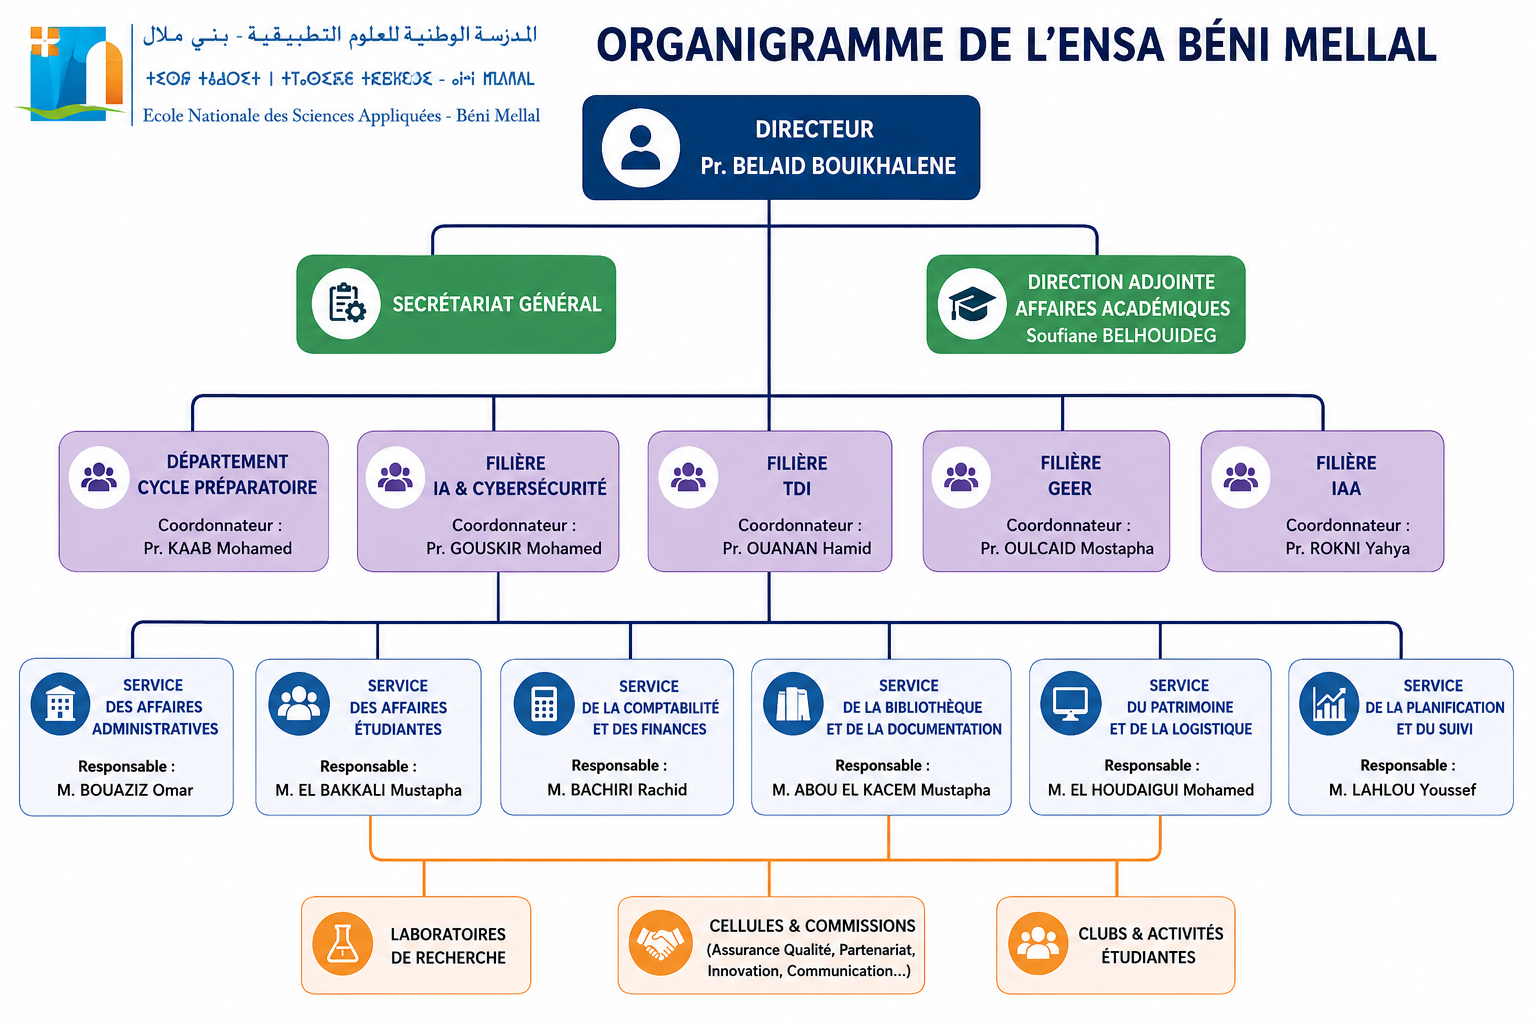
\includegraphics[width=0.95\textwidth]{images/organigrame.png}}
{\fbox{\parbox[c][5cm][c]{0.85\textwidth}{\centering Emplacement réservé pour l’organigramme de l’établissement\\\texttt{images/organigrame.png}}}}
\caption{Organigramme de l’ENSA Béni Mellal}
\label{fig:organigramme-ensa}
\end{figure}

La figure \ref{fig:organigramme-ensa} présente l’organisation générale de l’établissement. Cette structure permet de situer le projet dans son environnement académique et de comprendre le cadre institutionnel dans lequel il a été réalisé.

\section{Contexte du stage}

Le projet a été réalisé dans un contexte académique orienté vers l’innovation numérique et l’Industrie 4.0. Les FabLabs constituent aujourd’hui des espaces importants pour l’apprentissage pratique, le prototypage rapide et la fabrication numérique. Ils mettent à disposition des machines telles que les imprimantes 3D, les machines CNC ou les découpeuses laser.

Cependant, l’accès à ces équipements peut être limité par plusieurs contraintes : disponibilité des machines, besoin de présence physique, difficulté de supervision à distance et absence d’outils unifiés permettant de relier gestion, simulation et analyse de données.

Dans ce contexte, la création d’un FabLab virtuel représente une réponse pertinente. Elle permet de préparer les utilisateurs avant l’utilisation réelle des machines, de simuler des trajectoires de fabrication et d’introduire une couche de supervision intelligente fondée sur les données. Les données utilisées dans cette version sont simulées afin de valider l’architecture, les flux MQTT, le monitoring et le module d’analyse. La plateforme reste conçue pour être connectée ultérieurement à des capteurs réels.

\section{Problématique}

Les FabLabs traditionnels reposent principalement sur une interaction physique avec les équipements. Cette approche est utile pour l’apprentissage pratique, mais elle présente certaines limites dans un contexte pédagogique moderne. Les étudiants ne disposent pas toujours d’un moyen simple pour visualiser les machines, tester un fichier de fabrication ou consulter l’état des équipements avant une séance.

Par ailleurs, les machines de fabrication numérique produisent ou pourraient produire des données de fonctionnement telles que la température, la vibration, la durée d’utilisation, la vitesse du moteur ou les erreurs signalées. Ces données sont précieuses pour la supervision et la maintenance, mais elles restent souvent peu exploitées dans un cadre académique. Dans la version réalisée, ces mesures ne proviennent pas encore de capteurs physiques : elles sont générées par un simulateur MQTT afin de tester les traitements et les interfaces dans des conditions contrôlées.

La problématique du projet peut donc être formulée ainsi :

\begin{center}
\textit{Comment concevoir et réaliser une plateforme virtuelle permettant de gérer un FabLab, de simuler ses machines et d’exploiter des données IoT simulées pour la supervision intelligente et la maintenance prédictive ?}
\end{center}

\section{Objectifs du projet}

L’objectif principal du projet est de concevoir et développer une plateforme web nommée \textbf{Virtual FabLab}, intégrant la gestion des utilisateurs et des machines, la visualisation 3D, la simulation de fichiers de fabrication et l’exploitation de données IoT simulées.

Les objectifs spécifiques sont les suivants :

\begin{itemize}
    \item mettre en place une interface web moderne destinée aux étudiants et aux administrateurs ;
    \item permettre l’inscription, l’authentification et la gestion des profils utilisateurs ;
    \item gérer les machines du FabLab, leurs types, leurs états et leur positionnement dans l’espace 3D ;
    \item offrir un système de réservation des machines avec validation administrative ;
    \item construire une scène 3D interactive représentant le FabLab et ses équipements ;
    \item simuler le comportement d’une imprimante 3D et d’une machine CNC à partir de fichiers G-code ou NC ;
    \item intégrer une télémétrie simulée transmise via MQTT ;
    \item analyser les données simulées afin de détecter les anomalies et d’estimer l’état de santé des machines ;
    \item classifier les intentions administrateur liées à la supervision et à la maintenance ;
    \item proposer un Copilote IA d’aide à la décision réservé à l’administrateur ;
    \item afficher les indicateurs de supervision dans un tableau de bord administrateur.
\end{itemize}

\section{Présentation générale du Virtual FabLab}

La plateforme Virtual FabLab est conçue comme une application web complète reposant sur une architecture frontend/backend. Le frontend assure l’expérience utilisateur, la visualisation du laboratoire virtuel, les interfaces de réservation, les écrans administrateur et les vues de simulation. Le backend fournit les API, la persistance des données, l’authentification, la gestion des rôles, la réception des données MQTT et les services d’analyse.

La solution réalisée couvre plusieurs modules complémentaires :

\begin{itemize}
    \item un module d’authentification basé sur des jetons JWT ;
    \item un module de gestion des utilisateurs et des droits d’accès ;
    \item un module de gestion des machines et de leurs emplacements dans le FabLab virtuel ;
    \item un module de réservation avec suivi des demandes ;
    \item un module de visualisation 3D du laboratoire ;
    \item un module de simulation G-code pour imprimante 3D et CNC ;
    \item un module MQTT permettant l’ingestion de télémétrie simulée ;
    \item un module Data Science et IA pour la détection d’anomalies, le score de santé, l’estimation indicative du risque de maintenance, la classification d’intentions et le Copilote IA d’aide à la décision.
\end{itemize}

\begin{figure}[H]
\centering
\IfFileExists{images/vue_generale_virtual_fablab.png}
{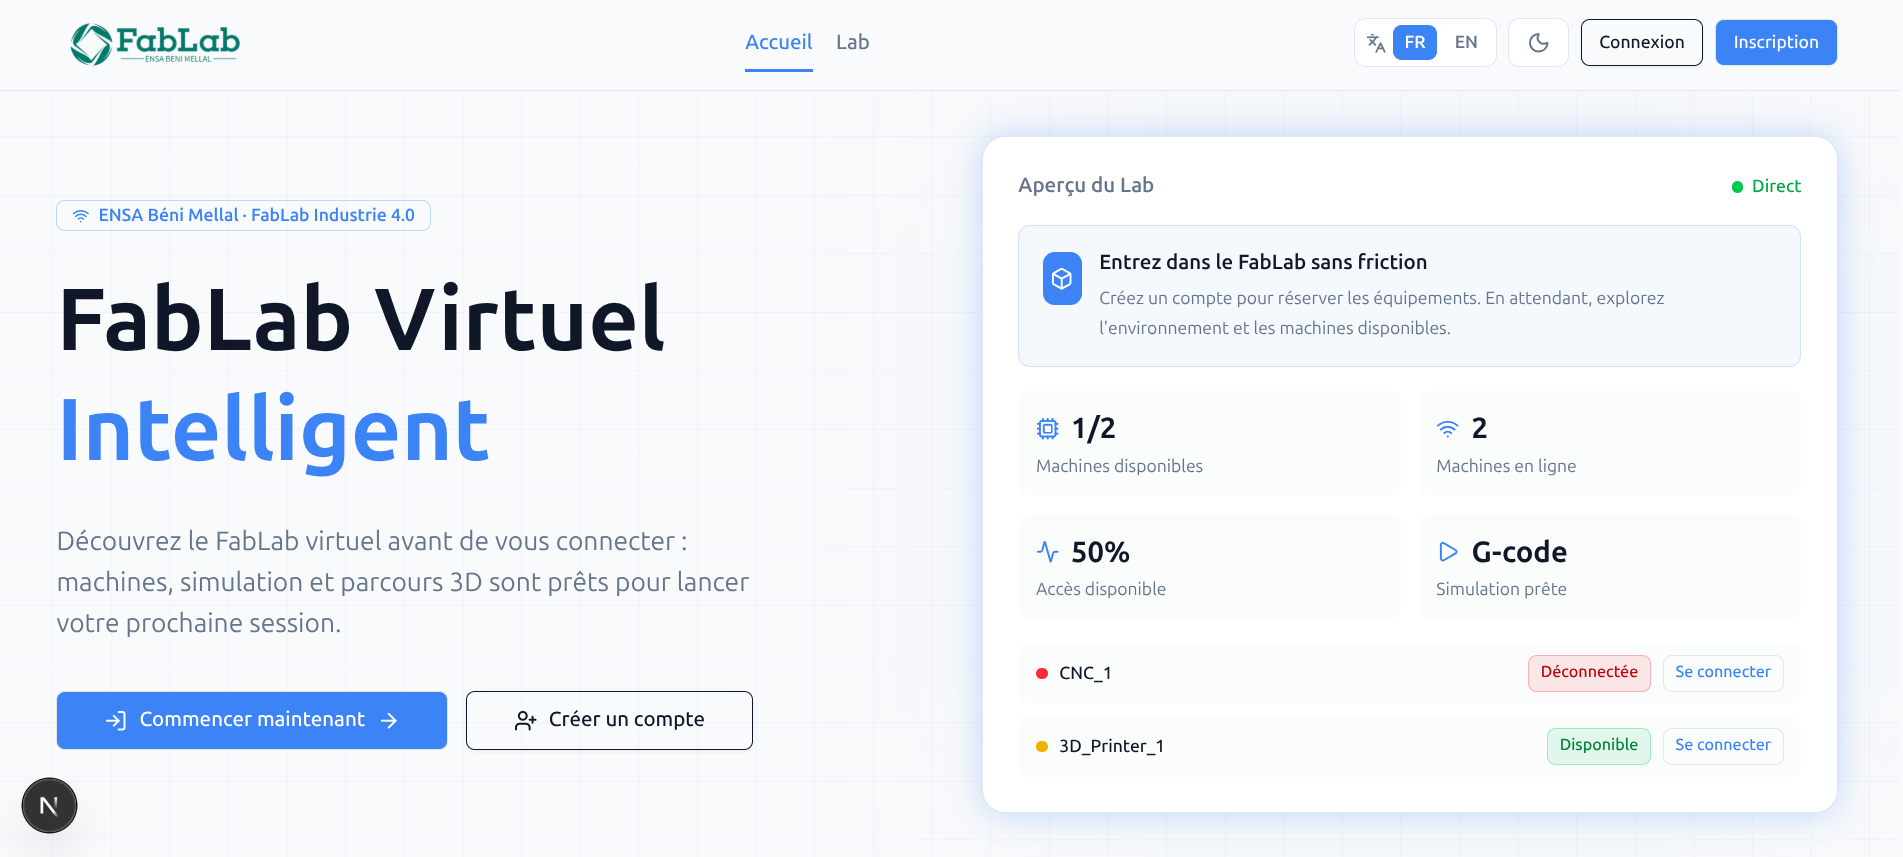
\includegraphics[width=0.9\textwidth]{images/vue_generale_virtual_fablab.png}}
{\fbox{\parbox[c][5cm][c]{0.85\textwidth}{\centering Emplacement réservé pour une vue générale de la plateforme\\\texttt{images/vue\_generale\_virtual\_fablab.png}}}}
\caption{Vue générale prévue de la plateforme Virtual FabLab}
\label{fig:vue-generale-virtual-fablab}
\end{figure}

\section{Conclusion}

Ce chapitre a présenté l’organisme d’accueil, le contexte général du projet, la problématique ainsi que les objectifs de la plateforme Virtual FabLab. Le projet se positionne à l’intersection du développement web, de la simulation 3D, de l’IoT et de la Data Science.

Le chapitre suivant sera consacré à l’analyse des besoins et à la conception du système. Il présentera les acteurs, les fonctionnalités attendues, l’architecture générale, les modules de la plateforme ainsi que les technologies retenues pour la réalisation.

\chapter{Analyse des besoins et conception}

\section{Introduction}

Après avoir présenté le cadre général du projet, ce chapitre détaille l’analyse des besoins et la conception de la plateforme Virtual FabLab. L’objectif est de formaliser les fonctionnalités attendues, les contraintes de qualité, les acteurs du système, puis de proposer une architecture technique cohérente avec l’implémentation réalisée.

La conception retenue s’appuie sur une application web composée d’un frontend interactif, d’un backend applicatif, d’une base de données, d’un flux MQTT simulé et d’un module d’analyse de données.

\section{Étude des besoins}

L’étude des besoins vise à identifier les services que la plateforme doit fournir aux utilisateurs. Le système doit répondre à deux catégories principales d’utilisateurs : les étudiants et les administrateurs.

L’étudiant doit pouvoir accéder au FabLab virtuel, consulter les machines disponibles, réserver un créneau et tester un fichier de fabrication dans une simulation 3D. L’administrateur doit disposer d’un espace de pilotage lui permettant de gérer les machines, les utilisateurs, les réservations et les indicateurs de supervision.

Le système doit également être capable de recevoir des données simulées issues des machines, de les stocker et de les exploiter pour la détection d’anomalies et l’aide à la maintenance. Les données utilisées dans cette version sont simulées afin de valider l’architecture, les flux MQTT, le monitoring et le module d’analyse. La plateforme reste conçue pour être connectée ultérieurement à des capteurs réels.

\section{Besoins fonctionnels}

\subsection{Besoins de l’étudiant}

Les fonctionnalités attendues pour l’étudiant sont les suivantes :

\begin{itemize}
    \item créer un compte utilisateur ;
    \item s’authentifier et accéder à un espace personnel ;
    \item consulter les machines disponibles dans le FabLab ;
    \item visualiser le laboratoire virtuel en 3D ;
    \item sélectionner une machine et consulter ses informations ;
    \item effectuer une demande de réservation sur un créneau disponible ;
    \item consulter l’historique de ses réservations ;
    \item importer un fichier G-code ou NC compatible ;
    \item lancer, mettre en pause et réinitialiser une simulation ;
    \item modifier les informations de son profil.
\end{itemize}

\subsection{Besoins de l’administrateur}

Les fonctionnalités attendues pour l’administrateur sont les suivantes :

\begin{itemize}
    \item consulter un tableau de bord global ;
    \item gérer les utilisateurs et leurs rôles ;
    \item activer ou désactiver un compte utilisateur ;
    \item créer, modifier ou supprimer des machines ;
    \item modifier l’état et le placement 3D des machines ;
    \item consulter les demandes de réservation ;
    \item approuver, refuser ou supprimer une réservation ;
    \item superviser les données de télémétrie reçues ;
    \item suivre l’état MQTT du système ;
    \item consulter les alertes d’anomalies ;
    \item consulter les scores de santé et les recommandations de maintenance ;
    \item interroger un Copilote IA de maintenance pour obtenir une synthèse structurée fondée sur les données disponibles.
\end{itemize}

\section{Besoins non fonctionnels}

Les besoins non fonctionnels définissent les qualités attendues de la solution :

\begin{itemize}
    \item \textbf{Sécurité} : les fonctionnalités sensibles doivent être protégées par authentification et contrôle de rôle.
    \item \textbf{Ergonomie} : l’interface doit être claire, lisible et adaptée à un usage pédagogique.
    \item \textbf{Maintenabilité} : le code doit être organisé en modules séparant les responsabilités.
    \item \textbf{Évolutivité} : la solution doit permettre l’ajout de nouveaux types de machines ou de nouveaux indicateurs.
    \item \textbf{Performance} : la scène 3D et la simulation doivent rester fluides dans un navigateur moderne.
    \item \textbf{Traçabilité} : les données de télémétrie doivent être conservées afin d’alimenter l’historique et les analyses.
    \item \textbf{Interopérabilité} : les échanges entre frontend et backend doivent être réalisés à travers des API structurées.
\end{itemize}

\section{Acteurs du système}

Le système met en interaction plusieurs acteurs :

\begin{itemize}
    \item \textbf{Étudiant} : utilisateur inscrit qui consulte les machines, réserve des créneaux et lance des simulations.
    \item \textbf{Administrateur} : utilisateur disposant de droits avancés pour gérer la plateforme et superviser les machines.
    \item \textbf{Broker MQTT} : composant intermédiaire chargé de transmettre les messages de télémétrie simulée.
    \item \textbf{Machine simulée} : source logique des données de fonctionnement publiées dans le système.
\end{itemize}

\section{Cas d’utilisation}

Le diagramme de cas d’utilisation permet de représenter les interactions principales entre les acteurs et la plateforme.

\begin{figure}[H]
\centering
\IfFileExists{images/diagrame_user.png}
{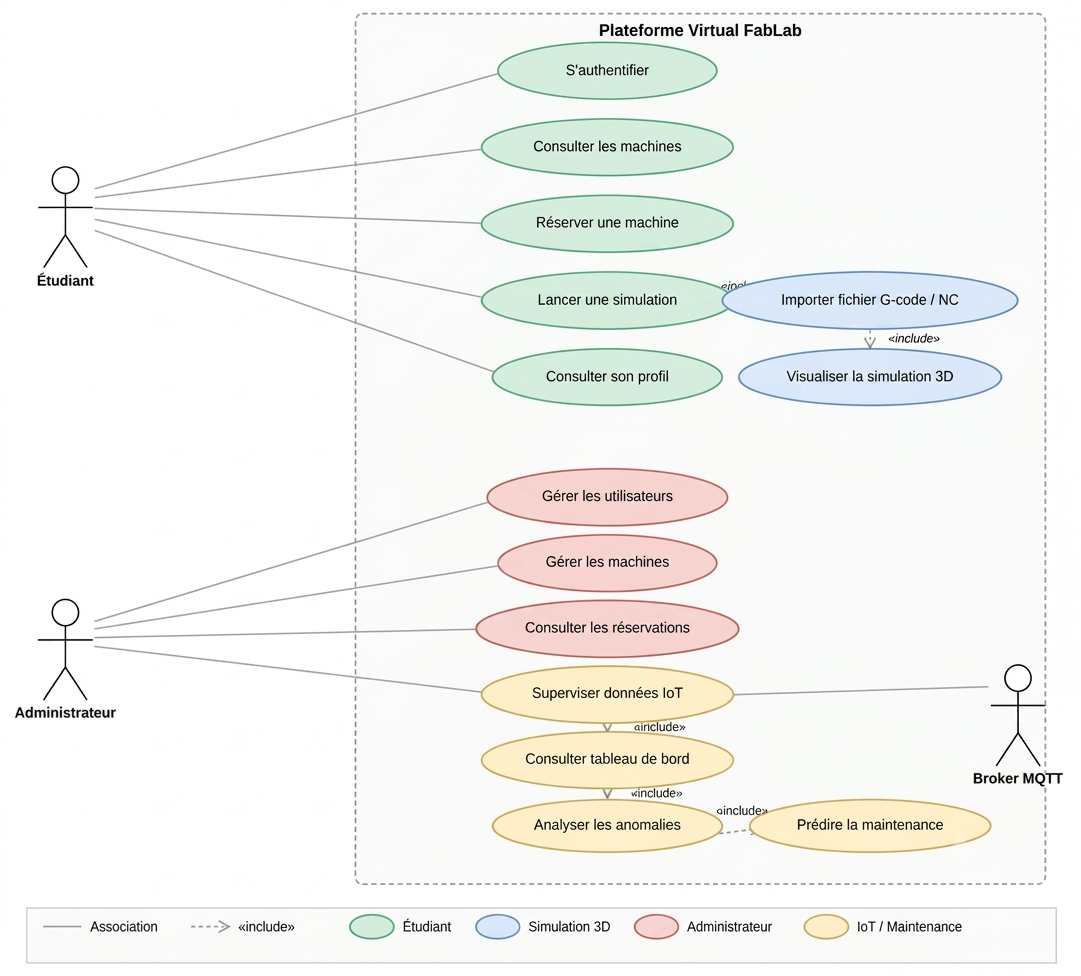
\includegraphics[width=0.95\textwidth]{images/diagrame_user.png}}
{\fbox{\parbox[c][5cm][c]{0.85\textwidth}{\centering Emplacement réservé pour le diagramme de cas d’utilisation\\\texttt{images/diagrame\_user.png}}}}
\caption{Diagramme de cas d’utilisation de la plateforme Virtual FabLab}
\label{fig:diagramme-cas-utilisation}
\end{figure}

Les cas d’utilisation principaux sont l’authentification, la consultation des machines, la réservation, la simulation, la gestion administrative, la supervision IoT et l’analyse des anomalies.

\section{Architecture générale}

L’architecture générale de la plateforme repose sur une séparation claire entre l’interface utilisateur, les services backend, la base de données, le flux MQTT et le module Data Science.

\begin{figure}[H]
\centering
\IfFileExists{images/architecture_generale.png}
{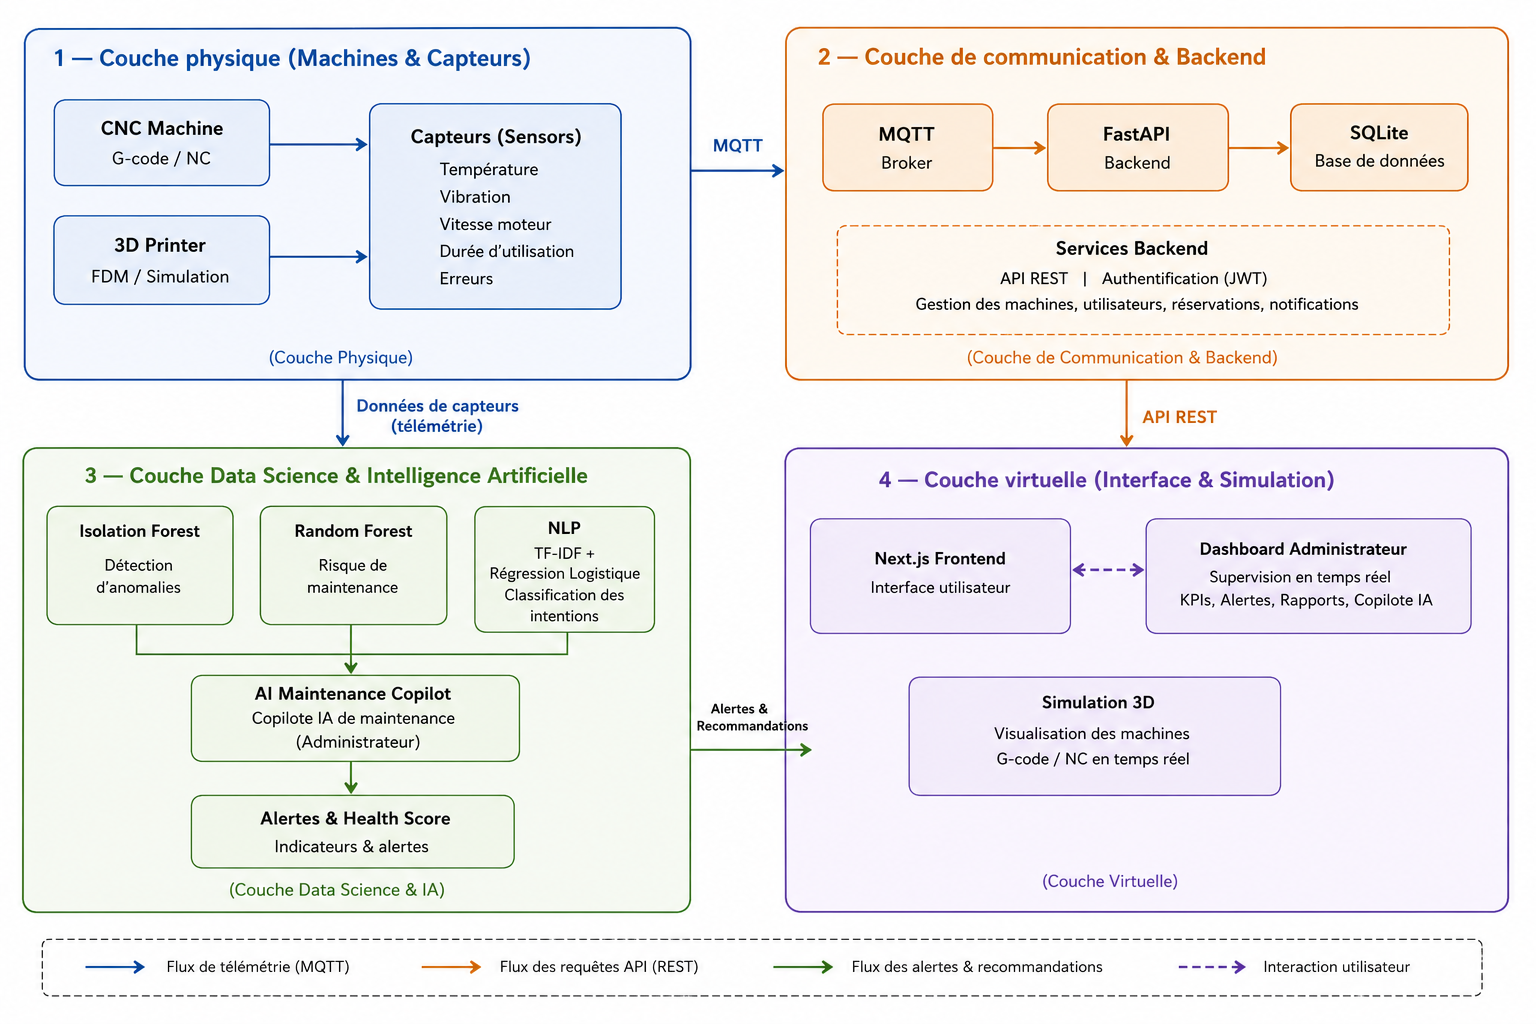
\includegraphics[width=0.95\textwidth]{images/architecture_generale.png}}
{\fbox{\parbox[c][5.5cm][c]{0.85\textwidth}{\centering Emplacement réservé pour le schéma d’architecture générale\\\texttt{images/architecture\_generale.png}}}}
\caption{Architecture générale de la plateforme Virtual FabLab}
\label{fig:architecture-generale}
\end{figure}

Le frontend communique avec le backend à travers des requêtes HTTP. Le backend expose les API, gère la base de données SQLite et lance un abonné MQTT au démarrage de l’application. Les messages reçus sont transformés en mesures de télémétrie puis exploités par les services de monitoring et de prédiction.

\section{Description des modules}

La plateforme est structurée autour des modules suivants :

\begin{itemize}
    \item \textbf{Module d’authentification} : inscription, connexion, profil, changement de mot de passe et génération de jetons JWT.
    \item \textbf{Module utilisateurs} : liste, recherche, changement de rôle et activation ou désactivation des comptes.
    \item \textbf{Module machines} : gestion des types de machines, des instances, de leurs états et de leurs coordonnées dans le laboratoire 3D.
    \item \textbf{Module réservations} : création des demandes, calcul des créneaux disponibles, annulation et validation par l’administrateur.
    \item \textbf{Module FabLab 3D} : visualisation interactive de la salle et des machines avec sélection et consultation de leur état.
    \item \textbf{Module simulation} : importation et interprétation des fichiers G-code ou NC pour l’imprimante 3D et la CNC.
    \item \textbf{Module MQTT} : réception des données simulées publiées sur les topics machines.
    \item \textbf{Module Data Science et IA} : détection d’anomalies avec Isolation Forest, estimation du risque de maintenance avec Random Forest Classifier, calcul du score de santé, classification supervisée des intentions administrateur et Copilote IA d’aide à la décision.
    \item \textbf{Module notifications} : notification des étudiants après validation ou refus d’une réservation.
\end{itemize}

\section{Diagramme de classes}

Le diagramme de classes représente les entités principales utilisées dans la base de données et leurs relations : utilisateur, machine, type de machine, réservation, mesure capteur et notification.

\begin{figure}[H]
\centering
\IfFileExists{images/class.png}
{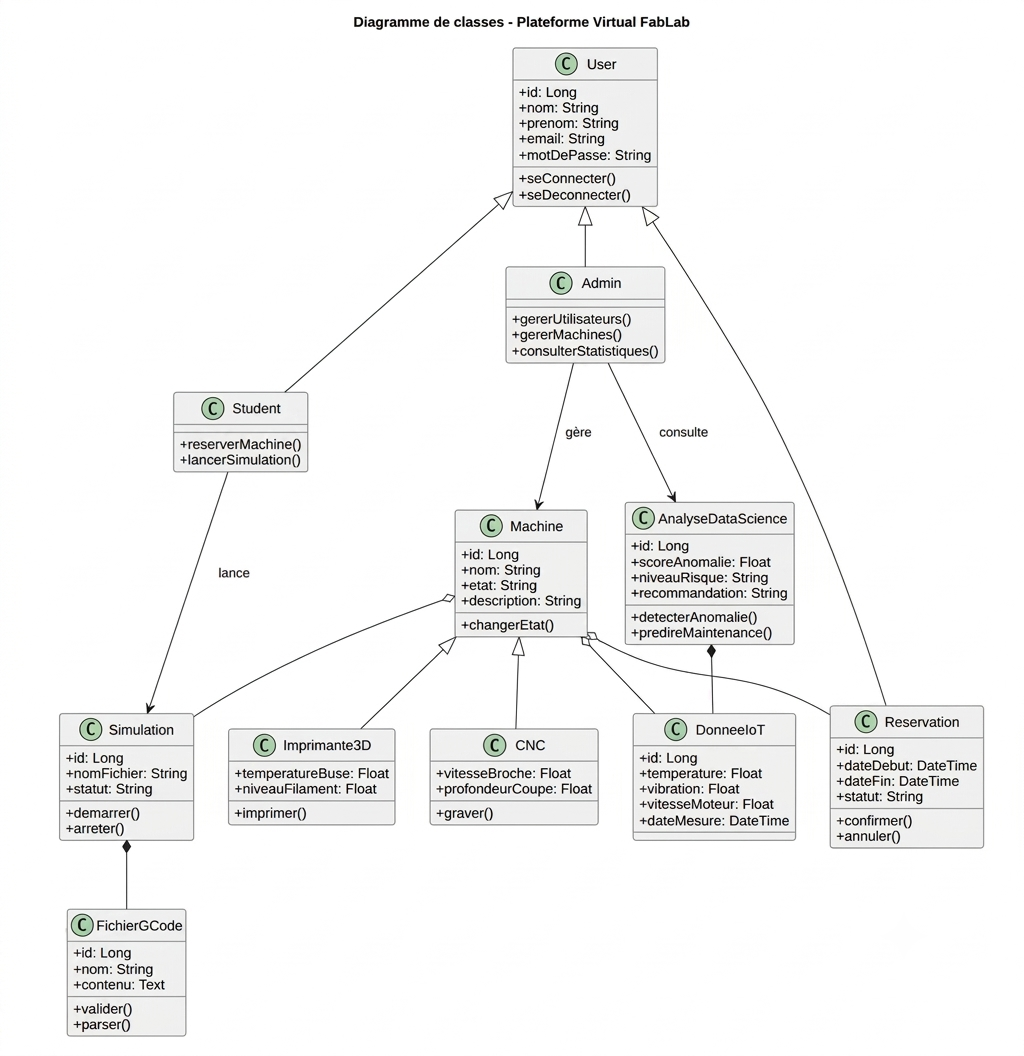
\includegraphics[width=0.95\textwidth]{images/class.png}}
{\fbox{\parbox[c][5cm][c]{0.85\textwidth}{\centering Emplacement réservé pour le diagramme de classes\\\texttt{images/class.png}}}}
\caption{Diagramme de classes de la plateforme Virtual FabLab}
\label{fig:diagramme-classes}
\end{figure}

La conception des données distingue les types de machines des instances de machines. Cette séparation permet d’associer un modèle 3D, un schéma de capteurs et des informations techniques à un type, tout en laissant chaque instance posséder son propre nom, état et emplacement.

\section{Conception du système}

\subsection{Conception de l’authentification}

Le système d’authentification repose sur des jetons JWT. Après connexion, le backend renvoie un jeton d’accès utilisé par le frontend pour appeler les routes protégées. Le rôle de l’utilisateur permet de distinguer les droits d’un étudiant et ceux d’un administrateur.

\subsection{Conception de la gestion des machines}

Chaque machine possède un type, un nom unique, un état, des notes et des paramètres de placement dans la scène 3D. Les machines peuvent être consultées par les utilisateurs, tandis que leur création, modification ou suppression est réservée à l’administrateur.

\subsection{Conception de la réservation}

Le système de réservation repose sur des créneaux d’une heure entre 8h00 et 20h00. Une demande est créée avec l’état \texttt{pending}. L’administrateur peut ensuite l’approuver ou la refuser. Les conflits sont évités en vérifiant les réservations actives pour la même machine et le même intervalle.

\subsection{Conception de la télémétrie}

Dans l’implémentation actuelle, la télémétrie simulée est reçue sous forme de messages JSON publiés via MQTT. Le backend associe chaque message à une machine existante, enregistre les mesures et expose l’historique à travers les routes de monitoring.

\subsection{Conception de l’analyse intelligente}

Le module Data Science et IA combine des modèles entraînés avec scikit-learn et une logique par règles. La détection d’anomalies s’appuie sur un modèle \textit{Isolation Forest}, tandis que l’estimation du risque de maintenance repose sur un \textit{Random Forest Classifier}. Une logique complémentaire par règles est utilisée pour consolider le score de santé, le niveau de risque et les recommandations de maintenance, notamment lorsque les modèles ne sont pas disponibles ou lorsqu’une lecture doit être interprétée de manière explicable.

Les variables analysées sont la température, la vibration, la durée d’utilisation exprimée sous forme \texttt{usage\_duration} puis convertie en \texttt{usage\_hours}, la vitesse du moteur \texttt{motor\_speed} et l’historique des erreurs signalées. Les sorties produites par le module sont le statut d’anomalie, la probabilité indicative de risque, le score de santé, le niveau de risque et une recommandation de maintenance.

Le même module intègre également une classification supervisée des intentions administrateur, fondée sur TF-IDF et Logistic Regression, afin d’alimenter un Copilote IA de maintenance. Ce copilote ne correspond pas à un LLM ni à une IA générative ; il fournit des réponses déterministes construites à partir des données de la plateforme, des résultats analytiques et de l’intention reconnue.

\section{Technologies utilisées}

\newcommand{\techitem}[3]{%
  \subsection{#1}
  \noindent
  \begin{minipage}[c]{0.22\textwidth}
    \centering
    \IfFileExists{#2}
    {\includegraphics[width=0.85\linewidth,height=1.8cm,keepaspectratio]{#2}}
    {\fbox{\parbox[c][1.8cm][c]{0.85\linewidth}{\centering\scriptsize #1}}}
  \end{minipage}
  \hfill
  \begin{minipage}[c]{0.72\textwidth}
    #3
  \end{minipage}
  \par\vspace{0.4cm}
}

\techitem{Next.js}{images/nextjs.png}{Next.js est un framework basé sur React permettant de développer des applications web modernes, modulaires et performantes. Dans ce projet, il constitue la base du frontend. Il organise les pages de l’application, les composants d’interface, les appels API et les vues interactives destinées aux étudiants et aux administrateurs.}

\techitem{FastAPI}{images/fastapi.jpg}{FastAPI est un framework Python destiné à la création d’API web rapides et structurées. Il est utilisé pour implémenter le backend de la plateforme : authentification, gestion des machines, réservations, monitoring, réception MQTT et services d’analyse.}

\techitem{Three.js}{images/threejs.png}{Three.js est une bibliothèque JavaScript permettant de créer des scènes 3D dans le navigateur. Elle est utilisée pour afficher le laboratoire virtuel, charger les modèles GLB des machines et animer les trajectoires issues des fichiers de fabrication.}

\techitem{Blender}{images/blender.png}{Blender est un logiciel de modélisation 3D open source. Il intervient dans la préparation et l’optimisation des modèles 3D utilisés dans la plateforme, notamment ceux de l’imprimante 3D et de la machine CNC.}

\techitem{MQTT}{images/mqtt.png}{MQTT est un protocole léger de communication publish/subscribe très utilisé dans les systèmes IoT. Dans ce projet, il permet de simuler l’envoi de mesures machines vers le backend à l’aide d’un simulateur MQTT. Les messages sont publiés sur des topics propres à chaque machine, selon le motif suivant :

\begin{center}
\small\texttt{fablab/machines/\{machine\_id\}/data}
\end{center}}

\techitem{Python}{images/python.png}{Python est utilisé côté backend pour développer les services applicatifs et les traitements de données. Il facilite également l’intégration des bibliothèques de Data Science et l’entraînement des modèles.}

\techitem{Tailwind CSS}{images/tailwind.png}{Tailwind CSS est un framework CSS utilitaire permettant de construire rapidement des interfaces cohérentes et responsives. Dans la plateforme, il est utilisé pour structurer les pages, les cartes, les tableaux, les formulaires et les tableaux de bord.}

\techitem{Scikit-learn}{images/scikit_learn.png}{Scikit-learn est une bibliothèque Python dédiée au Machine Learning. Elle est utilisée dans ce projet pour entraîner et exploiter un modèle de détection d’anomalies de type Isolation Forest et un Random Forest Classifier pour l’estimation du risque de maintenance.}

\techitem{Visual Studio Code}{images/vscode.png}{Visual Studio Code est l’environnement de développement utilisé pour organiser et modifier les différents modules du projet : frontend, backend, simulation, scripts Python et fichiers LaTeX du rapport.}

\newcommand{\iotitem}[3]{%
  \subsubsection{#1}
  \noindent
  \begin{minipage}[c]{0.22\textwidth}
    \centering
    \IfFileExists{#2}
    {\includegraphics[width=0.85\linewidth,height=1.8cm,keepaspectratio]{#2}}
    {\fbox{\parbox[c][1.8cm][c]{0.85\linewidth}{\centering\scriptsize #1}}}
  \end{minipage}
  \hfill
  \begin{minipage}[c]{0.72\textwidth}
    #3
  \end{minipage}
  \par\vspace{0.4cm}
}

\subsection{Technologies et équipements IoT}

Cette partie présente les composants matériels et les équipements de fabrication numérique liés à la dimension IoT du FabLab. Dans la version actuelle, ils servent de référence pour concevoir les mesures et les scénarios de supervision. La collecte effective n’est pas encore réalisée par des capteurs physiques : elle est simulée par MQTT afin de valider les flux, le stockage et l’analyse avant une intégration matérielle future.

\iotitem{ESP8266}{images/esp8266.jpg}{L’ESP8266 est un microcontrôleur doté d’une connectivité Wi-Fi intégrée, largement utilisé dans les applications de l’Internet des Objets. Dans un contexte FabLab, il peut servir d’interface entre les capteurs physiques et la plateforme de supervision. Il permet de collecter des mesures, de les traiter localement puis de les transmettre vers un serveur ou un broker MQTT. Son faible coût et sa facilité de programmation en font un choix adapté aux prototypes académiques et industriels légers.}

\iotitem{Capteur de température}{images/DHT.jpg}{Le capteur de température permet de mesurer l’échauffement d’un environnement, d’un composant électronique ou d’une machine en fonctionnement. Dans le cadre d’un FabLab intelligent, cette donnée est utile pour surveiller les conditions de travail et prévenir les situations anormales. Une température excessive peut indiquer une surcharge, un défaut de ventilation ou une dégradation progressive d’un équipement. Lors d’une connexion future à des capteurs réels, ces mesures pourront alimenter des tableaux de bord et des modèles de maintenance prédictive.}

\iotitem{Capteur de vibration}{images/capteur_vibration.jpg}{Le capteur de vibration mesure les oscillations mécaniques produites par une machine pendant son fonctionnement. Ces données sont essentielles pour les équipements de fabrication numérique, car des vibrations inhabituelles peuvent révéler un désalignement, une usure ou un défaut mécanique. Dans une approche de maintenance préventive, l’analyse de ces signaux aide à identifier les anomalies avant l’apparition d’une panne. Les données de vibration constituent ainsi un indicateur pertinent de l’état de santé des machines.}

\iotitem{Imprimante 3D}{images/imprimante_3d.png}{L’imprimante 3D est un équipement de fabrication additive permettant de produire des objets physiques à partir de modèles numériques. Elle fonctionne généralement par dépôt progressif de matière selon des trajectoires définies dans un fichier G-code. Dans un FabLab, elle constitue un outil pédagogique et technique essentiel pour le prototypage rapide. Son intégration à une plateforme IoT permet de suivre son état, sa température, sa progression et ses éventuelles anomalies de fonctionnement.}

\iotitem{Machine CNC}{images/cnc.jpg}{La machine CNC est un équipement de fabrication soustractive commandé numériquement. Elle exécute des opérations d’usinage à partir d’instructions précises, souvent décrites dans des fichiers NC ou G-code. Dans un FabLab, elle permet de travailler différents matériaux avec une grande précision. La supervision IoT d’une CNC peut porter sur son état, ses vibrations, sa durée d’utilisation et ses paramètres de fonctionnement afin d’améliorer la sécurité, la traçabilité et la maintenance.}

\section{Conclusion}

Ce chapitre a présenté l’analyse des besoins, les acteurs, les cas d’utilisation et la conception générale de la plateforme. Il a également décrit les technologies retenues et leur rôle dans le projet.

Le chapitre suivant sera consacré à la réalisation et à l’implémentation. Il détaillera l’organisation concrète du frontend et du backend, les modules développés, la simulation 3D, le flux MQTT et les interfaces de supervision.

\chapter{Réalisation et implémentation}

\section{Introduction}

Ce chapitre présente la réalisation technique de la plateforme Virtual FabLab. Contrairement au chapitre précédent, qui décrit l’analyse et la conception, cette partie se concentre sur l’implémentation effective du projet : organisation du code, architecture frontend/backend, modules fonctionnels, simulation 3D, communication MQTT et tableau de bord de supervision.

La plateforme réalisée repose sur un backend FastAPI, une interface Next.js et des modules spécialisés pour la visualisation 3D, l’interprétation des fichiers de fabrication et l’analyse des données de télémétrie. Les données utilisées dans cette version sont simulées afin de valider l’architecture, les flux MQTT, le monitoring et le module d’analyse. La plateforme reste conçue pour être connectée ultérieurement à des capteurs réels.

\section{Architecture frontend/backend}

L’implémentation adopte une architecture séparant clairement le frontend et le backend. Le frontend prend en charge l’interface utilisateur, la navigation, les scènes 3D et les tableaux de bord. Le backend fournit les API, la sécurité, la base de données, l’ingestion MQTT et les traitements analytiques.

\begin{figure}[H]
\centering
\IfFileExists{images/implementation_architecture.png}
{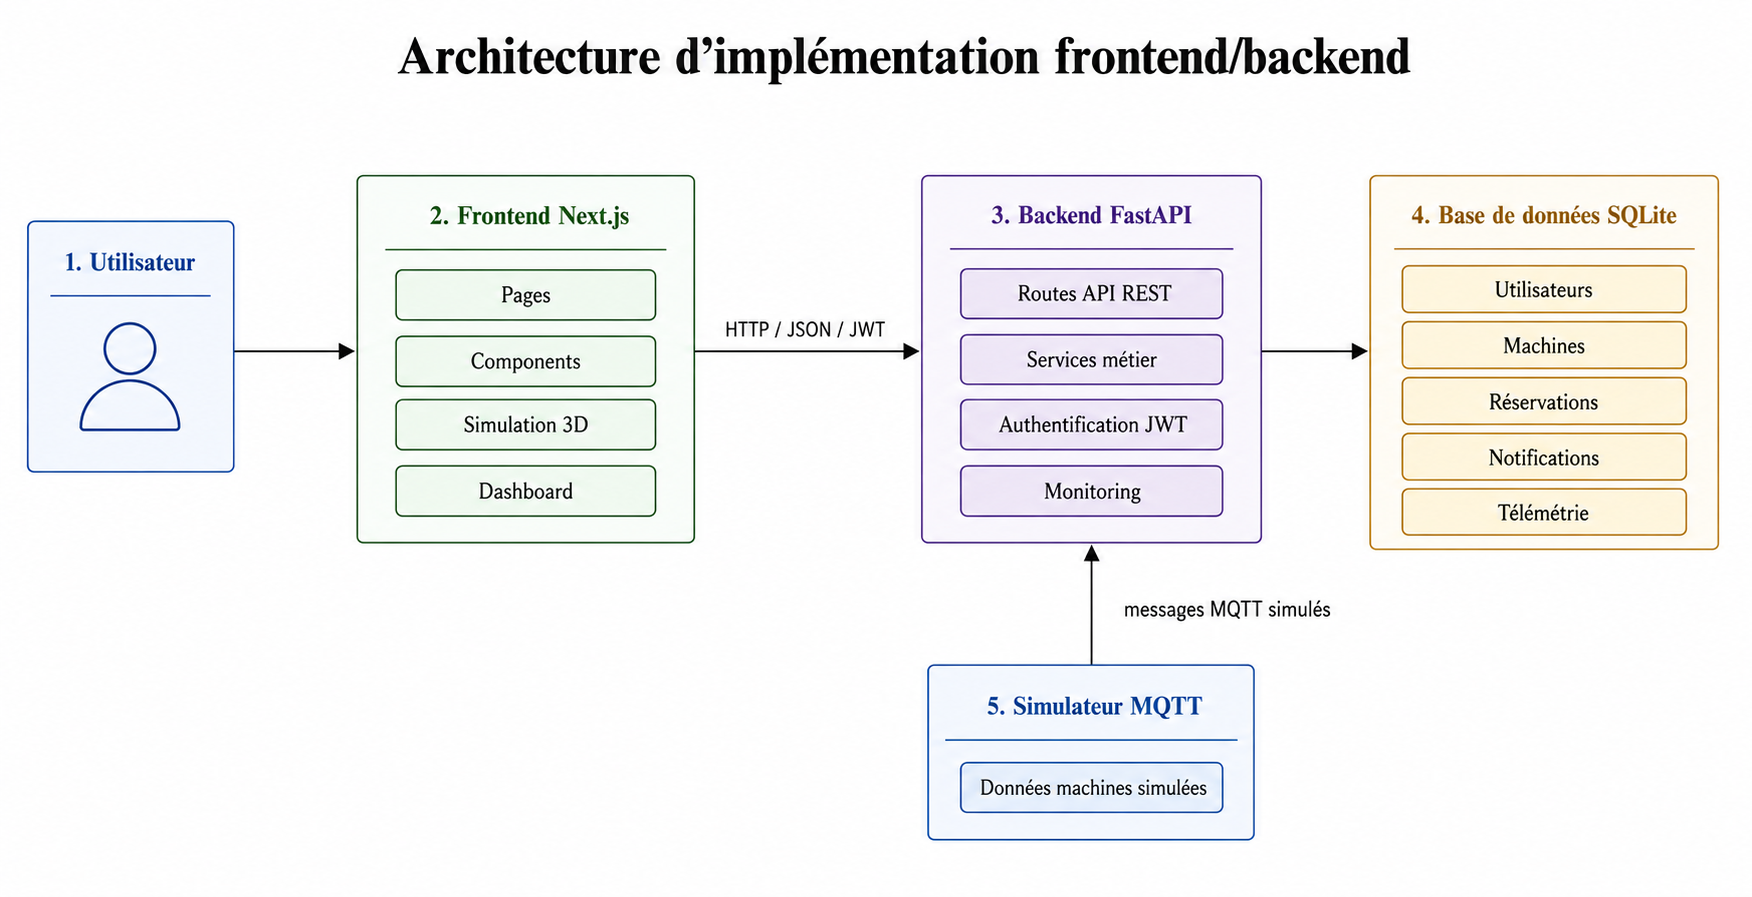
\includegraphics[width=0.95\textwidth]{images/implementation_architecture.png}}
{\fbox{\parbox[c][5.5cm][c]{0.85\textwidth}{\centering Emplacement réservé pour l’architecture d’implémentation\\\texttt{images/implementation\_architecture.png}}}}
\caption{Architecture d’implémentation frontend/backend}
\label{fig:implementation-architecture}
\end{figure}

Le backend est initialisé dans le point d’entrée FastAPI. Au démarrage, il initialise la base de données et lance le service abonné MQTT. Les routes sont ensuite organisées par domaine fonctionnel : authentification, machines, réservations, administration, monitoring, simulation, notifications et intelligence artificielle.

\section{Organisation des dossiers}

Le projet est organisé en trois parties principales : le frontend, le backend et le rapport LaTeX. Cette organisation facilite la maintenance et permet d’isoler les responsabilités.

\begin{table}[H]
\centering
\small
\caption{Organisation générale du projet}
\label{tab:organisation-projet}
\begin{tabular}{|p{0.28\textwidth}|p{0.62\textwidth}|}
\hline
\rowcolor{SectionColor!12}
\textbf{Dossier} & \textbf{Rôle} \\
\hline
\texttt{Frontend/app} & Pages principales de l’application Next.js : accueil, lab 3D, simulation, dashboard, réservations, utilisateurs et profil. \\
\hline
\texttt{Frontend/components} & Composants réutilisables : layout, authentification, scène 3D, simulation, tableaux de bord et composants UI. \\
\hline
\texttt{Frontend/lib} & Fonctions utilitaires, appels API, traductions et moteur d’interprétation des fichiers G-code/NC. \\
\hline
\texttt{backend/app/routes} & Définition des endpoints FastAPI par domaine fonctionnel. \\
\hline
\texttt{backend/app/services} & Logique métier : authentification, machines, réservations, télémétrie, MQTT, anomalies et prédiction. \\
\hline
\texttt{backend/app/models} & Modèles SQLModel représentant les entités persistées. \\
\hline
\texttt{backend/scripts} & Scripts de simulation MQTT et d’entraînement des modèles de Machine Learning. \\
\hline
\texttt{Rapport\_PFE} & Sources LaTeX du rapport académique. \\
\hline
\end{tabular}
\end{table}

\section{Implémentation du backend}

\subsection{API FastAPI}

Le backend expose une API REST structurée autour de plusieurs routeurs. Chaque routeur regroupe les endpoints liés à un domaine précis. Cette organisation améliore la lisibilité du code et facilite l’évolution de la plateforme.

Les principales familles d’endpoints sont :

\begin{itemize}
    \item \texttt{/auth} pour l’inscription, la connexion et le profil ;
    \item \texttt{/machines} pour la gestion administrative des machines ;
    \item \texttt{/lab/machines} pour l’affichage public des machines du FabLab ;
    \item \texttt{/reservations} pour les demandes de réservation ;
    \item \texttt{/admin} pour la gestion des utilisateurs et des réservations ;
    \item \texttt{/monitoring} pour la télémétrie et l’état MQTT ;
    \item \texttt{/simulation} pour l’état de simulation ;
    \item \texttt{/admin/ai} pour les analyses intelligentes réservées à l’administrateur.
\end{itemize}

\subsection{Base de données}

La persistance est assurée par SQLite avec SQLModel. Les modèles principaux sont les utilisateurs, les types de machines, les machines, les réservations, les mesures capteurs et les notifications.

\begin{figure}[H]
\centering
\IfFileExists{images/database_schema.png}
{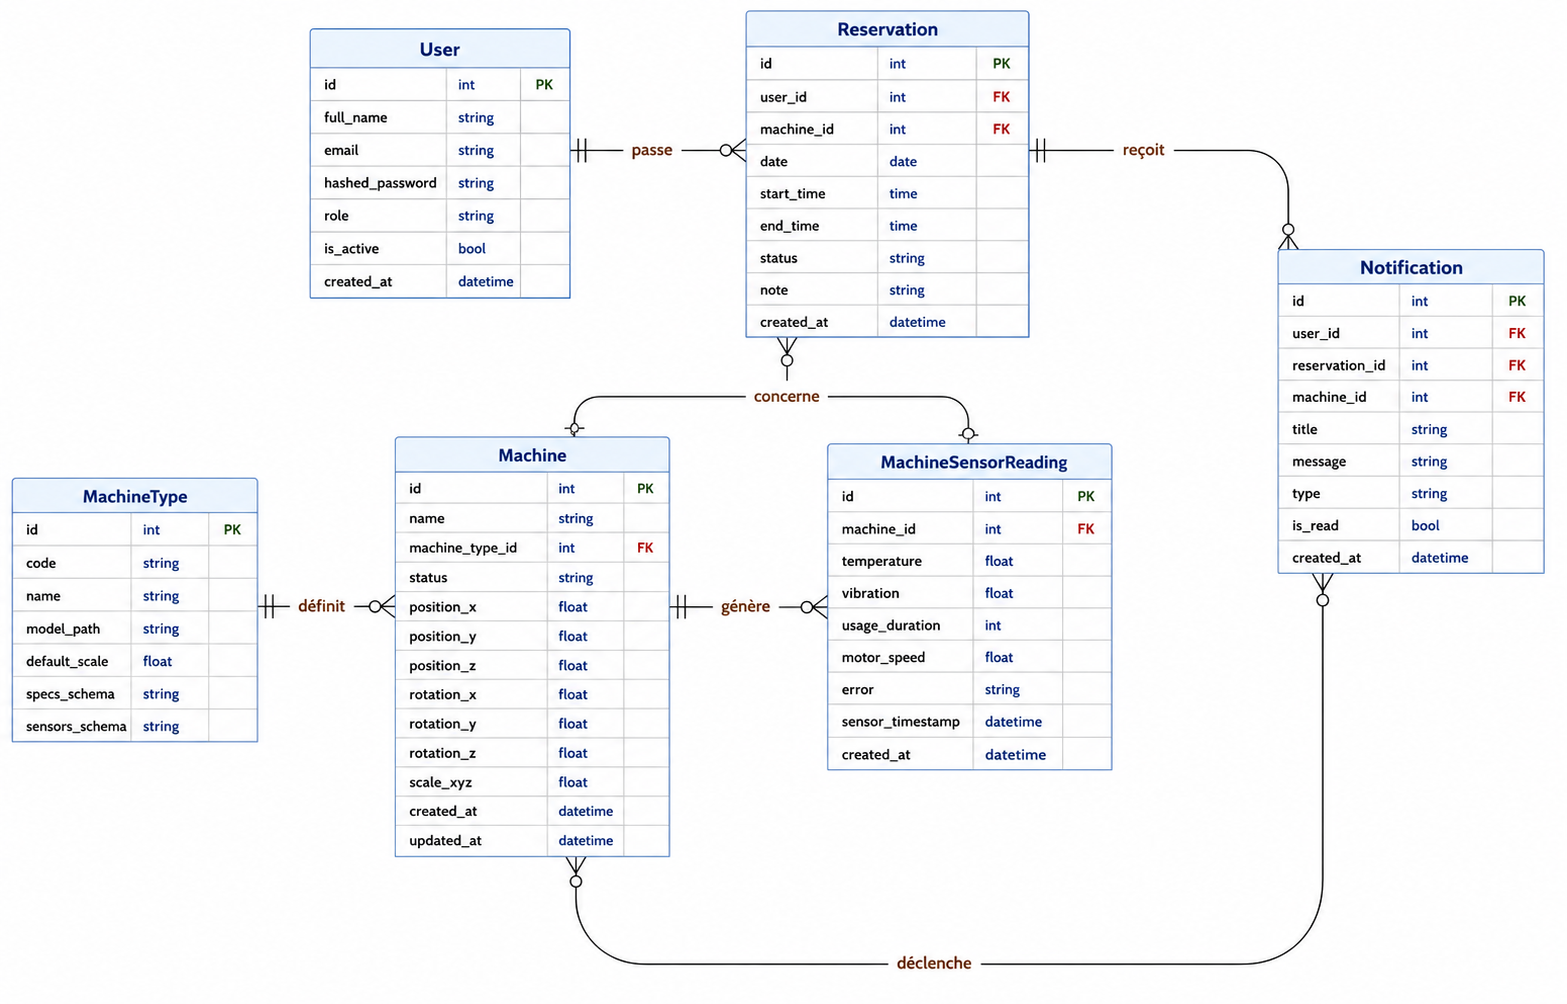
\includegraphics[width=0.95\textwidth,height=0.65\textheight,keepaspectratio]{images/database_schema.png}}
{\fbox{\parbox[c][5cm][c]{0.85\textwidth}{\centering Emplacement réservé pour le schéma de la base de données\\\texttt{images/database\_schema.png}}}}
\caption{Schéma logique de la base de données}
\label{fig:database-schema}
\end{figure}

\section{Système d’authentification}

L’authentification est basée sur des jetons JWT. Lorsqu’un utilisateur se connecte, le backend vérifie son email et son mot de passe haché, puis génère un jeton d’accès. Le frontend conserve ce jeton et l’ajoute dans l’en-tête \texttt{Authorization} lors des appels aux routes protégées.

Deux rôles sont définis dans le système :

\begin{itemize}
    \item \texttt{student} : rôle par défaut pour les utilisateurs inscrits ;
    \item \texttt{admin} : rôle permettant l’accès aux interfaces et endpoints d’administration.
\end{itemize}

\section{Gestion des utilisateurs et de l’administration}

L’espace administrateur permet de consulter les utilisateurs, de rechercher un compte, de filtrer par rôle ou par état, puis de modifier les droits. L’administrateur peut également activer ou désactiver un compte.

\begin{figure}[H]
\centering
\IfFileExists{images/screenshot_users_admin.png}
{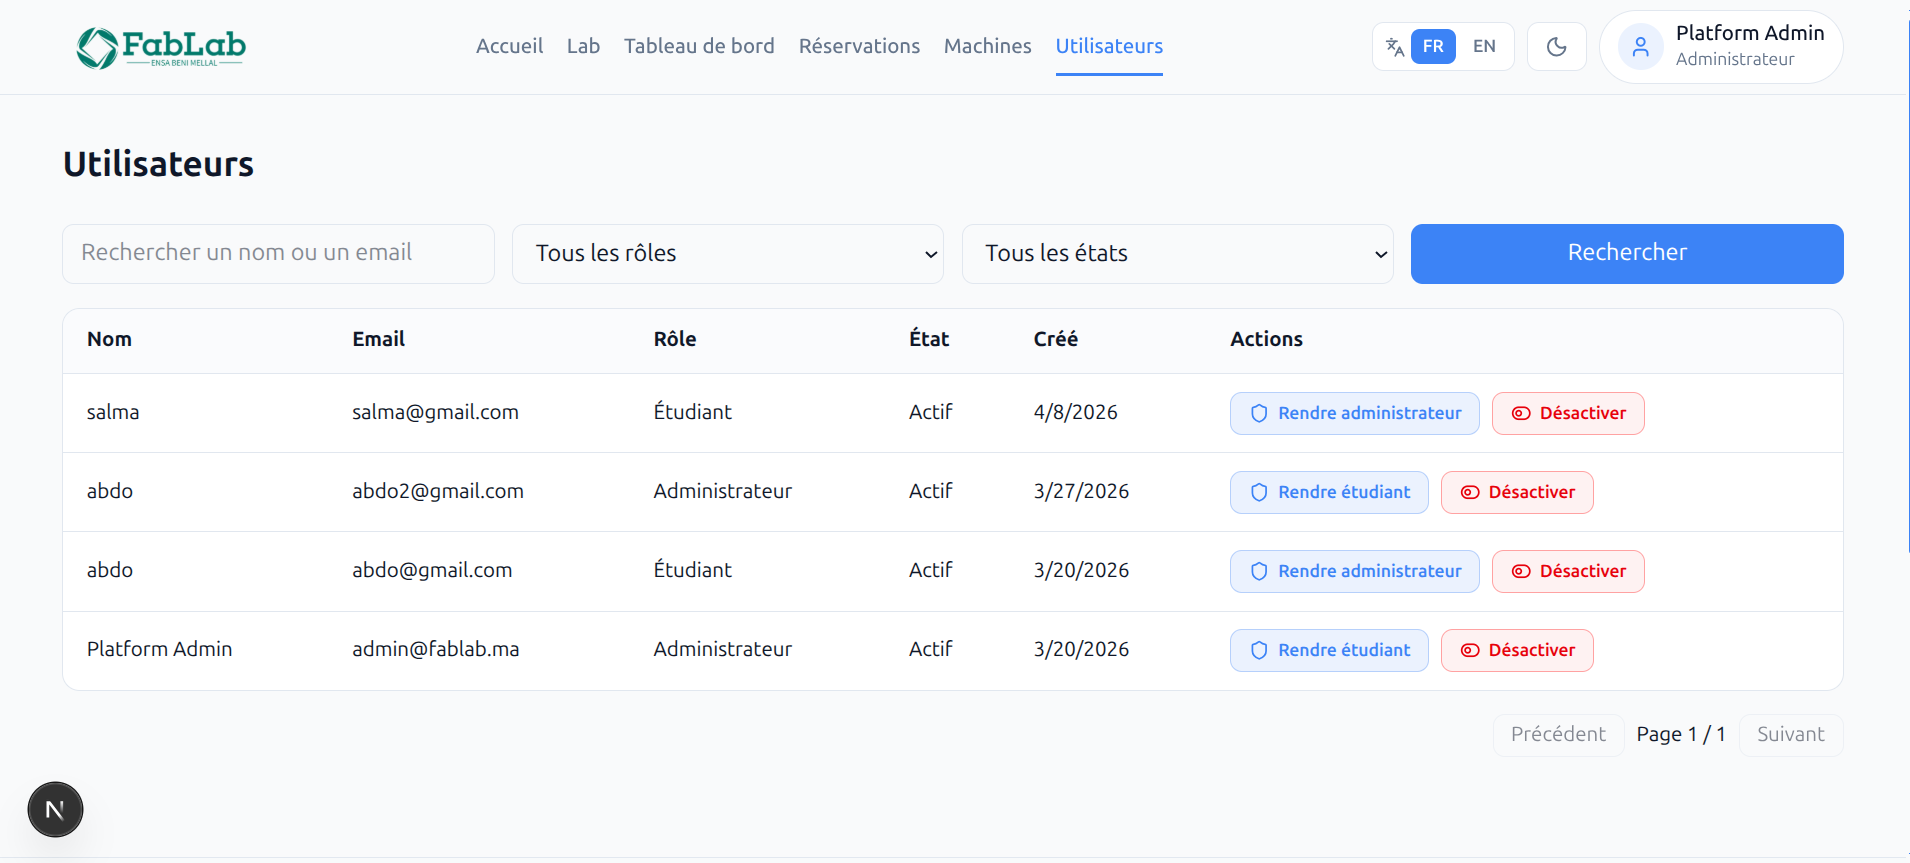
\includegraphics[width=0.95\textwidth]{images/screenshot_users_admin.png}}
{\fbox{\parbox[c][5cm][c]{0.85\textwidth}{\centering Emplacement réservé pour la gestion des utilisateurs\\\texttt{images/screenshot\_users\_admin.png}}}}
\caption{Interface de gestion des utilisateurs}
\label{fig:screenshot-users-admin}
\end{figure}

L’accès à ces fonctionnalités est protégé par une dépendance backend qui vérifie que l’utilisateur courant possède le rôle administrateur.

\section{Gestion des machines}

Le module machines permet de gérer les instances du FabLab. Chaque machine possède un type, un nom, un état, des notes et des paramètres de placement dans la scène 3D : position, rotation et échelle.

Les types de machines initialisés par défaut incluent notamment :

\begin{itemize}
    \item une imprimante 3D associée au modèle \texttt{/models/3d\_printer.glb} ;
    \item une machine CNC associée au modèle \texttt{/models/CNC.glb} ;
\end{itemize}

\begin{figure}[H]
\centering
\IfFileExists{images/screenshot_machines_admin.png}
{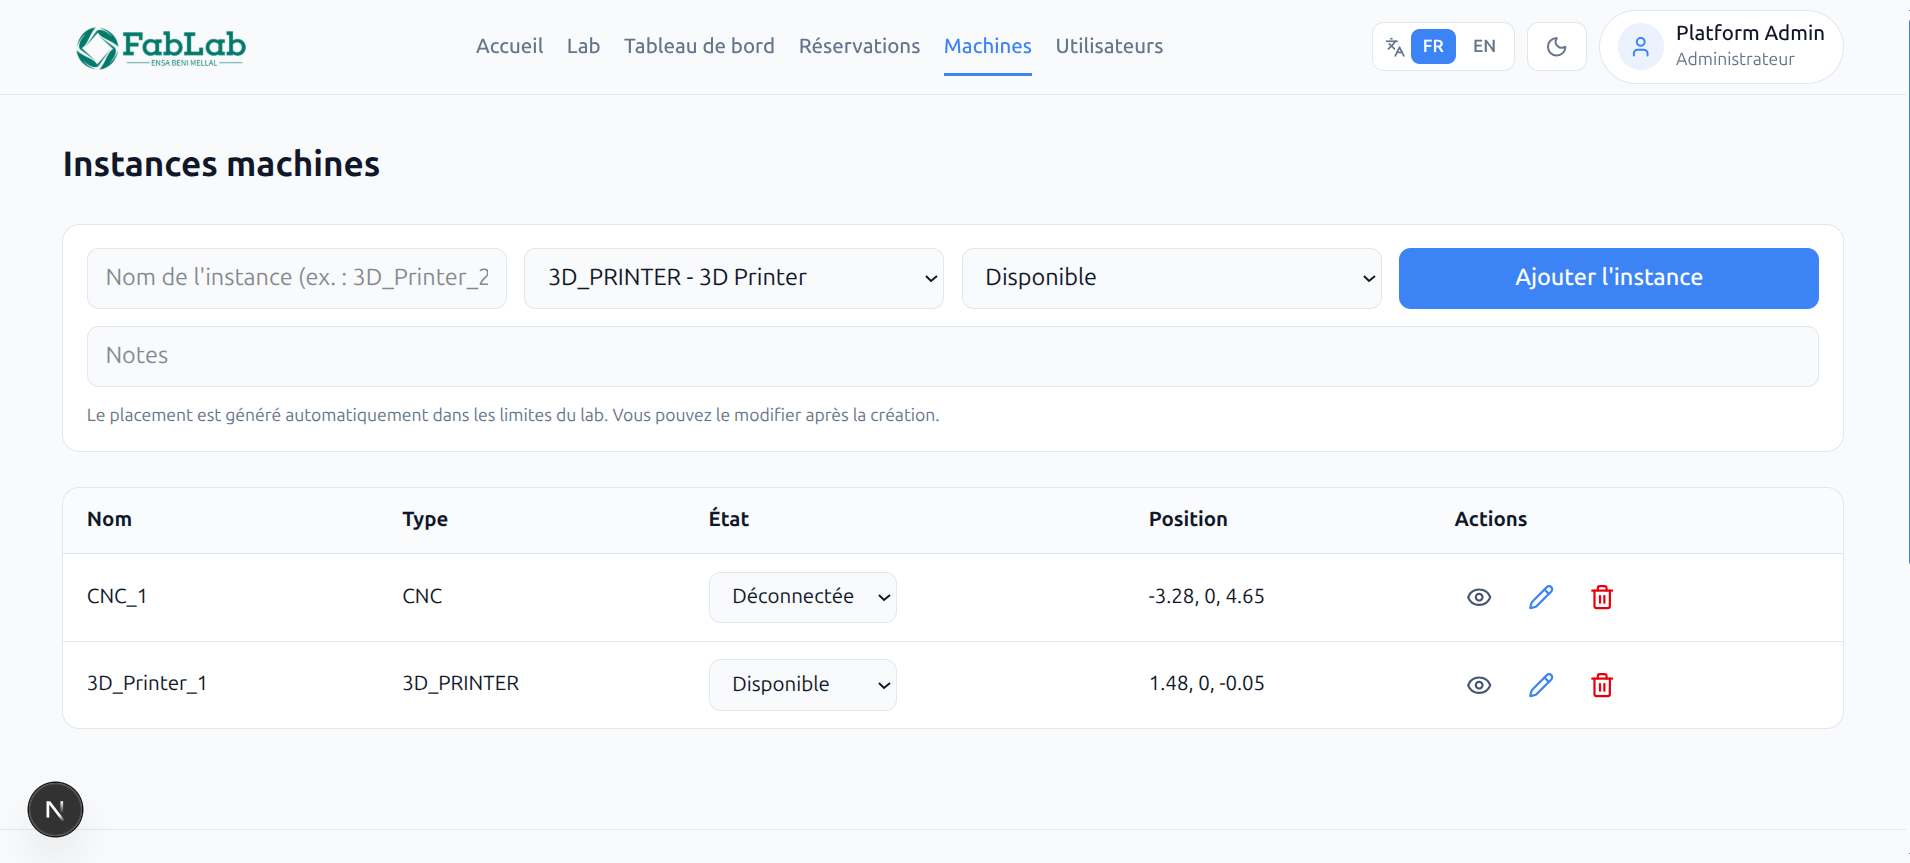
\includegraphics[width=0.95\textwidth]{images/screenshot_machines_admin.png}}
{\fbox{\parbox[c][5cm][c]{0.85\textwidth}{\centering Emplacement réservé pour l’interface de gestion des machines\\\texttt{images/screenshot\_machines\_admin.png}}}}
\caption{Interface de gestion des machines}
\label{fig:screenshot-machines-admin}
\end{figure}

\section{Système de réservation}

Le système de réservation permet à l’étudiant de choisir une machine, une date et un créneau horaire. Les créneaux sont générés entre 8h00 et 20h00 avec une durée d’une heure. Le backend vérifie les conflits afin d’empêcher deux réservations actives sur la même machine et le même intervalle.

Une demande de réservation est créée avec l’état \texttt{pending}. L’administrateur peut ensuite approuver ou refuser cette demande. Lorsqu’une décision est prise, une notification est créée pour l’utilisateur concerné.

\begin{figure}[H]
\centering
\IfFileExists{images/screenshot_reservations.png}
{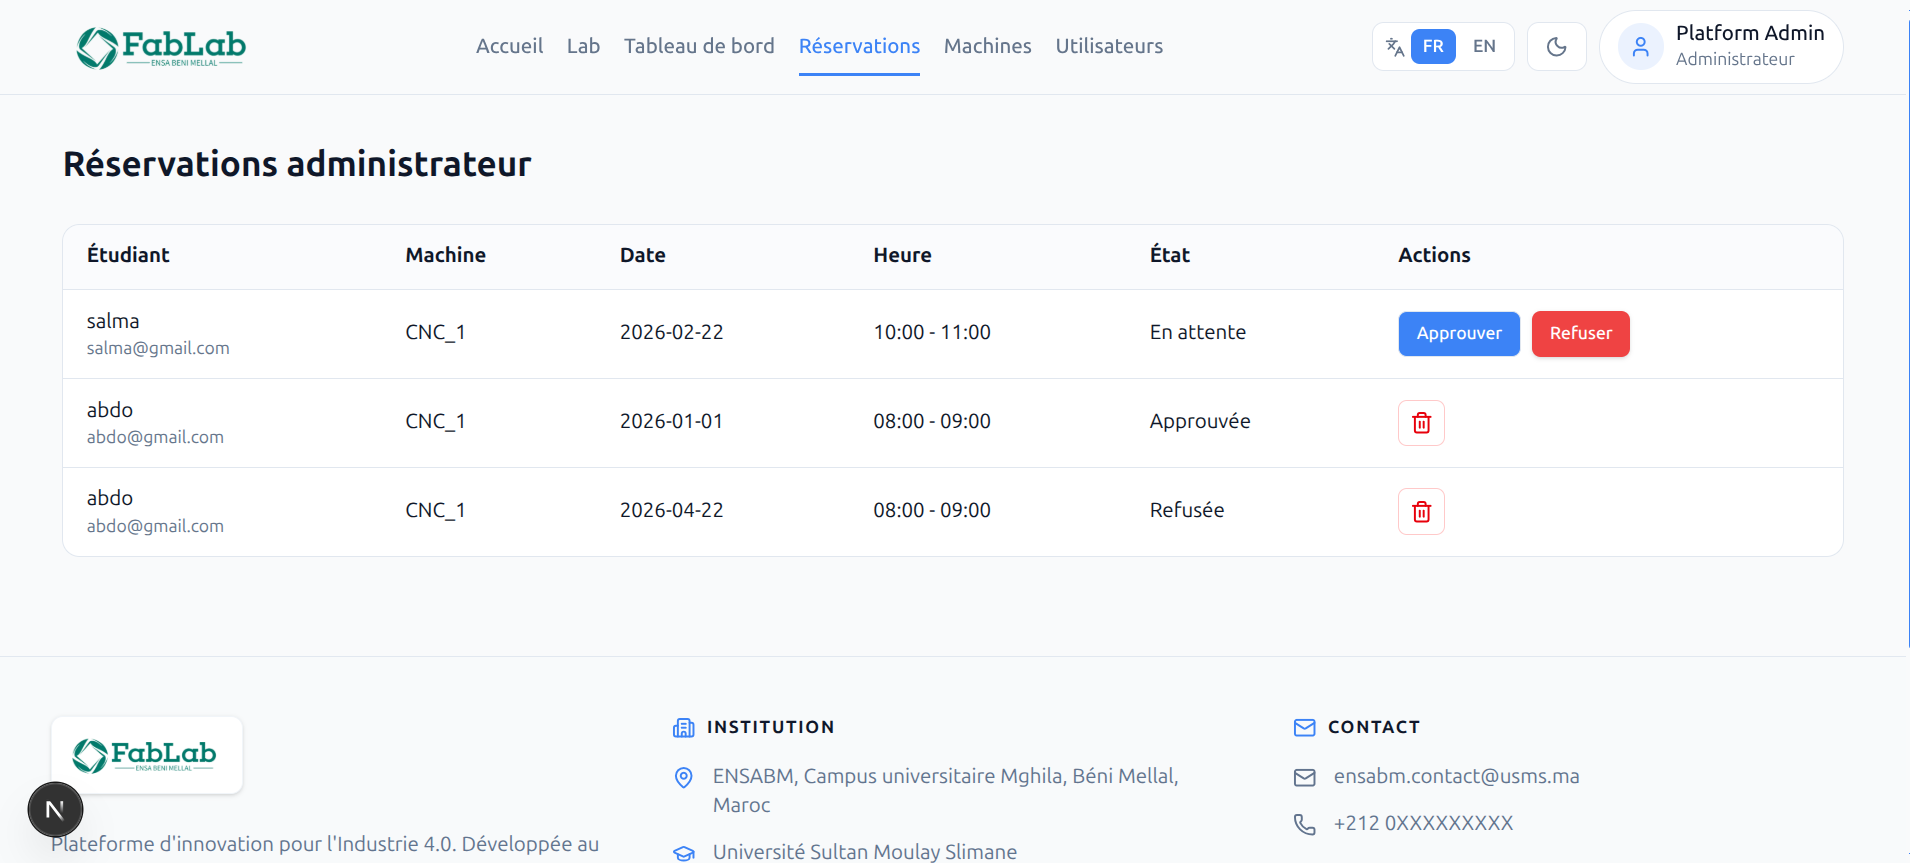
\includegraphics[width=0.95\textwidth]{images/screenshot_reservations.png}}
{\fbox{\parbox[c][5cm][c]{0.85\textwidth}{\centering Emplacement réservé pour l’interface de réservation\\\texttt{images/screenshot\_reservations.png}}}}
\caption{Interface de réservation des machines}
\label{fig:screenshot-reservations}
\end{figure}

\section{FabLab virtuel en 3D}

La page du laboratoire virtuel affiche une scène 3D représentant l’espace du FabLab. Les machines sont chargées dynamiquement depuis le backend, ce qui permet d’afficher les machines réellement enregistrées dans la base de données.

Chaque machine possède un modèle GLB, une position, une rotation et une échelle. L’utilisateur peut sélectionner une machine dans la scène afin de consulter son état, ses mesures récentes et ses actions disponibles : consulter les détails, ouvrir la simulation ou réserver.

\begin{figure}[H]
\centering
\IfFileExists{images/screenshot_lab_3d.png}
{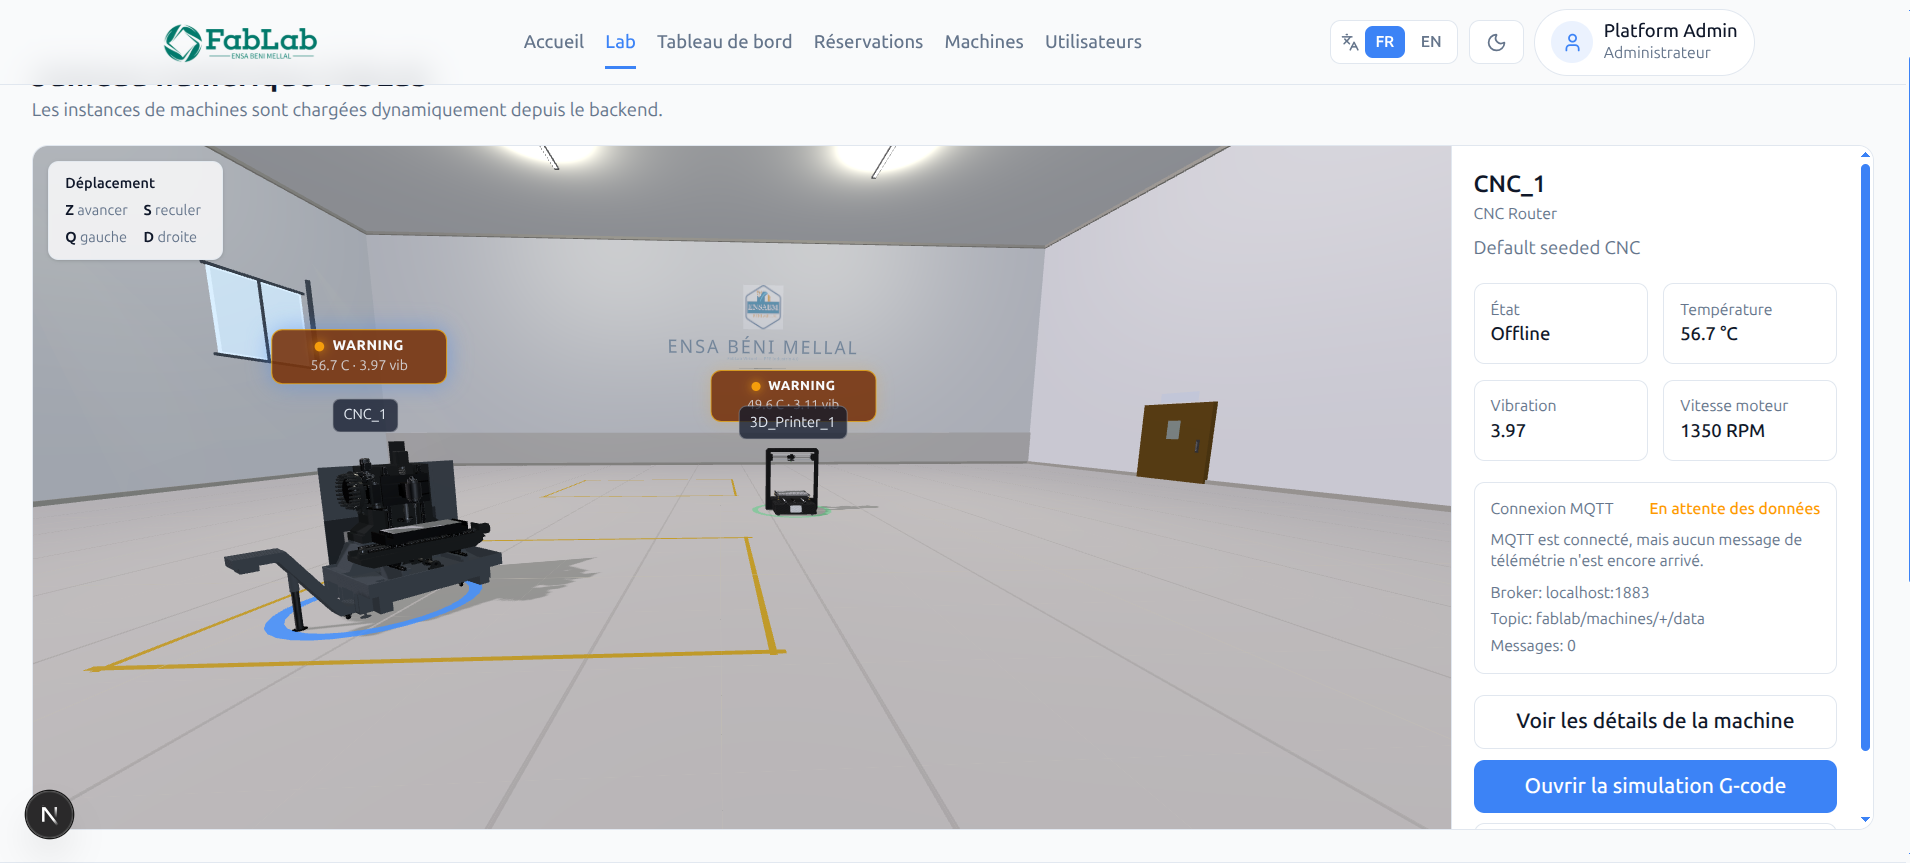
\includegraphics[width=0.95\textwidth]{images/screenshot_lab_3d.png}}
{\fbox{\parbox[c][5.5cm][c]{0.85\textwidth}{\centering Emplacement réservé pour la scène du FabLab virtuel\\\texttt{images/screenshot\_lab\_3d.png}}}}
\caption{Vue 3D du FabLab virtuel}
\label{fig:screenshot-lab-3d}
\end{figure}

\section{Simulation CNC}

La simulation CNC repose sur l’interprétation de fichiers NC ou G-code adaptés à une machine de fraisage ou de découpe. Le module détecte les commandes de mouvement, les vitesses d’avance, les arcs, les commandes de broche et certains signaux caractéristiques de la CNC.

Les trajectoires sont transformées en mouvements simulables dans la scène 3D. Les déplacements rapides et les opérations de coupe sont représentés différemment afin de distinguer les phases de positionnement et les phases d’usinage.

\begin{figure}[H]
\centering
\IfFileExists{images/screenshot_cnc_simulation.png}
{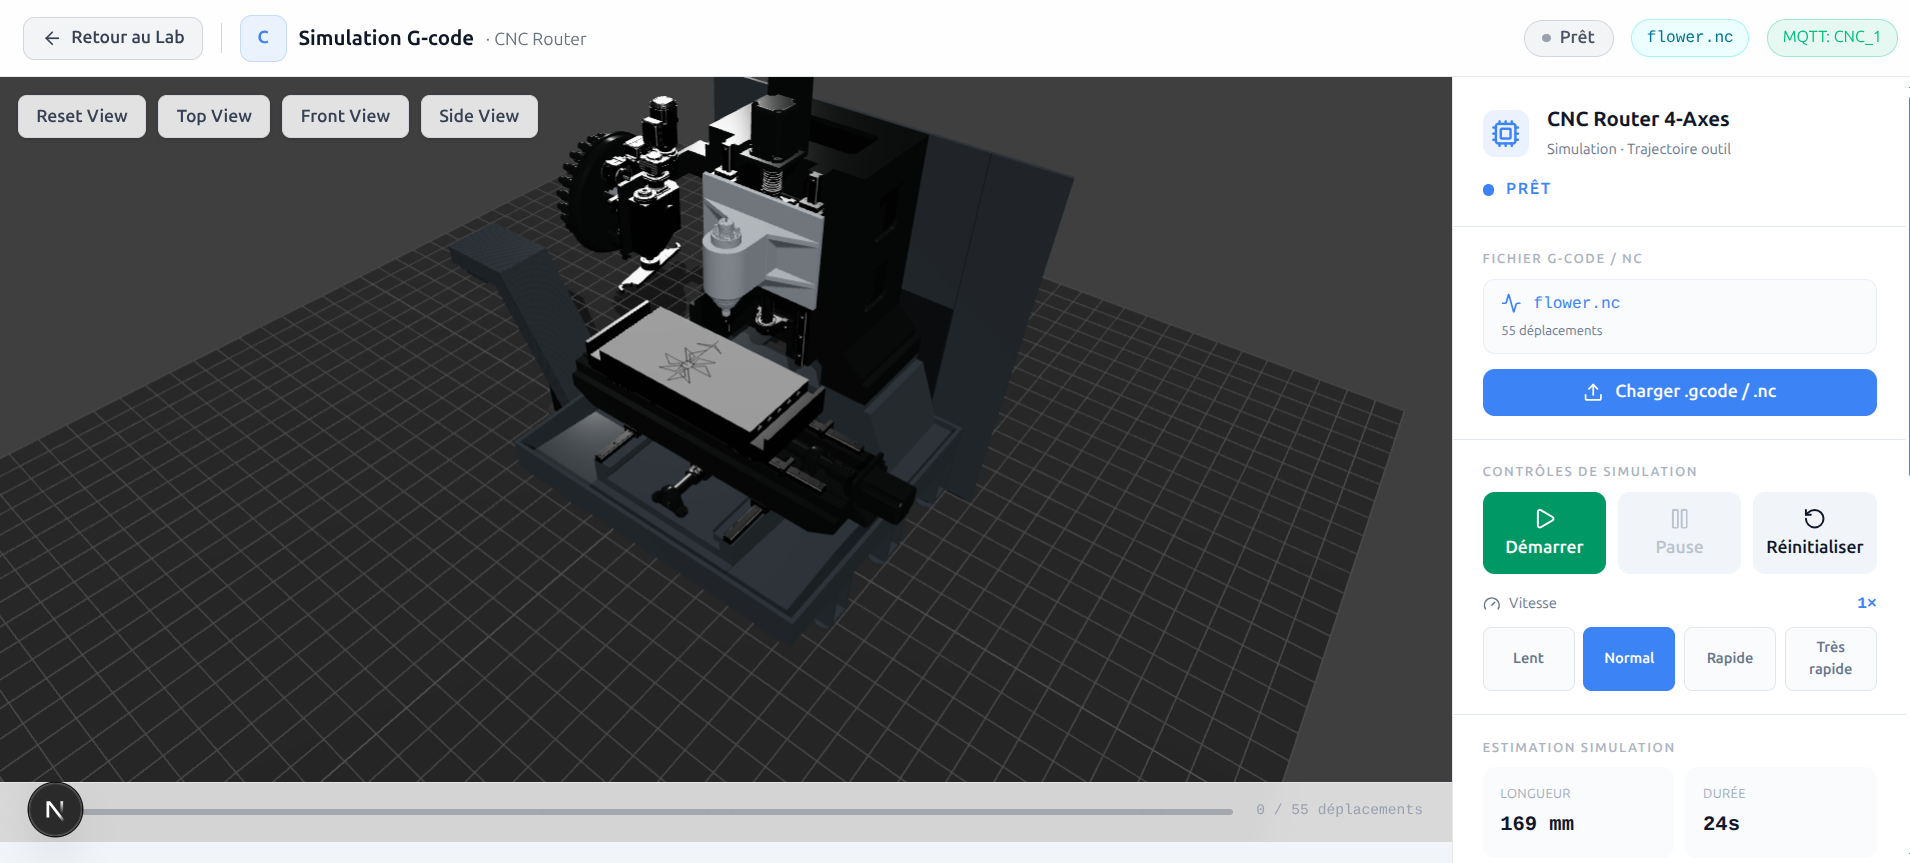
\includegraphics[width=0.95\textwidth]{images/screenshot_cnc_simulation.png}}
{\fbox{\parbox[c][5cm][c]{0.85\textwidth}{\centering Emplacement réservé pour la simulation CNC\\\texttt{images/screenshot\_cnc\_simulation.png}}}}
\caption{Simulation d’une trajectoire CNC}
\label{fig:screenshot-cnc-simulation}
\end{figure}

\section{Simulation de l’imprimante 3D}

La simulation de l’imprimante 3D prend en charge les fichiers G-code contenant les déplacements, l’axe d’extrusion, les vitesses d’avance et certaines commandes propres à l’impression 3D. Le système distingue les déplacements sans extrusion des segments imprimés.

La scène affiche progressivement la trajectoire d’impression et peut représenter les couches de l’objet. Le panneau latéral permet de suivre la progression, la position courante, la vitesse de lecture, la température simulée et les informations associées à la télémétrie lorsque la machine sélectionnée est liée à une instance enregistrée dans le backend.

\begin{figure}[H]
\centering
\IfFileExists{images/screenshot_printer_simulation.png}
{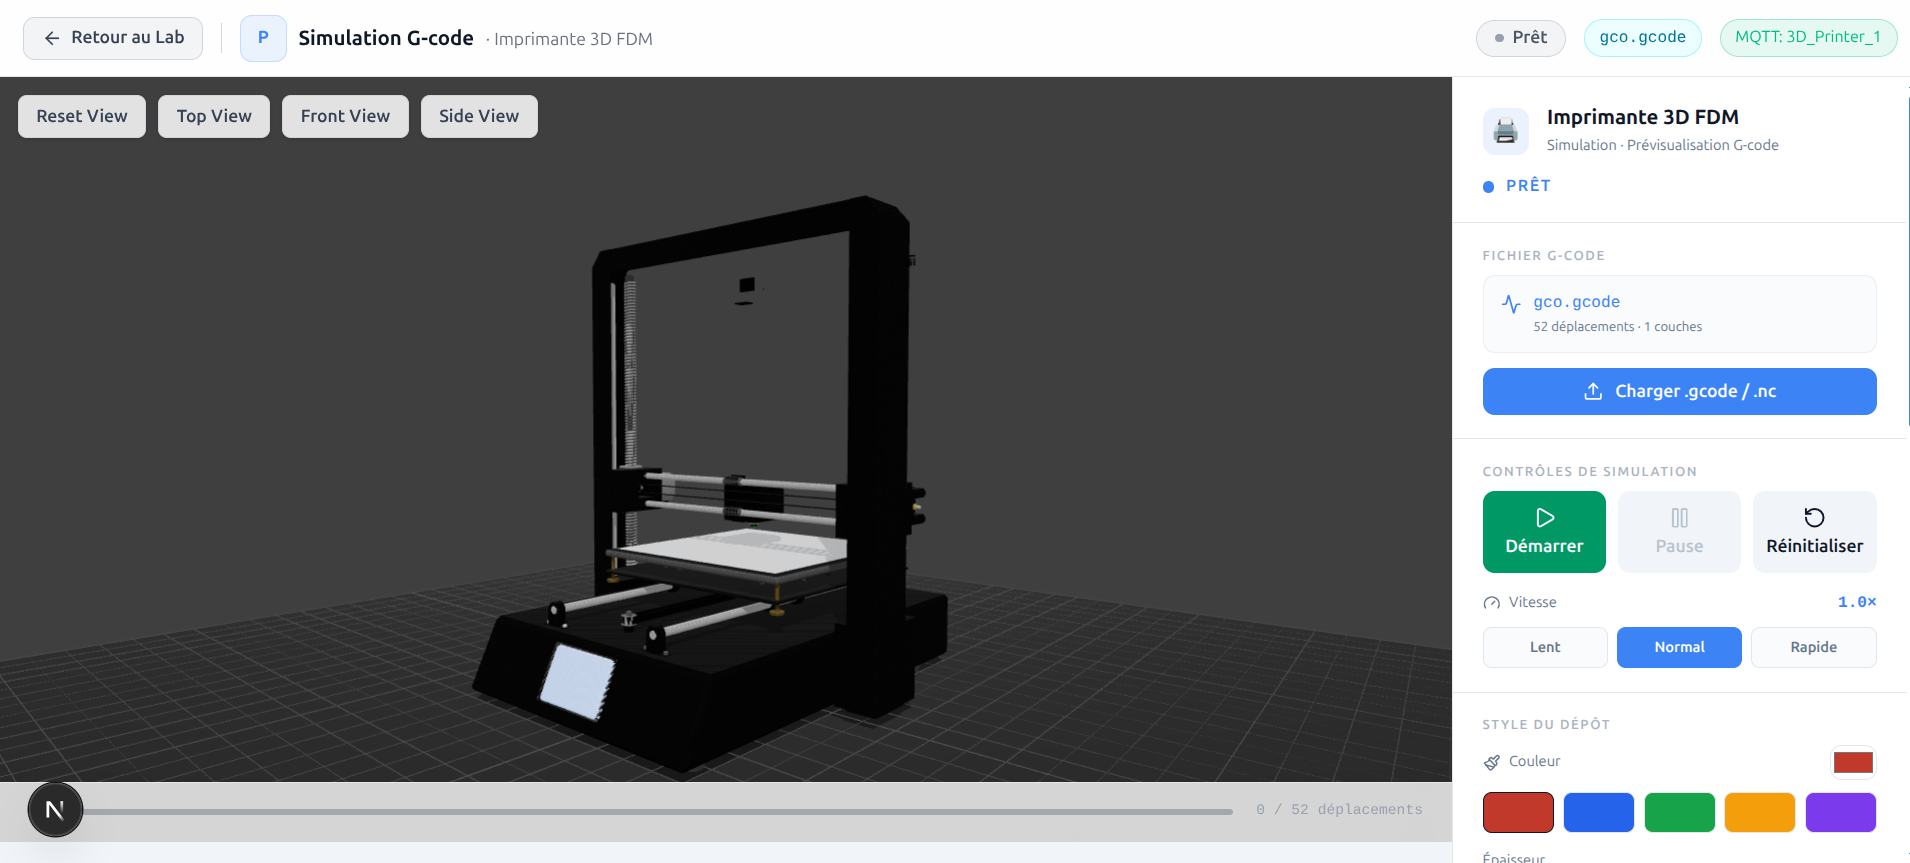
\includegraphics[width=0.95\textwidth]{images/screenshot_printer_simulation.png}}
{\fbox{\parbox[c][5cm][c]{0.85\textwidth}{\centering Emplacement réservé pour la simulation de l’imprimante 3D\\\texttt{images/screenshot\_printer\_simulation.png}}}}
\caption{Simulation d’un fichier G-code pour imprimante 3D}
\label{fig:screenshot-printer-simulation}
\end{figure}

\section{Interprétation des fichiers G-code et NC}

L’interprétation des fichiers est réalisée côté frontend afin de fournir un retour immédiat à l’utilisateur. Les lignes sont normalisées, les commentaires sont ignorés et les tokens de type \texttt{G}, \texttt{M}, \texttt{X}, \texttt{Y}, \texttt{Z}, \texttt{F}, \texttt{E}, \texttt{I}, \texttt{J} ou \texttt{R} sont analysés.

Le système vérifie également la compatibilité du fichier avec la machine sélectionnée. Par exemple, un fichier contenant des commandes de broche ou de refroidissement est considéré comme non compatible avec l’imprimante 3D, tandis qu’un fichier contenant des commandes d’extrusion est rejeté pour la CNC.

\begin{figure}[H]
\centering
\IfFileExists{images/gcode_validation_flow.png}
{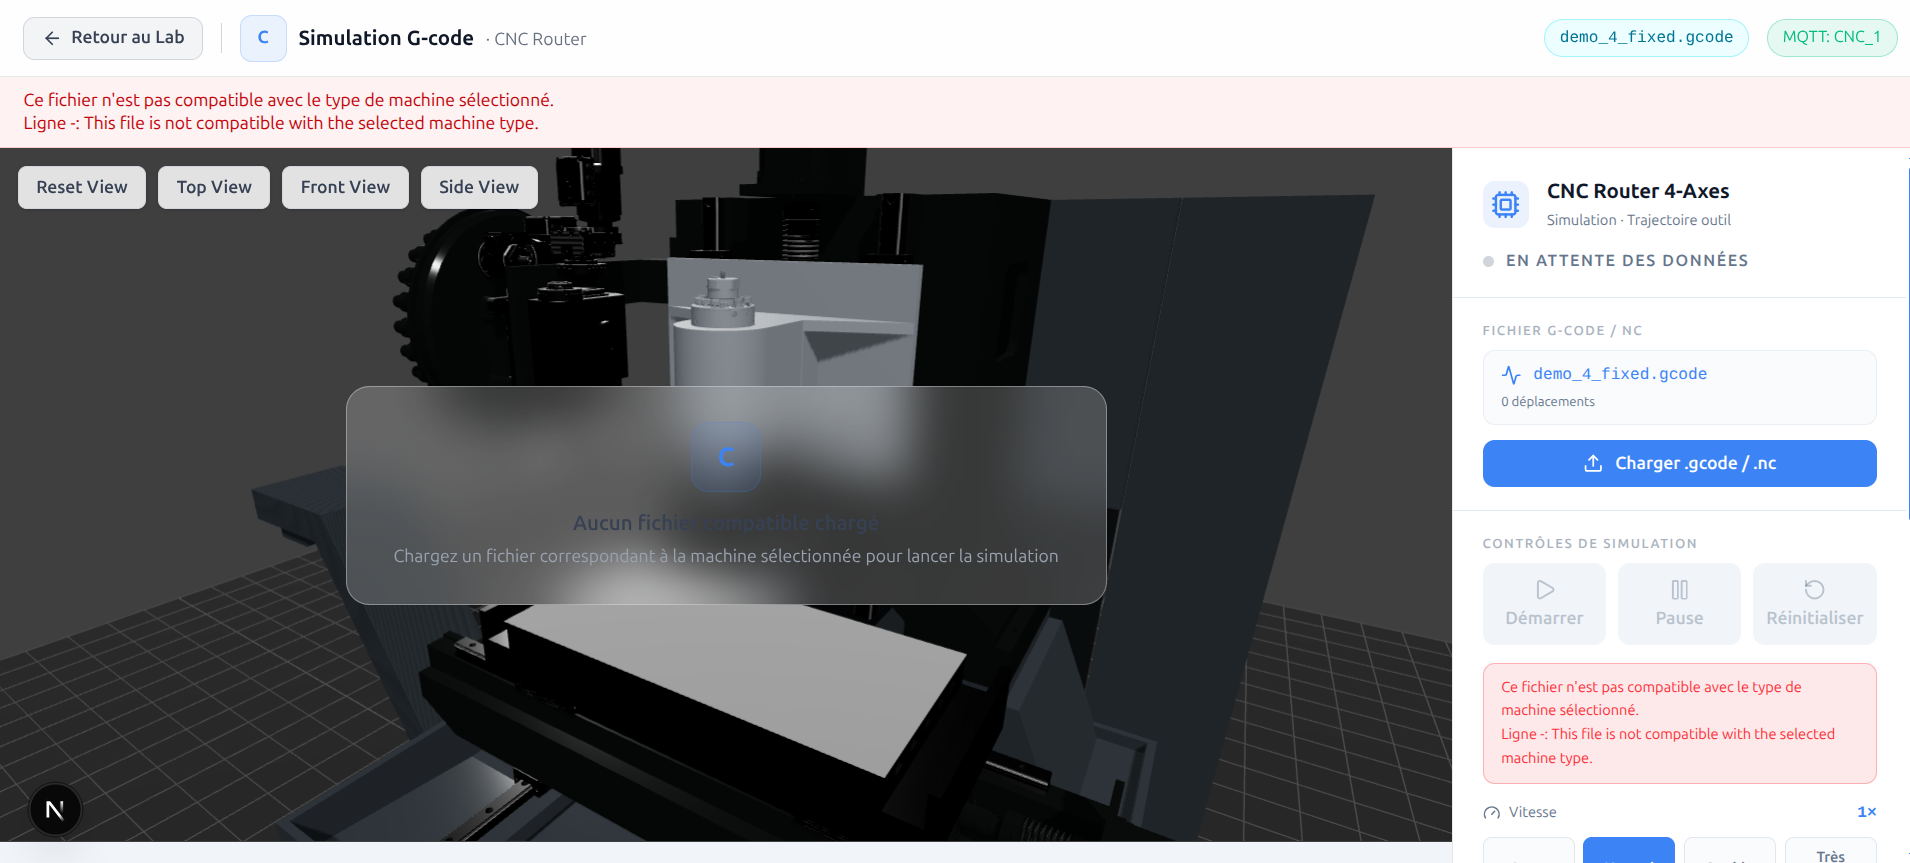
\includegraphics[width=0.9\textwidth]{images/gcode_validation_flow.png}}
{\fbox{\parbox[c][5cm][c]{0.85\textwidth}{\centering Emplacement réservé pour le processus d’interprétation G-code/NC\\\texttt{images/gcode\_validation\_flow.png}}}}
\caption{Processus d’interprétation et de validation des fichiers G-code/NC}
\label{fig:gcode-validation-flow}
\end{figure}

\section{Télémétrie simulée avec MQTT}

La télémétrie est simulée par un script Python qui publie périodiquement des messages MQTT. Ce choix permet de valider le flux complet sans dépendre, à ce stade, d’une installation physique de capteurs. Les données utilisées dans cette version sont simulées afin de valider l’architecture, les flux MQTT, le monitoring et le module d’analyse. La plateforme reste conçue pour être connectée ultérieurement à des capteurs réels. Chaque message est envoyé sur un topic de la forme :

\begin{center}
\texttt{fablab/machines/\{machine\_id\}/data}
\end{center}

Le message contient l’identifiant de la machine, la température, la vibration, la durée d’utilisation, la vitesse du moteur, une éventuelle erreur et un horodatage. Le backend s’abonne au motif \texttt{fablab/machines/+/data}, analyse les messages JSON et enregistre les mesures dans la base de données SQLite.

\begin{figure}[H]
\centering
\IfFileExists{images/mqtt_flow_real.png}
{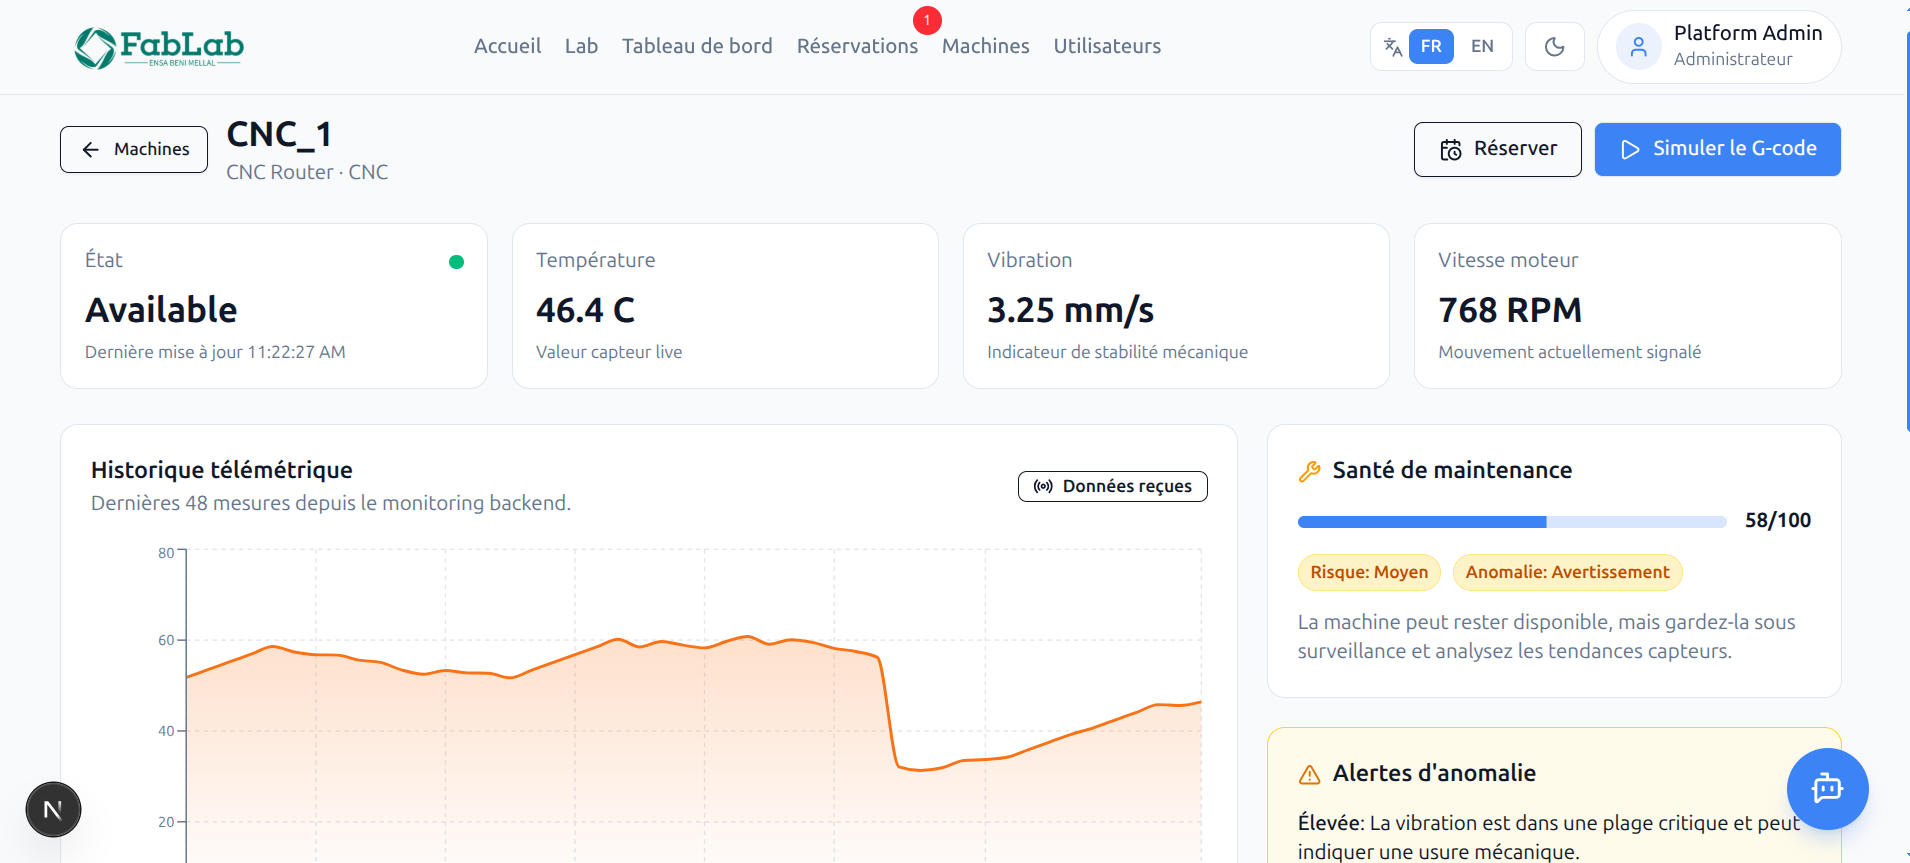
\includegraphics[width=0.95\textwidth]{images/mqtt_flow_real.png}}
{\fbox{\parbox[c][5cm][c]{0.85\textwidth}{\centering Emplacement réservé pour le flux MQTT implémenté\\\texttt{images/mqtt\_flow\_real.png}}}}
\caption{Flux MQTT implémenté dans la plateforme}
\label{fig:mqtt-flow-real}
\end{figure}

\section{Tableau de bord de supervision}

Le tableau de bord administrateur centralise les informations de supervision. Il affiche l’état de la connexion MQTT, la fraîcheur des données, le nombre d’utilisateurs, le nombre de machines, les réservations en attente et les résultats de monitoring intelligent.

Sur le plan de l’implémentation, le frontend interroge les endpoints administrateur du backend afin d’afficher les résultats calculés par les services d’analyse. Les éléments restitués incluent notamment :

\begin{itemize}
    \item un statut d’anomalie par machine ;
    \item un score de santé sur 100 ;
    \item un niveau de risque de maintenance ;
    \item une probabilité indicative de risque ;
    \item une recommandation de maintenance ;
    \item des facteurs explicatifs tels que température, vibration, durée d’utilisation, vitesse du moteur et erreurs récentes.
\end{itemize}

Les principes scientifiques, les caractéristiques utilisées, les modèles Machine Learning et les limites de validation sont détaillés dans le chapitre suivant afin d’éviter la duplication entre l’implémentation logicielle et la contribution analytique.

\begin{figure}[H]
\centering
\IfFileExists{images/screenshot_dashboard_ds.png}
{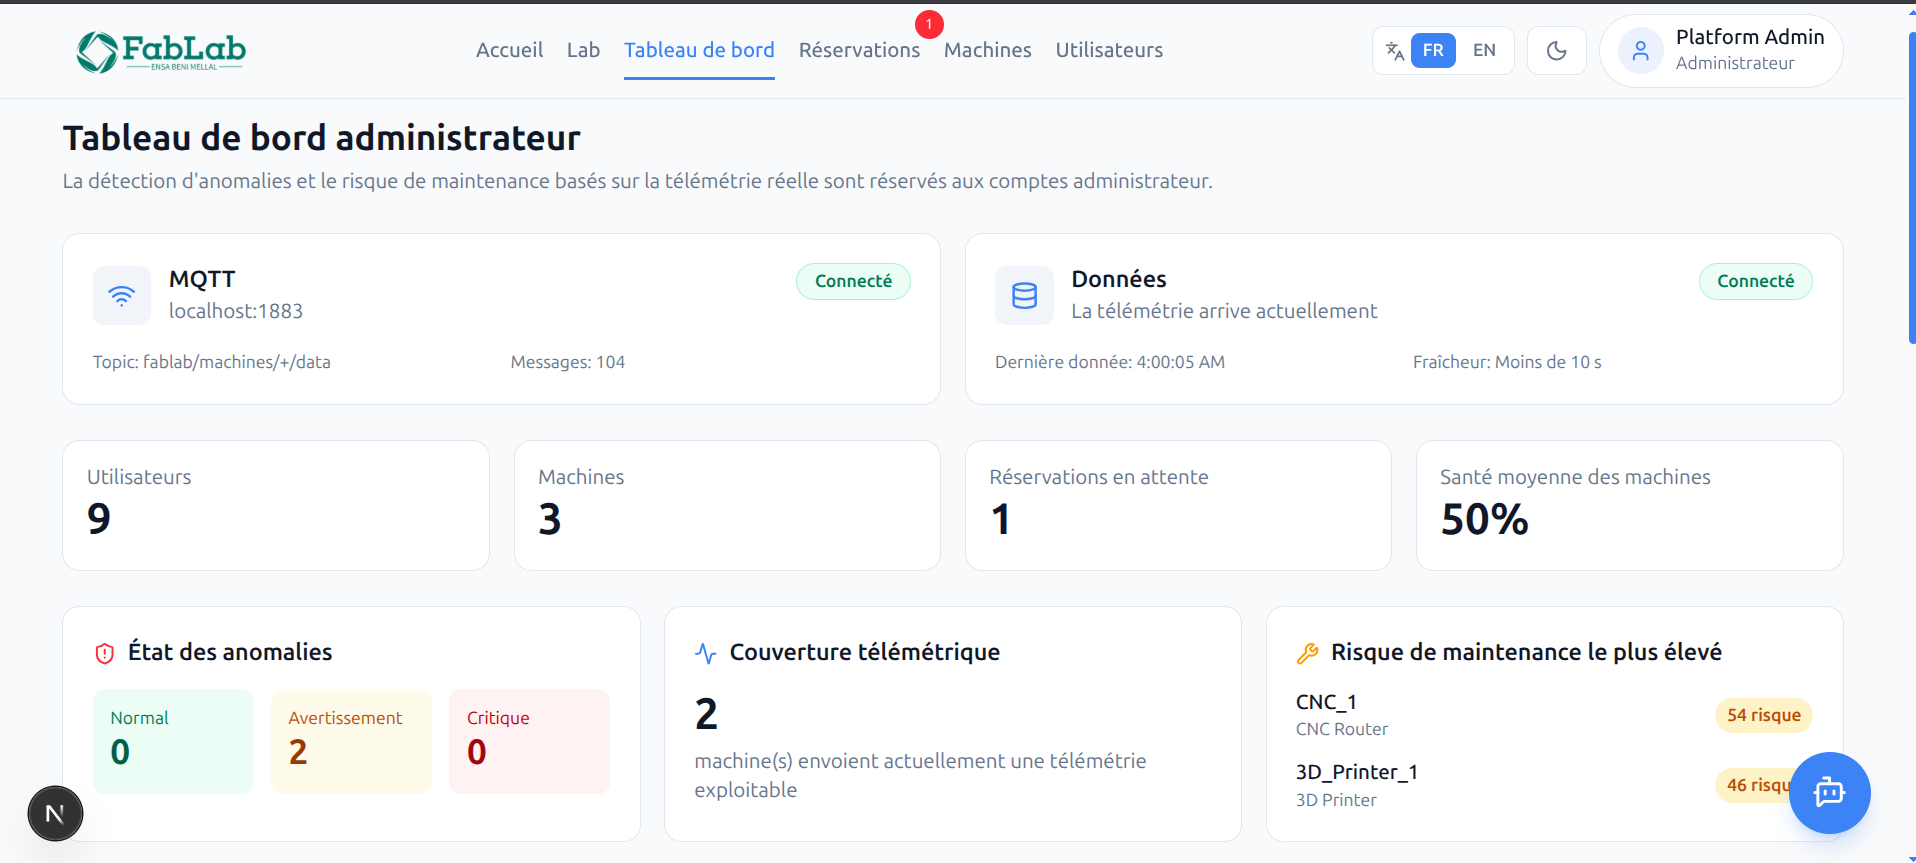
\includegraphics[width=0.95\textwidth]{images/screenshot_dashboard_ds.png}}
{\fbox{\parbox[c][5.5cm][c]{0.85\textwidth}{\centering Emplacement réservé pour le tableau de bord Data Science\\\texttt{images/screenshot\_dashboard\_ds.png}}}}
\caption{Tableau de bord administrateur et supervision intelligente}
\label{fig:screenshot-dashboard-ds}
\end{figure}

\section{Cartes de prédiction et historique de télémétrie}

Les cartes de prédiction du tableau de bord permettent de consulter rapidement les machines présentant un besoin de surveillance. Elles affichent les résultats déjà calculés par le backend : score de santé, probabilité indicative, niveau de risque et recommandation synthétique. Cette partie relève de l’intégration applicative, tandis que le détail des modèles est présenté séparément dans le chapitre consacré au module Data Science et IA.

\begin{figure}[H]
\centering
\IfFileExists{images/screenshot_prediction_cards.png}
{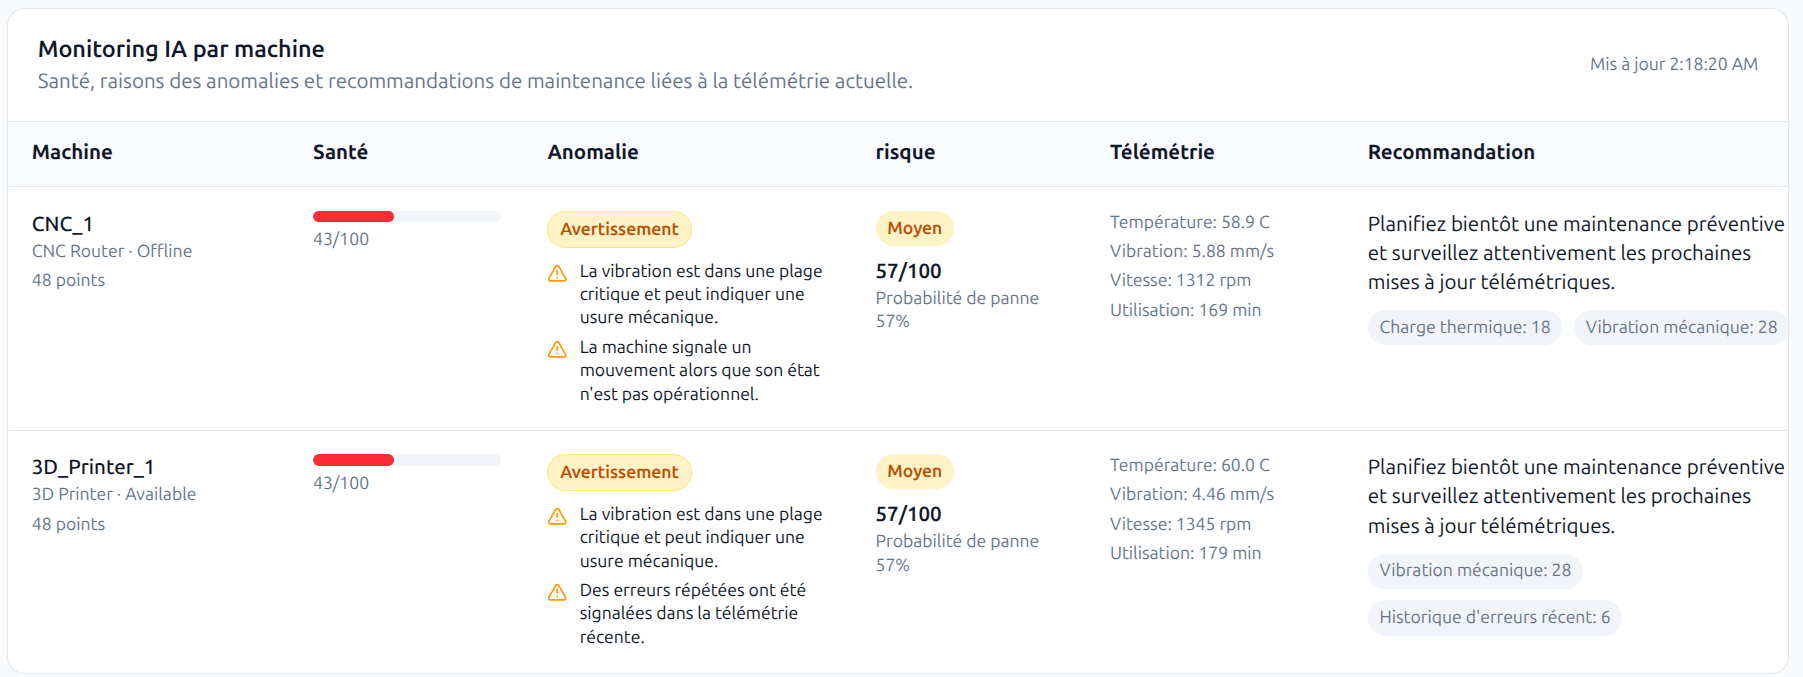
\includegraphics[width=0.95\textwidth]{images/screenshot_prediction_cards.png}}
{\fbox{\parbox[c][5cm][c]{0.85\textwidth}{\centering Emplacement réservé pour les cartes de prédiction\\\texttt{images/screenshot\_prediction\_cards.png}}}}
\caption{Cartes de prédiction et score de santé des machines}
\label{fig:screenshot-prediction-cards}
\end{figure}

Les pages de détail des machines exploitent l’historique des mesures stockées pour afficher l’évolution de certains indicateurs, notamment la température. Cette visualisation permet à l’administrateur de suivre l’état récent d’une machine et de relier les alertes à une série temporelle.

\begin{figure}[H]
\centering
\IfFileExists{images/screenshot_telemetry_history.png}
{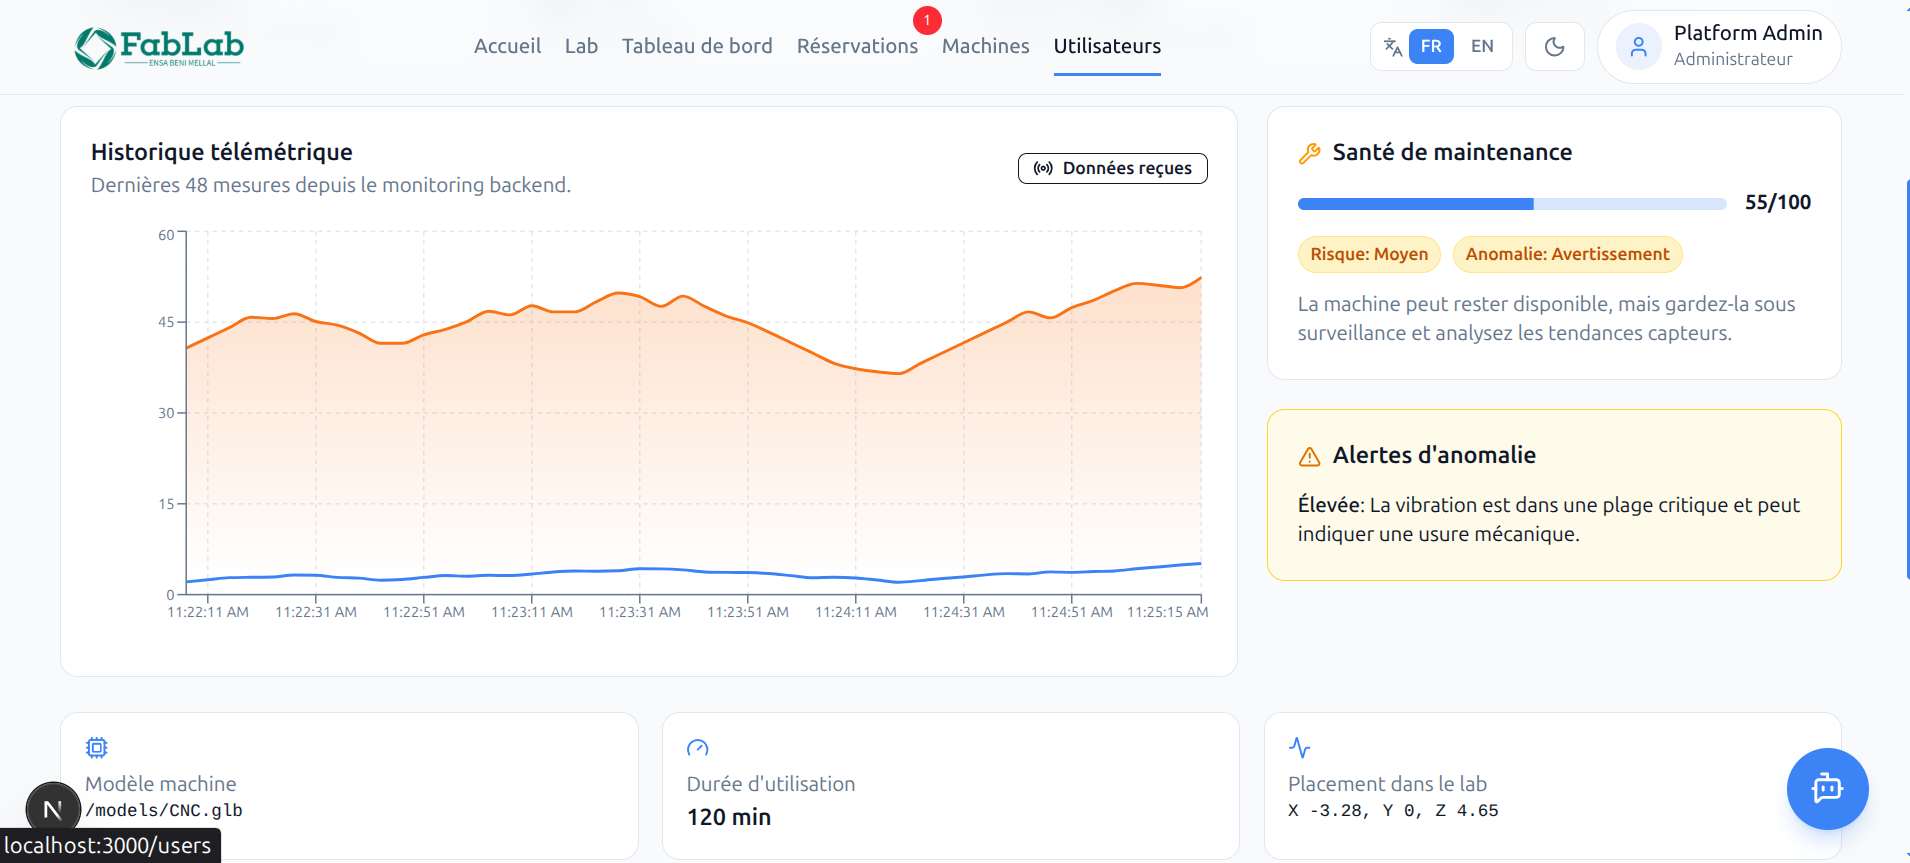
\includegraphics[width=0.95\textwidth]{images/screenshot_telemetry_history.png}}
{\fbox{\parbox[c][5cm][c]{0.85\textwidth}{\centering Emplacement réservé pour l’historique de télémétrie\\\texttt{images/screenshot\_telemetry\_history.png}}}}
\caption{Historique des mesures d’une machine}
\label{fig:screenshot-telemetry-history}
\end{figure}

\section{Intégration technique du Copilote IA}

L’espace administrateur intègre une interface flottante de type chatbot appelée Assistant IA de Maintenance. Cette interface est chargée dans le layout de l’application, mais elle n’est affichée que lorsque l’utilisateur connecté possède le rôle \texttt{admin}. Elle conserve l’historique de conversation localement dans l’état React du composant et envoie les questions au backend à travers l’endpoint \texttt{/admin/ai/copilot/query}.

Le frontend affiche la réponse structurée retournée par le backend : intention reconnue, niveau de sévérité, confiance, texte de synthèse, points de données et recommandations. Cette intégration fournit un accès conversationnel aux informations du tableau de bord, sans transformer le système en modèle génératif. Le fonctionnement scientifique du classifieur d’intentions et la génération déterministe des réponses sont détaillés dans le chapitre suivant.

\section{Communication entre frontend et backend}

La communication entre le frontend et le backend est centralisée dans une fonction utilitaire d’appel API. Cette fonction construit l’URL du backend, ajoute l’en-tête \texttt{Content-Type}, insère le jeton d’authentification lorsque nécessaire et traite les erreurs HTTP.

Cette couche simplifie l’usage des API dans les pages Next.js. Elle permet également de maintenir une cohérence dans la gestion des réponses, des erreurs et des routes protégées.

\begin{figure}[H]
\centering
\IfFileExists{images/api_communication.png}
{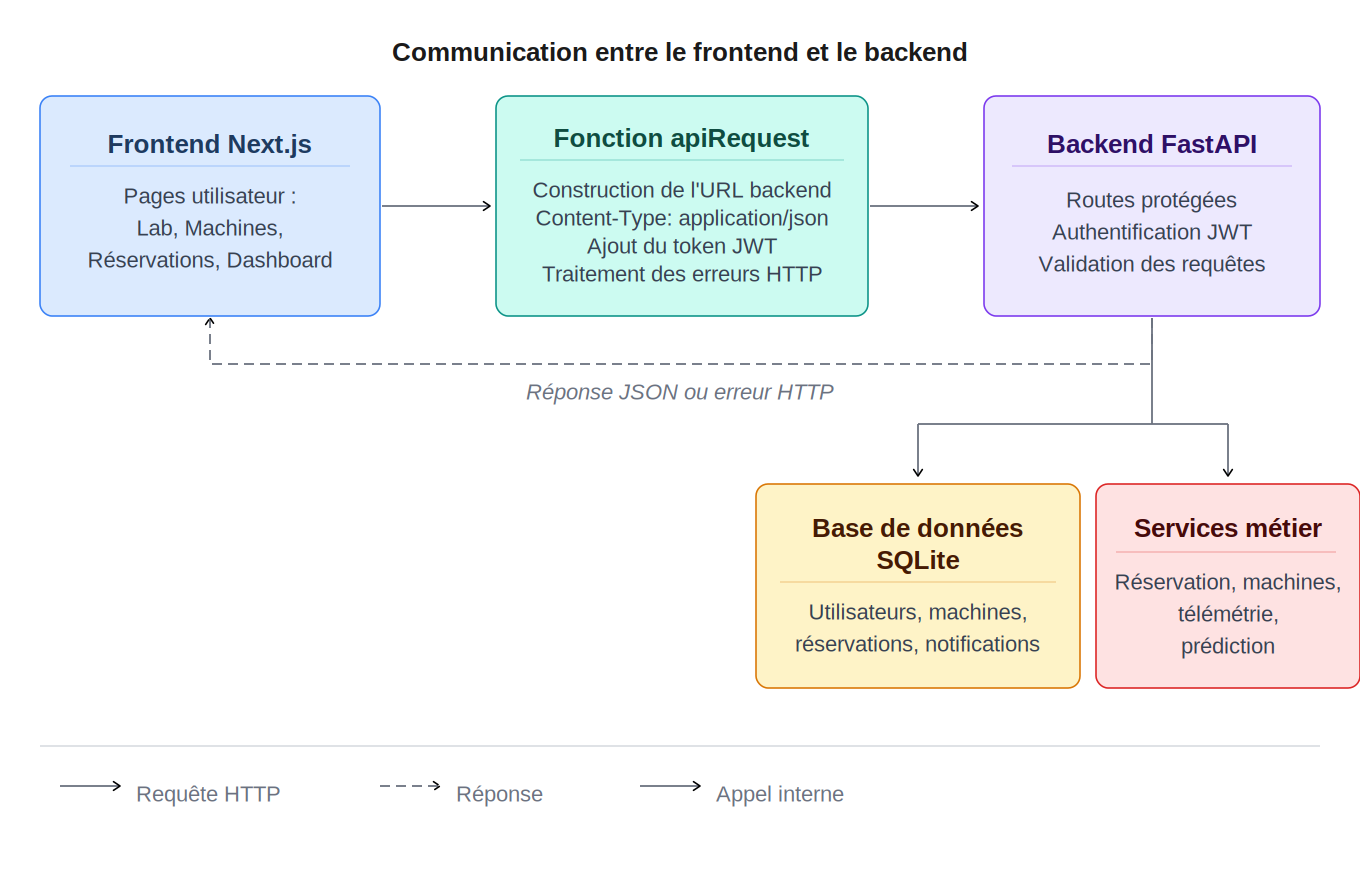
\includegraphics[width=0.9\textwidth]{images/api_communication.png}}
{\fbox{\parbox[c][5cm][c]{0.85\textwidth}{\centering Emplacement réservé pour le schéma de communication API\\\texttt{images/api\_communication.png}}}}
\caption{Communication entre le frontend et le backend}
\label{fig:api-communication}
\end{figure}

\section{Interfaces réalisées}

Les interfaces réalisées couvrent les principaux parcours utilisateurs : accueil, connexion, inscription, laboratoire 3D, simulation, réservation, profil, gestion des machines, gestion des utilisateurs, réservations administrateur et tableau de bord. Les captures présentées dans les sections précédentes illustrent les écrans les plus représentatifs de ces parcours.

\section{Conclusion}

Ce chapitre a présenté la réalisation technique de la plateforme Virtual FabLab. L’implémentation couvre la gestion des utilisateurs, des machines et des réservations, la visualisation du laboratoire en 3D, la simulation CNC et imprimante 3D, l’ingestion MQTT, le tableau de bord de supervision et l’intégration technique du Copilote IA.

Le chapitre suivant approfondira l’exploitation des données IoT et l’intégration de la Data Science et de l’IA, en détaillant les données utilisées, les modèles de détection, la classification d’intentions, les recommandations de maintenance et les limites de l’approche adoptée.

\chapter{Module Data Science et Intelligence Artificielle}

\section{Introduction}

Ce chapitre présente la contribution Data Science et Intelligence Artificielle intégrée à la plateforme \textbf{Virtual FabLab}. Contrairement au chapitre précédent, centré sur la réalisation logicielle, cette partie analyse la chaîne de traitement des données, les modèles utilisés, le classifieur d'intentions et le copilote d'aide à la décision réservé à l'administrateur.

Le module étudié repose sur des données de télémétrie simulées. Il ne constitue donc pas une validation industrielle de maintenance prédictive, mais un prototype académique permettant de démontrer l'intégration entre ingestion MQTT, stockage, apprentissage automatique, classification supervisée d'intentions et restitution des résultats dans l'interface d'administration.

\section{Architecture du module Data Science et IA}

Le module Data Science et IA est placé côté backend. Il reçoit les mesures stockées après ingestion MQTT, extrait les caractéristiques nécessaires, charge les modèles persistés avec \texttt{joblib}, puis produit des résultats structurés consommés par le tableau de bord et par le Copilote IA de maintenance.

\begin{figure}[H]
\centering
\IfFileExists{images/architecture_data_science_ia.png}
{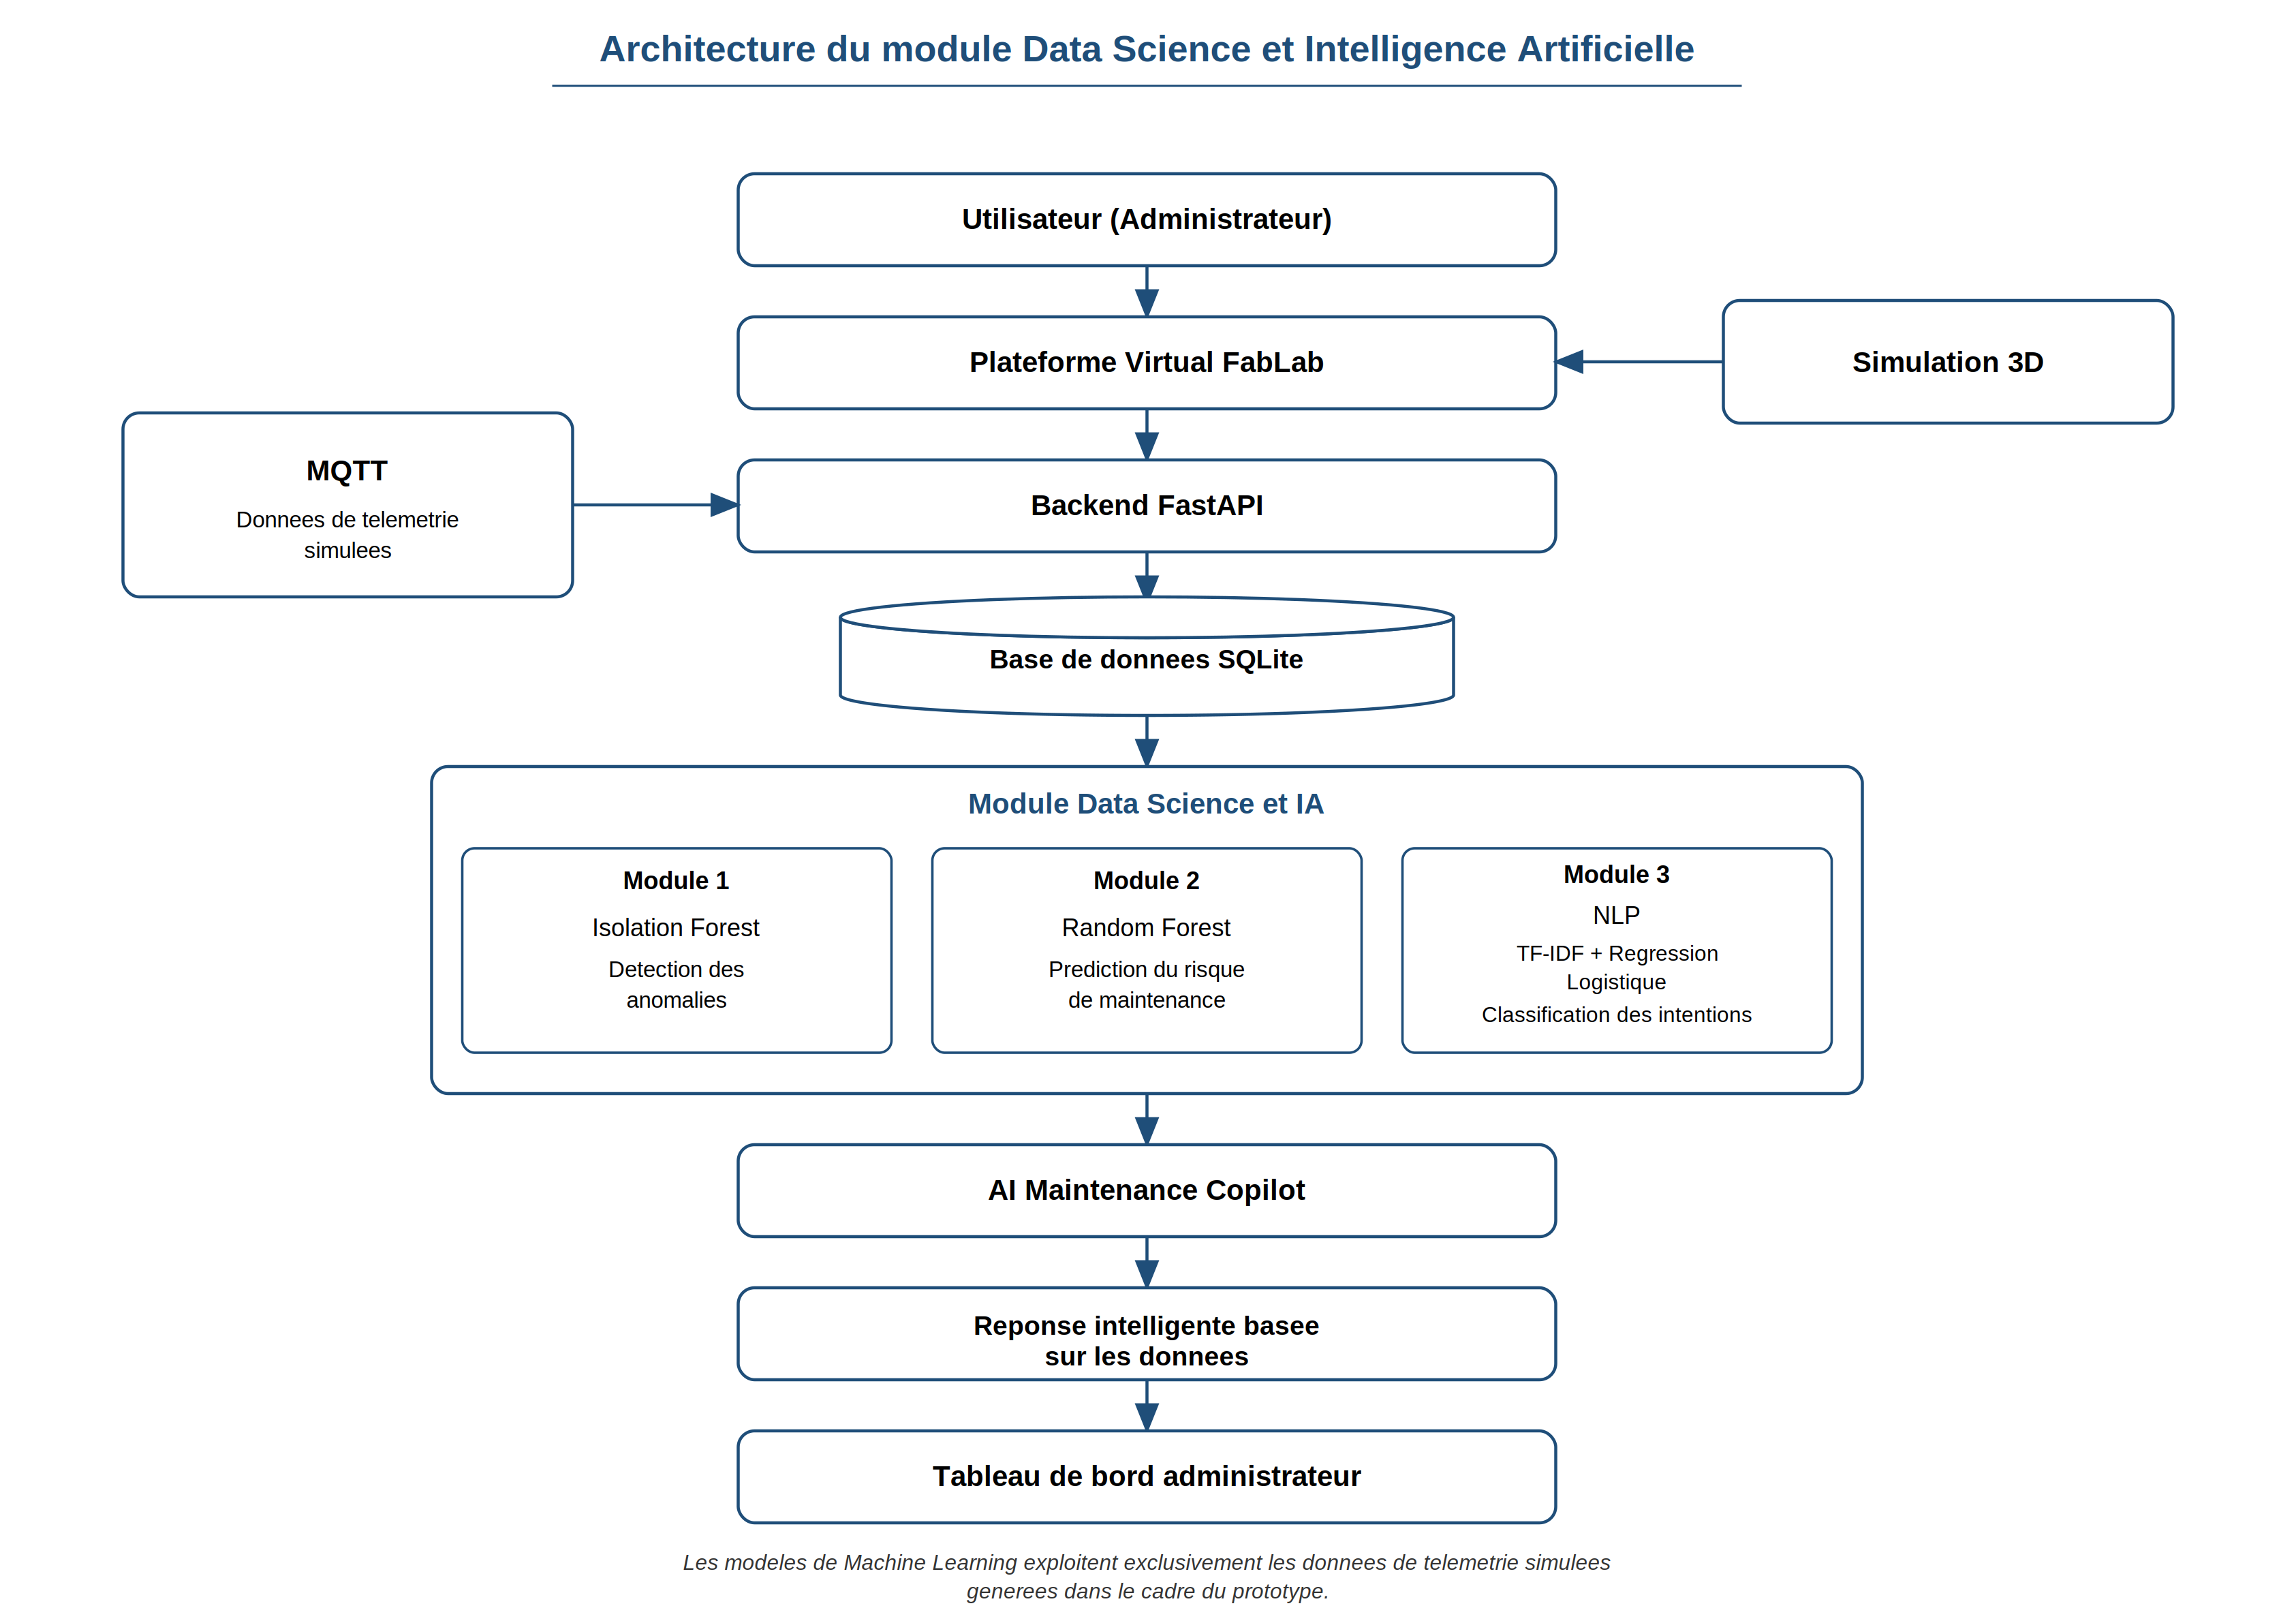
\includegraphics[width=0.95\textwidth]{images/architecture_data_science_ia.png}}
{\fbox{\parbox[c][5.8cm][c]{0.88\textwidth}{\centering Emplacement réservé pour le pipeline Data Science et IA\\[2mm]\texttt{images/architecture\_data\_science\_ia.png}\\[2mm]\small MQTT telemetry $\rightarrow$ database $\rightarrow$ preprocessing $\rightarrow$ feature engineering $\rightarrow$ Isolation Forest $\rightarrow$ Random Forest $\rightarrow$ health/risk outputs $\rightarrow$ dashboard and Copilot}}}
\caption{Pipeline Data Science et IA de la plateforme}
\label{fig:architecture-data-science-ia}
\end{figure}

La figure \ref{fig:architecture-data-science-ia} doit représenter le passage des messages MQTT vers la base de données, puis vers les traitements de prétraitement, d'ingénierie des caractéristiques, de détection d'anomalies, d'estimation du risque et de restitution dans le tableau de bord et le copilote.

\section{Collecte et nature des données}

Les données exploitées par le module proviennent d'un simulateur MQTT, et non de capteurs physiques connectés. Le script de simulation publie des messages JSON sur des topics propres à chaque machine, selon le motif suivant :

\begin{center}
\small\texttt{fablab/machines/\{machine\_id\}/data}
\end{center}

Le backend s'abonne au motif \texttt{fablab/machines/+/data}, parse les messages reçus et enregistre les mesures dans la table des lectures capteurs.

Les champs effectivement exploités sont la température, la vibration, la durée d'utilisation, la vitesse du moteur, l'erreur éventuelle et l'horodatage. La durée d'utilisation est reçue sous forme de \texttt{usage\_duration}, puis convertie en heures pour les modèles. La présence d'une erreur est transformée en variable binaire.

\begin{table}[H]
\centering
\small
\caption{Nature des données utilisées par le module Data Science}
\label{tab:donnees-ds-ia}
\begin{tabular}{|p{0.24\textwidth}|p{0.22\textwidth}|p{0.44\textwidth}|}
\hline
\rowcolor{SectionColor!12}
\textbf{Donnée} & \textbf{Origine} & \textbf{Utilisation} \\
\hline
\texttt{temperature} & MQTT simulé & Détection de dérive thermique, score de risque et facteurs explicatifs. \\
\hline
\texttt{vibration} & MQTT simulé & Détection de vibration anormale et estimation du risque. \\
\hline
\texttt{motor\_speed} & MQTT simulé & Contrôle de cohérence et contribution au risque. \\
\hline
\texttt{usage\_duration} & MQTT simulé & Conversion en \texttt{usage\_hours} pour les modèles et le score de maintenance. \\
\hline
\texttt{error} & MQTT simulé & Historique d'erreurs et variable binaire \texttt{has\_error}. \\
\hline
\texttt{timestamp} & MQTT simulé & Ordonnancement temporel et analyse de fraîcheur des mesures. \\
\hline
\end{tabular}
\end{table}

\section{Prétraitement des données}

Le prétraitement est volontairement limité et cohérent avec l'état actuel du code. Lors de l'ingestion, les messages JSON sont validés par un schéma Pydantic avant d'être persistés. Pour l'entraînement des modèles Machine Learning, le script \texttt{train\_ml\_models.py} convertit les colonnes numériques en valeurs exploitables, remplace les valeurs manquantes par zéro pour les colonnes attendues et calcule la variable \texttt{has\_error} à partir du champ \texttt{error}.

La conversion temporelle principale consiste à transformer \texttt{usage\_duration} en \texttt{usage\_hours}. Le code ne met pas en évidence une normalisation ou une standardisation explicite des variables numériques pour les modèles Isolation Forest et Random Forest. Le rapport ne doit donc pas affirmer l'existence d'une mise à l'échelle qui n'est pas implémentée.

Pour les analyses temps réel, les lectures récentes sont récupérées en ordre décroissant d'horodatage, avec une limite de 48 points pour l'évaluation de maintenance et une fenêtre configurable pour le contexte du copilote.

\section{Ingénierie des caractéristiques}

Les caractéristiques utilisées par les modèles persistés sont définies dans les métadonnées du dossier \texttt{backend/ml\_models}. Elles sont les suivantes : \texttt{temperature}, \texttt{vibration}, \texttt{usage\_hours}, \texttt{motor\_speed} et \texttt{has\_error}.

\begin{table}[H]
\centering
\small
\caption{Entrées utilisées par les modèles Machine Learning}
\label{tab:features-modeles}
\begin{tabular}{|p{0.27\textwidth}|p{0.63\textwidth}|}
\hline
\rowcolor{SectionColor!12}
\textbf{Caractéristique} & \textbf{Description} \\
\hline
\texttt{temperature} & Température de fonctionnement issue de la télémétrie simulée. \\
\hline
\texttt{vibration} & Niveau de vibration transmis par le simulateur MQTT. \\
\hline
\texttt{usage\_hours} & Durée d'utilisation en heures, dérivée de \texttt{usage\_duration / 60}. \\
\hline
\texttt{motor\_speed} & Vitesse du moteur, exprimée en tours par minute dans l'interface. \\
\hline
\texttt{has\_error} & Variable binaire indiquant la présence d'un code erreur. \\
\hline
\end{tabular}
\end{table}

En complément des modèles, le service prédictif calcule des facteurs explicatifs par règles : contribution de la température, de la vibration, de la durée d'utilisation, des erreurs récentes et d'une tendance simple basée sur l'évolution moyenne de la température et de la vibration. Ces facteurs servent à rendre les résultats plus interprétables dans le tableau de bord et dans les réponses du copilote.

\section{Détection des anomalies par Isolation Forest}

La détection d'anomalies vise à signaler des comportements inhabituels dans les mesures machines. Le modèle utilisé est un \textit{Isolation Forest}, entraîné avec scikit-learn et persisté dans \texttt{backend/ml\_models/anomaly\_isolation\_forest.joblib}.

Le principe d'Isolation Forest consiste à isoler les observations atypiques par des partitions aléatoires. Les points plus faciles à isoler sont considérés comme plus susceptibles d'être anormaux. Dans le script d'entraînement, le modèle est ajusté sur les exemples de classe \texttt{normal}. Les paramètres explicitement vérifiés sont :

\begin{itemize}
    \item \texttt{n\_estimators=180} ;
    \item \texttt{contamination=0.18} ;
    \item \texttt{random\_state=42}.
\end{itemize}

À l'inférence, le service charge le modèle et appelle \texttt{predict} et \texttt{decision\_function}. La sortie \texttt{-1} est interprétée comme une anomalie. Le score retourné est arrondi et exposé dans les réponses de monitoring. Si les fichiers de modèles sont absents ou si une erreur survient, une logique de repli par règles produit une estimation indicative.

Cette détection reste limitée par la nature simulée des données et par l'absence de validation sur machines physiques. Elle doit être interprétée comme une aide à la décision dans le cadre du prototype.

\section{Évaluation du risque de maintenance par Random Forest}

Le risque de maintenance est estimé par un \textit{Random Forest Classifier} scikit-learn, persisté dans \texttt{backend/ml\_models/maintenance\_random\_forest.joblib}. Le modèle est entraîné sur les mêmes caractéristiques que l'Isolation Forest, mais avec une cible supervisée appelée \texttt{maintenance\_label}.

Les classes vérifiées dans les métadonnées sont \texttt{normal}, \texttt{monitor}, \texttt{maintenance\_soon} et \texttt{critical}. Le script d'entraînement utilise des données synthétiques générées par code et un fichier CSV de démonstration, puis effectue une séparation entraînement/test avec \texttt{test\_size=0.22}, \texttt{random\_state=42} et stratification. Les paramètres vérifiés du Random Forest sont \texttt{n\_estimators=220}, \texttt{class\_weight="balanced"} et \texttt{random\_state=42}.

À l'inférence, le service récupère les probabilités de classes avec \texttt{predict\_proba}. Une probabilité indicative de défaillance est calculée par pondération des classes : \texttt{normal} vaut 0,05, \texttt{monitor} vaut 0,30, \texttt{maintenance\_soon} vaut 0,68 et \texttt{critical} vaut 0,95. Le score de santé est ensuite calculé comme \texttt{100 - failure\_probability * 100}, borné entre 0 et 100.

Cette sortie n'est pas une prédiction industrielle validée. Elle correspond à une estimation du risque sur des données simulées et sert à prioriser la surveillance dans l'interface administrateur.

\section{Classification NLP des intentions administrateur}

Le Copilote IA de maintenance utilise une classification supervisée d'intentions. Il ne s'agit pas d'un modèle génératif ni d'un LLM. Le pipeline d'apprentissage est défini dans le script d'entraînement du classifieur et combine un \texttt{TfidfVectorizer} avec une \texttt{LogisticRegression}.

Le prétraitement texte vérifié inclut la conversion en minuscules, la suppression des accents avec \texttt{strip\_accents="unicode"}, l'utilisation de n-grammes de mots de taille 1 et 2, \texttt{min\_df=1}, \texttt{sublinear\_tf=True} et un motif de token compatible avec certains identifiants de machines. Le classifieur Logistic Regression utilise \texttt{max\_iter=1000}, \texttt{class\_weight="balanced"}, \texttt{solver="lbfgs"}, \texttt{C=4.0} et \texttt{random\_state=42}.

Les intentions supportées sont les suivantes :

\begin{itemize}
    \item \texttt{fablab\_summary}, \texttt{machine\_status}, \texttt{explain\_machine\_health} ;
    \item \texttt{highest\_risk\_machine}, \texttt{compare\_machines}, \texttt{recent\_anomalies} ;
    \item \texttt{maintenance\_recommendation}, \texttt{reservation\_summary}, \texttt{help} et \texttt{unknown}.
\end{itemize}

Le modèle est persisté dans le fichier \texttt{copilot\_intent\_classifier.joblib}. À l'inférence, une intention est acceptée seulement si la confiance atteint le seuil \texttt{0.20}; sinon, l'intention devient \texttt{unknown}.

\begin{figure}[H]
\centering
\IfFileExists{images/pipeline_nlp_copilot.png}
{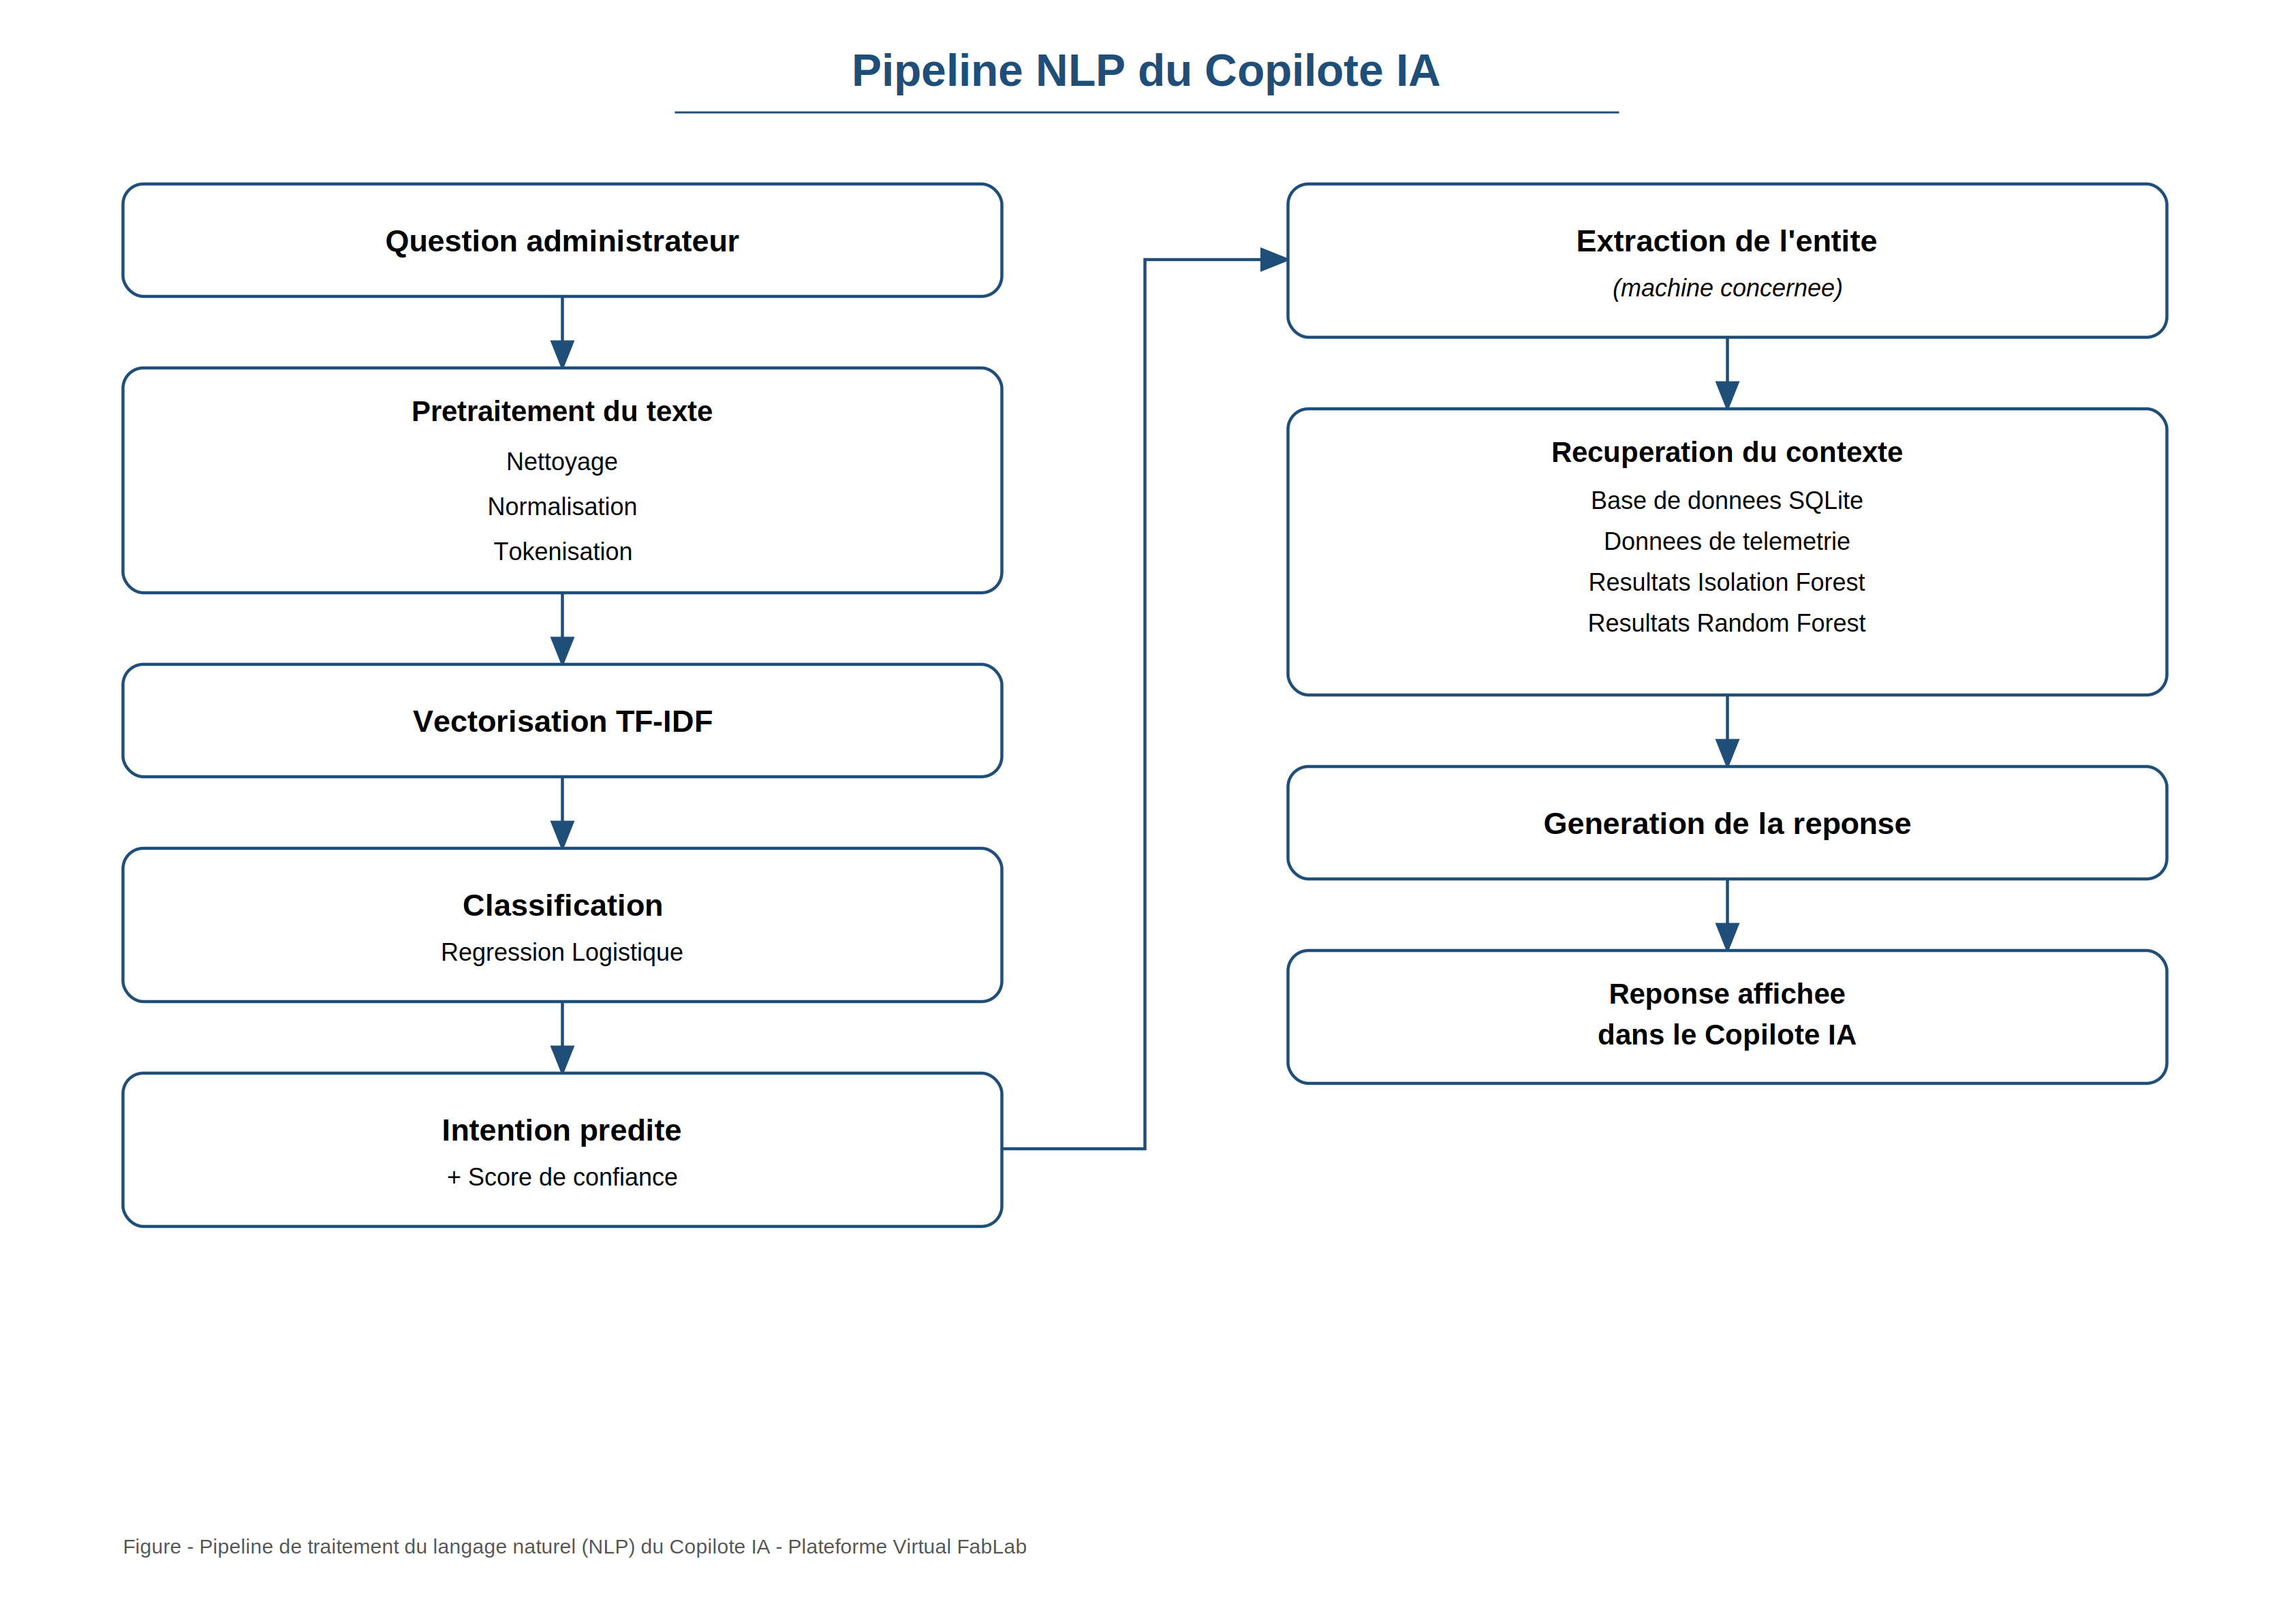
\includegraphics[width=0.95\textwidth]{images/pipeline_nlp_copilot.png}}
{\fbox{\parbox[c][5.8cm][c]{0.88\textwidth}{\centering Emplacement réservé pour le workflow NLP du Copilote\\[2mm]\texttt{images/pipeline\_nlp\_copilot.png}\\[2mm]\small Administrator question $\rightarrow$ text preprocessing $\rightarrow$ TF-IDF $\rightarrow$ Logistic Regression $\rightarrow$ predicted intent and confidence $\rightarrow$ entity extraction $\rightarrow$ telemetry context retrieval $\rightarrow$ ML results $\rightarrow$ grounded response $\rightarrow$ admin interface}}}
\caption{Workflow NLP du Copilote IA de maintenance}
\label{fig:pipeline-nlp-copilot}
\end{figure}

\section{Copilote IA de maintenance}

Le Copilote IA de maintenance est un copilote d'aide à la décision combinant détection d'anomalies, prédiction du risque, classification supervisée des intentions et génération déterministe de réponses fondées sur les données. Il répond à des questions administrateur sur l'état global du FabLab, l'état d'une machine, les anomalies récentes, la machine la plus risquée, les recommandations de maintenance, les réservations et la comparaison de machines.

Le service commence par construire un contexte à partir de la base de données : liste des machines, synthèse de flotte, évaluations de maintenance, historique de télémétrie et résumé des réservations. L'extraction d'entités repère les machines par leur nom, leurs variantes avec tirets ou espaces, ainsi que les références de type \texttt{machine 1} ou \texttt{\#1}. La réponse retournée contient l'intention, la sévérité, la confiance, les machines extraites, des points de données et des recommandations.

Les réponses ne sont pas générées par un modèle de langage. Elles sont construites par des fonctions déterministes et par des textes localisés, à partir des faits observés, des scores calculés et des recommandations par règles. Cette distinction est importante : le copilote ne produit pas un diagnostic industriel autonome, mais une synthèse structurée d'aide à la décision.

\begin{table}[H]
\centering
\small
\caption{Capacités supportées par le Copilote IA de maintenance}
\label{tab:capacites-copilote-ia}
\begin{tabular}{|p{0.30\textwidth}|p{0.58\textwidth}|}
\hline
\rowcolor{SectionColor!12}
\textbf{Capacité} & \textbf{Objectif analytique} \\
\hline
Synthèse du FabLab & Résumer l'état global de la flotte, le nombre de machines avec télémétrie, les niveaux d'anomalie et les réservations en attente. \\
\hline
État d'une machine & Restituer les faits observés pour une machine donnée : statut, mesures récentes, score de santé et niveau de risque. \\
\hline
Explication du score de santé & Identifier les principaux facteurs contribuant au risque, notamment température, vibration, durée d'utilisation, erreurs et tendance récente. \\
\hline
Anomalies récentes & Lister les machines présentant un statut d'avertissement ou critique, afin de prioriser la surveillance. \\
\hline
Risque le plus élevé & Repérer la machine dont le score de risque de maintenance est le plus important dans la flotte. \\
\hline
Recommandation de maintenance & Fournir une action indicative fondée sur les anomalies, les facteurs de risque et les règles de recommandation. \\
\hline
Comparaison de machines & Comparer deux machines à partir de leurs scores de santé et de risque, sans établir de diagnostic industriel. \\
\hline
Synthèse des réservations & Présenter le nombre de réservations totales, en attente, approuvées, rejetées et prévues le jour même. \\
\hline
\end{tabular}
\end{table}

\section{Intégration dans la plateforme}

L'intégration backend est exposée par le routeur FastAPI \texttt{/admin/ai}. Les endpoints vérifiés sont notamment :

\begin{itemize}
    \item \texttt{/admin/ai/monitoring/overview} ;
    \item \texttt{/admin/ai/monitoring/machines/\{machine\_id\}} ;
    \item \texttt{/admin/ai/copilot/query} et \texttt{/admin/ai/copilot} ;
    \item \texttt{/admin/ai/model-status}, \texttt{/admin/ai/predict-sample} et \texttt{/admin/ai/train}.
\end{itemize}

Le routeur applique la dépendance \texttt{require\_admin}, ce qui réserve l'accès aux utilisateurs administrateurs.

Côté frontend, le composant \texttt{AiCopilotWidget} vérifie que l'utilisateur connecté possède le rôle \texttt{admin}. Il affiche un bouton flottant et un panneau de conversation, puis envoie les questions vers \texttt{/admin/ai/copilot/query}. L'historique de conversation est conservé localement dans l'état React du composant et n'est pas persisté dans la base de données.

\begin{figure}[H]
\centering
\IfFileExists{images/screenshot_copilot_interface.png}
{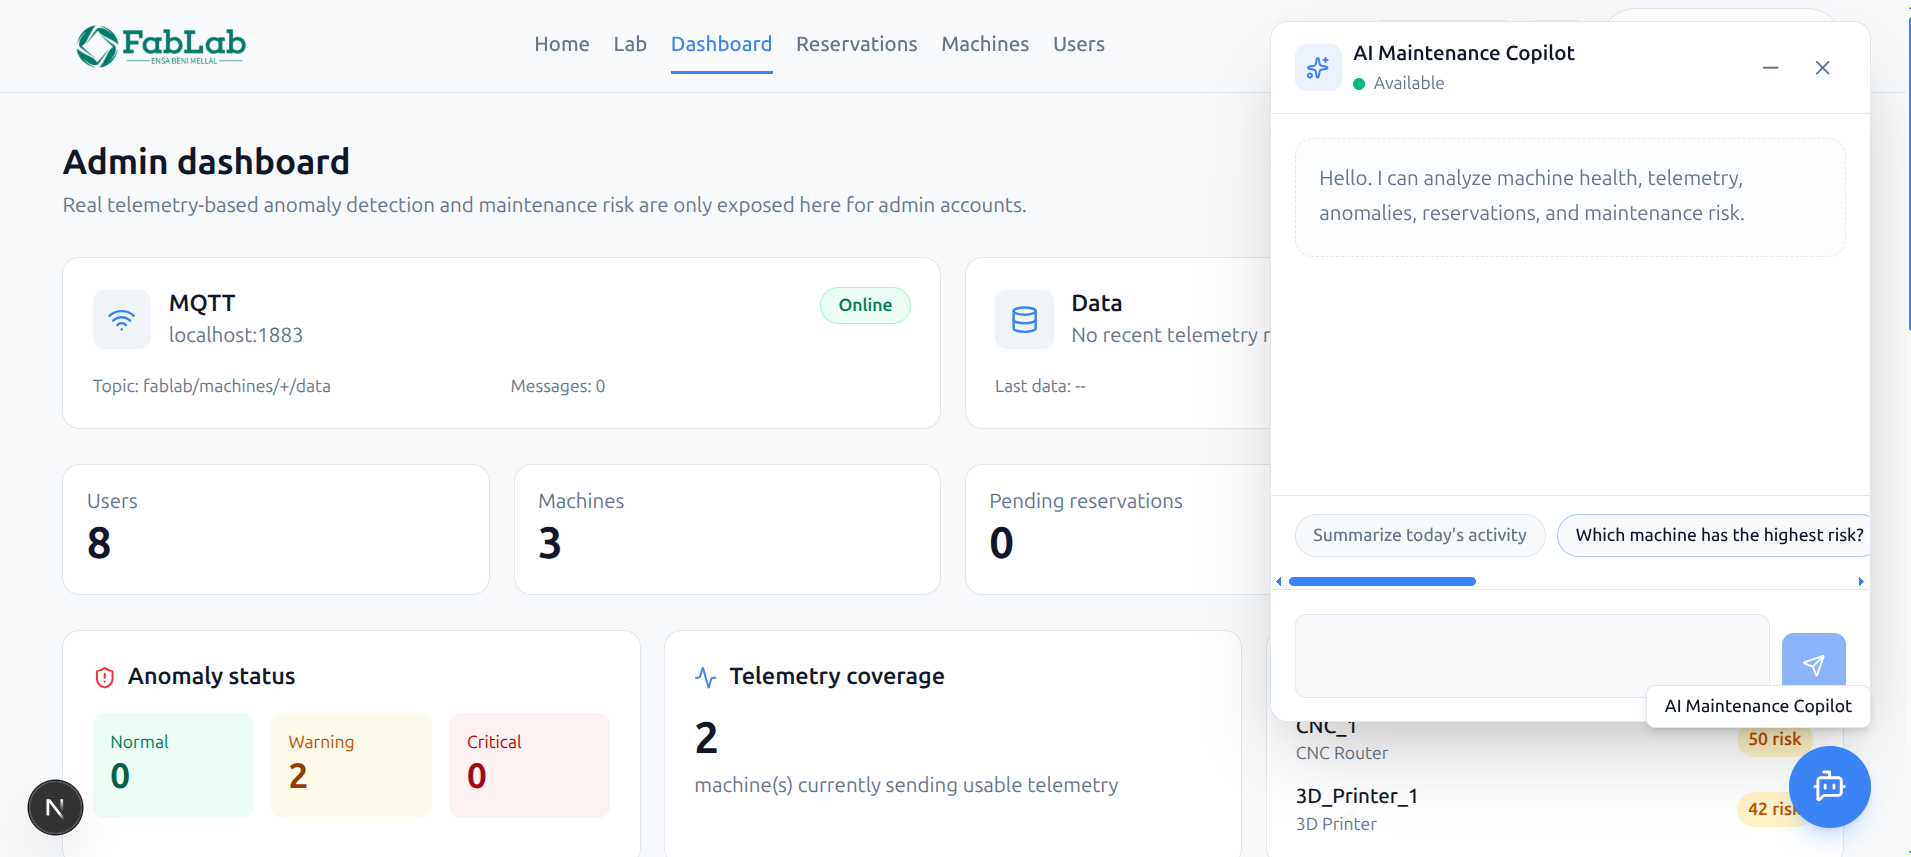
\includegraphics[width=0.82\textwidth]{images/screenshot_copilot_interface.png}}
{\fbox{\parbox[c][5cm][c]{0.82\textwidth}{\centering Emplacement réservé pour l'interface flottante du Copilote IA\\\texttt{images/screenshot\_copilot\_interface.png}}}}
\caption{Interface flottante du Copilote IA de maintenance}
\label{fig:screenshot-copilot-interface}
\end{figure}

\section{Évaluation et validation}

Les métriques disponibles concernent le classifieur NLP d'intentions. Le fichier de rapport du classifieur indique un jeu enrichi de 400 questions étiquetées, équilibrées sur 10 intentions avec 40 exemples par intention. Ce jeu est séparé en 280 exemples d'entraînement, 60 exemples de validation et 60 exemples de test.

\begin{table}[H]
\centering
\small
\caption{Métriques disponibles pour la classification NLP des intentions}
\label{tab:metrics-nlp-intents}
\begin{tabular}{|p{0.32\textwidth}|p{0.25\textwidth}|p{0.25\textwidth}|}
\hline
\rowcolor{SectionColor!12}
\textbf{Métrique} & \textbf{Validation} & \textbf{Test} \\
\hline
Accuracy & 0,6833 & 0,8333 \\
\hline
Précision macro & 0,7278 & 0,8452 \\
\hline
Rappel macro & 0,6833 & 0,8333 \\
\hline
F1-score macro & 0,6793 & 0,8355 \\
\hline
Taille de l'échantillon & 60 & 60 \\
\hline
\end{tabular}
\end{table}

Ces résultats doivent être interprétés avec prudence, car le jeu de test reste limité et provient du même corpus annoté. Ils montrent toutefois que l'enrichissement des formulations améliore nettement la classification tout en conservant le même pipeline TF-IDF et Logistic Regression.

L'évaluation actuelle du module Data Science et IA porte principalement sur le comportement en inférence, la cohérence des sorties produites, l'intégration dans la plateforme et les métriques disponibles pour le classifieur NLP. Cette validation permet de vérifier le fonctionnement global du prototype et la bonne exploitation des données simulées. Une validation quantitative plus large, appuyée sur des jeux de test indépendants et sur des données réelles, constitue toutefois une étape complémentaire nécessaire pour apprécier plus finement la robustesse des modèles dans un contexte opérationnel.

\begin{table}[H]
\centering
\small
\caption{Synthèse de l'évaluation du module Data Science et IA}
\label{tab:synthese-evaluation-ds-ia}
\begin{tabular}{|>{\raggedright\arraybackslash}p{0.30\textwidth}|>{\raggedright\arraybackslash}p{0.30\textwidth}|>{\raggedright\arraybackslash}p{0.30\textwidth}|}
\hline
\rowcolor{SectionColor!12}
\textbf{Composant} & \textbf{Validation réalisée} & \textbf{Validation complémentaire proposée} \\
\hline
Isolation Forest & Chargement du modèle, production du score d'anomalie, tests d'inférence et intégration dans la plateforme. & Validation sur données réelles, étude de stabilité et comparaison avec des scénarios connus. \\
\hline
Random Forest & Vérification des variables d'entrée, des classes et des prédictions produites. & Évaluation quantitative sur un jeu de test indépendant et plus large. \\
\hline
Classifieur NLP & Accuracy, précision, rappel, F1-score et matrice de confusion sur le corpus enrichi. & Validation sur un jeu indépendant et davantage de questions réelles. \\
\hline
Copilote IA & Tests d'accès administrateur, classification d'intentions, extraction d'entités et génération de réponses fondées sur les données. & Évaluation utilisateur et analyse qualitative des réponses. \\
\hline
\end{tabular}
\end{table}

\section{Limites}

Les limites principales du module sont liées à la nature des données et au périmètre du prototype. La télémétrie est simulée, ce qui permet de tester les flux et les interfaces, mais ne remplace pas une collecte issue de capteurs installés sur des machines réelles. Les modèles entraînés ne sont donc pas validés industriellement.

Le jeu de données NLP a été enrichi et équilibré, ce qui améliore les métriques disponibles. Il reste toutefois limité au périmètre des intentions supportées par le backend et doit être consolidé par des questions réelles collectées en usage. Le système fonctionne comme un classifieur d'intentions supervisé, pas comme un agent conversationnel génératif. Les réponses sont déterministes et fondées sur les données disponibles.

Enfin, les recommandations doivent être comprises comme une aide à la décision. Elles distinguent les faits observés, les scores inférés et les actions conseillées, sans prétendre diagnostiquer avec certitude une panne mécanique ou électrique.

\section{Conclusion du chapitre}

Ce chapitre a isolé la contribution Data Science et IA du projet Virtual FabLab. Le module combine l'ingestion de données MQTT simulées, l'extraction de caractéristiques, la détection d'anomalies par Isolation Forest, l'estimation du risque par Random Forest, la classification supervisée des intentions par TF-IDF et Logistic Regression, ainsi qu'un Copilote IA de maintenance réservé aux administrateurs.

L'ensemble constitue une couche d'aide à la décision adaptée à un prototype académique. Les résultats doivent cependant rester contextualisés : les données sont simulées, les métriques Machine Learning industrielles sont absentes pour les modèles de maintenance, et une validation future sur données réelles reste nécessaire.

\chapter{Validation et résultats}

\section{Introduction}

Ce chapitre présente la validation fonctionnelle de la plateforme \textbf{Virtual FabLab}, les résultats obtenus, ainsi que les limites actuelles du travail réalisé. Après la description de l'implémentation dans le chapitre précédent, il s'agit ici de vérifier que les principales fonctionnalités répondent aux besoins définis : consultation du laboratoire virtuel, gestion des machines, réservation, simulation 3D, authentification, administration et communication entre le frontend et le backend.

La validation effectuée reste adaptée au contexte d'un projet de fin d'études. Elle porte principalement sur le bon fonctionnement des parcours utilisateurs et administrateurs, ainsi que sur la cohérence des échanges entre les différentes couches de l'application. Les parties liées à l'IoT et à la Data Science sont abordées avec prudence, car elles reposent encore sur des données simulées ou sur une base préparée pour une intégration future avec des équipements réels.

\section{Validation fonctionnelle de la plateforme}

\subsection{Tests du frontend}

Les tests du frontend ont porté sur les interfaces développées avec Next.js. L'objectif était de vérifier que les pages principales sont accessibles, lisibles et cohérentes avec les rôles des utilisateurs. Les interfaces testées incluent notamment la page d'accueil, le laboratoire 3D, la page des machines, les réservations, le tableau de bord administrateur et les pages de gestion.

La navigation a également été vérifiée afin de s'assurer que l'utilisateur peut passer d'un module à l'autre sans rupture de parcours. Les redirections vers la page de connexion sont déclenchées lorsque l'utilisateur n'est pas authentifié, tandis que les pages réservées à l'administrateur restent protégées pour les utilisateurs étudiants.

La partie simulation 3D a été validée à travers le chargement de la scène du FabLab, la sélection des machines et la visualisation des actions associées. Les modules de simulation CNC et imprimante 3D ont été testés avec des fichiers de démonstration afin de vérifier l'affichage des trajectoires, la progression de la simulation et la gestion des fichiers non valides. Ces tests confirment le caractère opérationnel de la simulation dans un objectif pédagogique, même si elle ne reproduit pas encore l'ensemble des phénomènes physiques réels.

\subsection{Tests du backend FastAPI}

La validation du backend FastAPI a concerné l'authentification, les routes protégées, les API REST et la gestion des erreurs. Le mécanisme d'authentification repose sur un jeton JWT généré lors de la connexion. Ce jeton permet ensuite d'accéder aux routes protégées selon le rôle de l'utilisateur.

Les tests effectués ont permis de vérifier les comportements suivants :

\begin{itemize}
    \item création d'un compte utilisateur avec des données valides ;
    \item connexion et récupération du jeton JWT ;
    \item accès au profil de l'utilisateur connecté ;
    \item protection des routes nécessitant une authentification ;
    \item restriction des routes administrateur aux utilisateurs autorisés ;
    \item création, consultation et traitement des réservations ;
    \item consultation et gestion des machines selon les permissions.
\end{itemize}

La validation des requêtes a également été prise en compte. Lorsque les données envoyées sont incorrectes ou incomplètes, le backend retourne des erreurs adaptées. Les principaux cas traités concernent les erreurs d'authentification, les accès interdits, les ressources inexistantes et les conflits liés aux réservations. Cette gestion permet au frontend d'afficher des messages compréhensibles et d'éviter les comportements incohérents.

\subsection{Communication frontend/backend}

La communication entre le frontend et le backend est centralisée dans la fonction utilitaire \texttt{apiRequest}. Cette fonction joue un rôle important dans l'organisation du code, car elle évite de répéter la logique d'appel API dans chaque page ou composant.

Son rôle consiste principalement à construire l'URL du backend, ajouter les en-têtes nécessaires aux échanges JSON, intégrer le token JWT lorsqu'il est disponible, puis traiter les réponses retournées par le backend. Lorsqu'une erreur HTTP est renvoyée, la fonction récupère le message d'erreur et le transforme en information exploitable par l'interface.

\begin{figure}[H]
\centering
\IfFileExists{images/api_communication.png}
{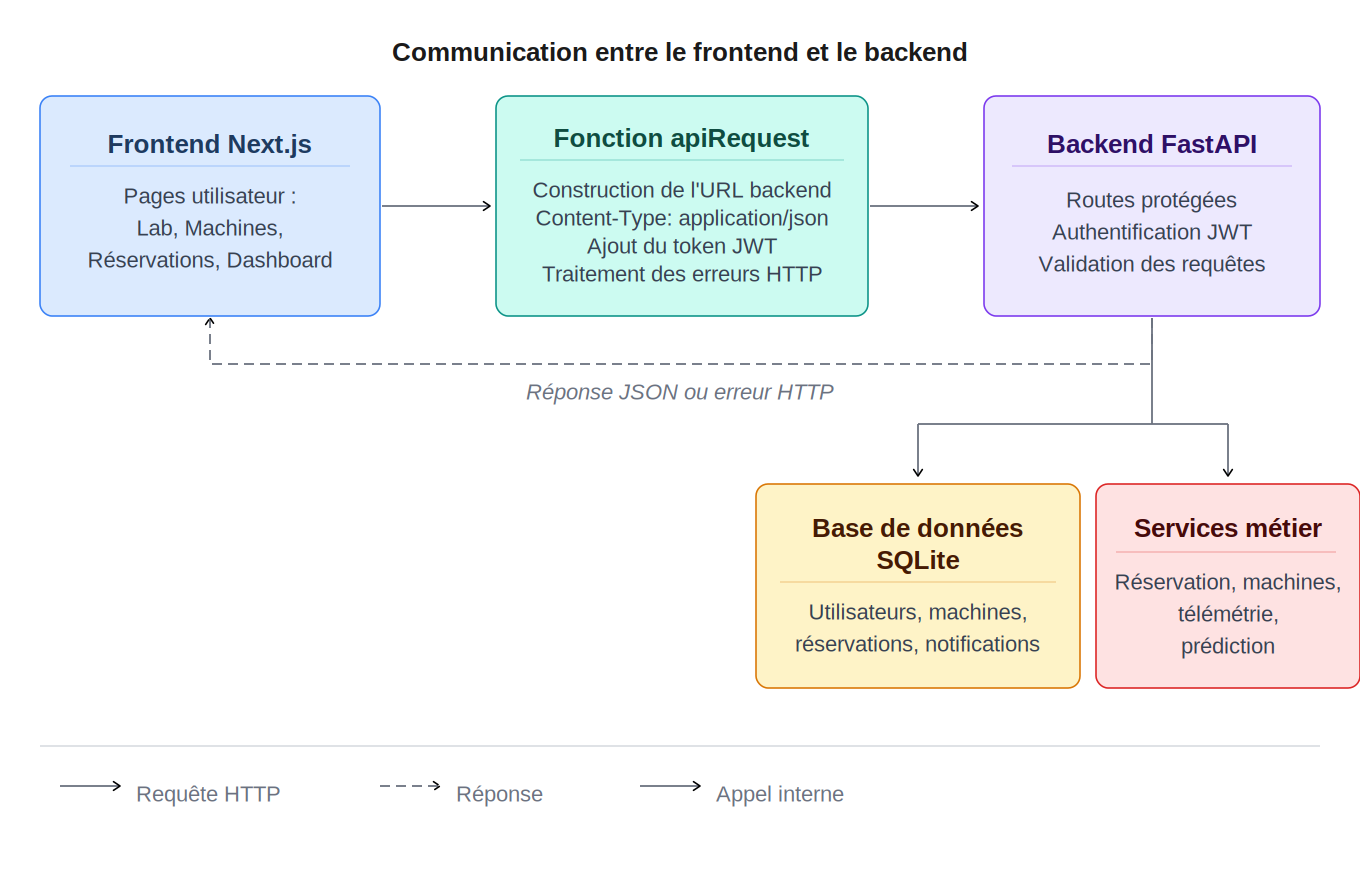
\includegraphics[width=0.9\textwidth]{images/api_communication.png}}
{\fbox{\parbox[c][5cm][c]{0.85\textwidth}{\centering Emplacement réservé pour le schéma de communication frontend/backend\\\texttt{images/api\_communication.png}}}}
\caption{Schéma de communication entre l'interface Next.js et le backend FastAPI}
\label{fig:api-communication-validation}
\end{figure}

La figure \ref{fig:api-communication-validation} illustre le principe général des échanges. Le frontend envoie une requête HTTP vers l'API FastAPI. Le backend valide la requête, applique la logique métier, interagit avec la base de données ou les services concernés, puis retourne une réponse JSON ou une erreur HTTP. Cette organisation rend la communication plus claire et facilite l'évolution de la plateforme.

\section{Résultats obtenus}

Les résultats obtenus montrent que la plateforme développée constitue un prototype fonctionnel répondant aux objectifs principaux du projet. L'application web permet à l'utilisateur de consulter les machines, accéder au laboratoire virtuel, effectuer des réservations et visualiser des simulations liées aux machines numériques.

Du côté administrateur, la plateforme permet la gestion des machines, des utilisateurs et des réservations. La séparation entre le frontend Next.js et le backend FastAPI rend l'architecture plus claire et facilite la maintenance du projet. Les routes backend assurent la persistance des données, la sécurité et l'exposition des fonctionnalités sous forme d'API REST.

La simulation 3D est opérationnelle pour représenter le FabLab virtuel et illustrer le comportement de machines telles que la CNC et l'imprimante 3D. Elle apporte une dimension visuelle et pédagogique importante au projet, en permettant à l'utilisateur d'interagir avec les machines avant une utilisation réelle.

Enfin, le projet fournit une base solide pour l'intégration future de l'IoT et de la Data Science. Les mécanismes liés à la télémétrie, à la supervision et à l'analyse de données sont préparés ou simulés, ce qui permet de démontrer l'orientation du système vers un FabLab connecté et intelligent sans prétendre à une validation industrielle complète.

\section{Limites actuelles et perspectives}

Malgré les résultats obtenus, certaines limites doivent être mentionnées. La première concerne la télémétrie, qui reste simulée. Les données utilisées permettent de tester les flux et les interfaces, mais elles ne remplacent pas des mesures réelles issues de capteurs installés sur des machines physiques.

La deuxième limite concerne l'absence de connexion directe avec de vraies machines IoT. Les scénarios de communication MQTT et de supervision sont préparés, mais ils nécessitent encore une validation avec des équipements réels. De même, la simulation 3D ne reproduit pas totalement le comportement réel des machines, notamment les contraintes mécaniques, les vibrations, les variations thermiques ou les défauts de fabrication.

Plusieurs perspectives peuvent être envisagées pour améliorer la plateforme :

\begin{itemize}
    \item intégrer un broker MQTT réel et des messages provenant de machines physiques ;
    \item ajouter des capteurs IoT pour collecter des mesures de température, vibration ou vitesse ;
    \item enrichir la maintenance prédictive à partir de données historiques réelles ;
    \item améliorer le réalisme de la simulation CNC et imprimante 3D ;
    \item développer un dashboard analytique plus avancé avec des courbes, alertes et indicateurs de performance.
\end{itemize}

Ces perspectives montrent que la solution actuelle peut servir de base évolutive. Elle permet déjà de valider l'architecture et les principaux parcours fonctionnels, tout en laissant une marge d'amélioration importante vers une plateforme plus connectée et plus intelligente.

\section{Conclusion}

Ce chapitre a présenté la validation fonctionnelle de la plateforme, les résultats obtenus ainsi que les limites actuelles du projet. Les tests réalisés confirment le fonctionnement des principaux modules : frontend, backend, authentification, gestion des machines, réservations, simulation 3D et communication API.

La plateforme Virtual FabLab répond ainsi aux objectifs essentiels du projet, tout en restant réaliste sur les limites liées à la simulation et à l'absence de machines IoT réelles. Elle constitue une base fonctionnelle et évolutive pour de futurs travaux autour de la supervision, de l'analyse de données et de la maintenance prédictive dans un FabLab connecté.


% ─── Conclusion générale ──────────────────────────────────────────
\chapterstar{Conclusion générale}

Ce projet de fin d'études avait pour objectif de concevoir et de réaliser une plateforme web de FabLab virtuel intelligent, destinée à faciliter la gestion des machines, la visualisation de l'environnement de fabrication et la supervision des équipements dans un contexte académique.

Les travaux réalisés ont permis de mettre en place une plateforme web fonctionnelle intégrant une simulation 3D du FabLab, un système de communication basé sur le protocole MQTT pour la réception des données de télémétrie, une détection d'anomalies, une évaluation du risque de maintenance, une classification supervisée d'intentions et un Copilote IA de maintenance réservé à l'administrateur. Un tableau de bord administrateur complète la solution en assurant le suivi des équipements, des réservations et des principaux indicateurs de supervision.

Dans la version actuelle, les données de télémétrie utilisées sont simulées. Cette approche a permis de valider l'architecture globale de la solution, les flux de communication MQTT, le stockage des données et le fonctionnement du module d'analyse. Les résultats obtenus ne constituent donc pas une validation industrielle, mais une base expérimentale pour une future intégration dans un environnement réel.

Les perspectives de ce projet concernent principalement la connexion de la plateforme à des capteurs et à des machines réelles, la constitution de jeux de données plus larges, le réentraînement des modèles sur de la télémétrie réelle, l'enrichissement du corpus NLP, le support multilingue, l'amélioration de l'explicabilité, l'intégration optionnelle d'un LLM strictement ancré dans les données et la validation dans un FabLab opérationnel.

% ─── Bibliographie et webographie ─────────────────────────────────
\clearpage
\renewcommand{\bibname}{Bibliographie et webographie}
\markboth{Bibliographie et webographie}{Bibliographie et webographie}
\addcontentsline{toc}{chapter}{Bibliographie et webographie}
\begin{thebibliography}{99}

\bibitem{Gershenfeld}
Gershenfeld, Neil A.,
\textit{Fab: The Coming Revolution on Your Desktop: From Personal Computers to Personal Fabrication},
Basic Books, New York, 2005, ISBN~978-0-465-02745-3.

\bibitem{Schwab}
Schwab, Klaus,
\textit{The Fourth Industrial Revolution},
World Economic Forum, Geneva, 2016, ISBN~978-1-944835-00-2.

\bibitem{Kagermann2013}
Kagermann, Henning, Wahlster, Wolfgang et Helbig, Johannes,
\textit{Recommendations for Implementing the Strategic Initiative INDUSTRIE 4.0: Securing the Future of German Manufacturing Industry},
Final report of the Industrie 4.0 Working Group, acatech -- National Academy of Science and Engineering, 2013.

\bibitem{LeeIndustry2015}
Lee, Jay, Bagheri, Behrad et Kao, Hung-An,
``A Cyber-Physical Systems Architecture for Industry 4.0-Based Manufacturing Systems'',
\textit{Manufacturing Letters}, vol.~3, 2015, p.~18--23,
\url{https://doi.org/10.1016/j.mfglet.2014.12.001}.

\bibitem{IoT}
Greengard, Samuel,
\textit{The Internet of Things},
MIT Press, Cambridge, 2015, ISBN~978-0-262-52773-6.

\bibitem{Jardine2006}
Jardine, Andrew K. S., Lin, Daming et Banjevic, Dragan,
``A Review on Machinery Diagnostics and Prognostics Implementing Condition-Based Maintenance'',
\textit{Mechanical Systems and Signal Processing}, vol.~20, no~7, 2006, p.~1483--1510,
\url{https://doi.org/10.1016/j.ymssp.2005.09.012}.

\bibitem{LeePHM2014}
Lee, Jay, Wu, Fangji, Zhao, Wenyu, Ghaffari, Masoud, Liao, Linxia et Siegel, David,
``Prognostics and Health Management Design for Rotary Machinery Systems: Reviews, Methodology and Applications'',
\textit{Mechanical Systems and Signal Processing}, vol.~42, no~1--2, 2014, p.~314--334,
\url{https://doi.org/10.1016/j.ymssp.2013.06.004}.

\bibitem{Liu2008}
Liu, Fei Tony, Ting, Kai Ming et Zhou, Zhi-Hua,
``Isolation Forest'',
\textit{Proceedings of the 8th IEEE International Conference on Data Mining}, IEEE, 2008,
\url{https://doi.org/10.1109/ICDM.2008.17}.

\bibitem{Breiman2001}
Breiman, Leo,
``Random Forests'',
\textit{Machine Learning}, vol.~45, no~1, 2001, p.~5--32,
\url{https://doi.org/10.1023/A:1010933404324}.

\bibitem{Salton1988}
Salton, Gerard et Buckley, Christopher,
``Term-Weighting Approaches in Automatic Text Retrieval'',
\textit{Information Processing \& Management}, vol.~24, no~5, 1988, p.~513--523,
\url{https://doi.org/10.1016/0306-4573(88)90021-0}.

\bibitem{Cox1958}
Cox, David R.,
``The Regression Analysis of Binary Sequences'',
\textit{Journal of the Royal Statistical Society: Series B (Methodological)}, vol.~20, no~2, 1958, p.~215--232,
\url{https://doi.org/10.1111/j.2517-6161.1958.tb00292.x}.

\bibitem{JurafskyMartin2026}
Jurafsky, Daniel et Martin, James H.,
\textit{Speech and Language Processing: An Introduction to Natural Language Processing, Computational Linguistics, and Speech Recognition with Language Models},
3e éd., manuscrit en ligne, version du 6 janvier 2026,
\url{https://web.stanford.edu/~jurafsky/slp3/}.

\bibitem{TurDeMori2011}
Tur, Gokhan et De Mori, Renato,
\textit{Spoken Language Understanding: Systems for Extracting Semantic Information from Speech},
John Wiley \& Sons, Chichester, 2011, ISBN~978-0-470-68824-3.

\bibitem{ML}
Géron, Aurélien,
\textit{Hands-On Machine Learning with Scikit-Learn, Keras, and TensorFlow: Concepts, Tools, and Techniques to Build Intelligent Systems},
2e éd., O'Reilly Media, Sebastopol, 2019, ISBN~978-1-492-03263-2.

\bibitem{Pedregosa2011}
Pedregosa, Fabian et al.,
``Scikit-learn: Machine Learning in Python'',
\textit{Journal of Machine Learning Research}, vol.~12, 2011, p.~2825--2830.

\bibitem{Few2006}
Few, Stephen,
\textit{Information Dashboard Design: The Effective Visual Communication of Data},
O'Reilly Media, Sebastopol, 2006, ISBN~978-0-596-10016-2.

\bibitem{NextjsDocs}
Vercel,
\textit{Documentation officielle de Next.js},
\url{https://nextjs.org/docs},
consultée le 18 juillet 2026.

\bibitem{ReactDocs}
Meta Open Source,
\textit{Documentation officielle de React},
\url{https://react.dev/},
consultée le 18 juillet 2026.

\bibitem{FastAPIDocs}
FastAPI,
\textit{Documentation officielle de FastAPI},
\url{https://fastapi.tiangolo.com/},
consultée le 18 juillet 2026.

\bibitem{ThreejsDocs}
Three.js,
\textit{Documentation officielle de Three.js},
\url{https://threejs.org/docs/},
consultée le 18 juillet 2026.

\bibitem{ReactThreeFiberDocs}
pmndrs,
\textit{Documentation officielle de React Three Fiber},
\url{https://r3f.docs.pmnd.rs/},
consultée le 18 juillet 2026.

\bibitem{MQTTDocs}
OASIS,
\textit{MQTT Version 5.0, OASIS Standard},
\url{https://docs.oasis-open.org/mqtt/mqtt/v5.0/os/mqtt-v5.0-os.html},
consultée le 18 juillet 2026.

\bibitem{SQLiteDocs}
SQLite,
\textit{Documentation officielle de SQLite},
\url{https://www.sqlite.org/docs.html},
consultée le 18 juillet 2026.

\bibitem{JWTIntro}
Jones, Michael B., Bradley, John et Sakimura, Nat,
\textit{JSON Web Token (JWT), RFC 7519},
Internet Engineering Task Force, 2015,
\url{https://www.rfc-editor.org/rfc/rfc7519}.

\bibitem{ScikitLearnDocs}
Scikit-learn,
\textit{User Guide},
\url{https://scikit-learn.org/stable/user_guide.html},
consultée le 18 juillet 2026.

\bibitem{TailwindDocs}
Tailwind Labs,
\textit{Documentation officielle de Tailwind CSS},
\url{https://tailwindcss.com/docs},
consultée le 18 juillet 2026.

\bibitem{BlenderDocs}
Blender Foundation,
\textit{Documentation officielle de Blender},
\url{https://docs.blender.org/},
consultée le 18 juillet 2026.

\end{thebibliography}

\end{document}
